%
% Based on the template for Doctoral 
% Theses at Uppsala University. 
% The template is based on    
% the layout and typography used for      
% dissertations in the Acta Universitatis 
% Upsaliensis series                      
% Ver 5.2 - 2012-08-08                  
% Latest version available at:            
%   http://ub.uu.se/thesistemplate            
%                                         
%%%%%%%%%%%%%%%%%%%%%%%%%%%%%%%%%%%%%%%%%%%


\documentclass{UUThesisTemplate}

% Package to determine wether XeTeX is used
\usepackage{ifxetex}

\ifxetex
	% XeTeX specific packages and settings
	% Language, diacritics and hyphenation
	\usepackage[babelshorthands]{polyglossia}
	\setmainlanguage{english}
	\setotherlanguages{swedish}

	% Font settings
	\setmainfont{Times New Roman}
	\setromanfont{Times New Roman}
	\setsansfont{Arial}
	\setmonofont{Courier New}
\else
	% Plain LaTeX specific packages and settings
	% Language, diacritics and hyphenation
    % Use English and Swedish languages. 
	\usepackage[swedish,english]{babel} 

	% Font settings
	\usepackage{type1cm}
	\usepackage[latin1]{inputenc}
	\usepackage[T1]{fontenc}
	\usepackage{mathptmx}
	
	% Enable scaling of images on import
	\usepackage{graphicx}
    \graphicspath{{./Images/}}
    \usepackage{hyperref}

    \usepackage[usenames,dvipsnames]{xcolor}
    
\fi


% Tables
\usepackage{booktabs}
\usepackage{tabularx}

% Document links and bookmarks
\usepackage{url}
\usepackage{hyperref} 
\hypersetup{
  pdftitle={Detection and Quantification of Small Changes in MRI Volumes},    % title
  pdfauthor={Mariana Bustamante},     % author
  urlcolor=blue,   % color of external links
  citecolor=OliveGreen, % color of links to bibliography
}
\usepackage{breakurl}

% Numbering of headings down to the subsection level
\numberingdepth{subsection}

% Including headings down to the sub(sub)section level in contents
\contentsdepth{subsubsection}


\title{Detection and Quantification of Small Changes in MRI Volumes}
\subtitle{Centre for Image Analysis}
\author{Mariana Bustamante}
\titlepagelogo{UU_logo_sv_42.eps}
\providecommand{\makehalftitle}{%
	\begin{center}%
		\ifx\@publisher\relax\ifx\@series\relax Half Title Dummy Page\par \fi\fi%
		\MakeUppercase{\@publisher}\par%
		\@series\par%
		\@serialnumber\par%
	\end{center}%
}



\abstractdummy{
	\begin{abstract}
		Please use no more than 300 words and avoid mathematics or complex script.
	\end{abstract}
}


\begin{document}
\frontmatter
    % Creates the front matter (title page(s), abstract, list of papers)
    % for either a Comprehensive Summary or a Monograph.
    % Authors of Comprehensive Summaries use this front matter 
    \frontmatterCS 
    % Monograph authors use this front matter 
    %\frontmatterMonograph 
 
   % Optional dedication
   \dedication{Dedicated to all hard-working \\doctoral students at Uppsala University}
 
    % Environment used to create a list of papers
    %\begin{listofpapers}
    %	\item A Paper Discussed in this Thesis \label{apaperlabel}
    %\end{listofpapers}
    
    
    \begingroup
        % To adjust the indentation in your table of contents, uncomment and enter the widest numbers for each level
        %  E.g.  \settocnumwidth{widest chapter number}{widest section number}{widest subsection number}...{...}
       %  \settocnumwidth{5}{4}{5}{3}{3}{3}
        \tableofcontents
    \endgroup
    
    % Optional tables
    %\listoftables
    %\listoffigures

\mainmatter
     \chapter{Introduction}

\section{Description of the problem}
When a person suffers an accident that produces trauma to the head, one of the first things that should be performed is an MRI of the brain region in order to spot possible brain injuries. If the damage is large, a medical specialist can usually recognize which parts of the brain have been affected without automated help. However, if the damage is minor, it is generally much harder for the doctor to figure out what could be the consequences of the injury. \\

For this particular project we have the following conditions: A patient's brain is scanned, producing a first MRI just after receiving trauma to the head. The patient has not received extensive damage, and so the MRI comes out as expected from a medical specialist. After a period of three to twelve months later, a new MRI of the same patient is taken and is compared with the initial MRI.

It is assumed that if there are symptoms produced as a consequence of the accident, then there must be differences in the brain of the patient, even when the differences might be too small to see with the naked eye.\\


The goal of this project is to analyse and test different registration and morphometry methods, in order to compare this type of brain MRIs and produce information on the differences between them. 

The final result of the project should be a tool that allows the medical specialist to do the comparison on his or her own.


\section{Importance}

Manual examination of MRI studies suffers from many problems. The study can be affected specially by acquisition related factors such as:
\begin{itemize}
\item One cannot assume a one-to-one correspondence between slices from one acquisition to the next in order to make side-by-side comparisons.
\item A different scanner may be used in every examination, producing a scan which will have different signal characteristics.
\item Often, scanning parameters are not the same form one acquisition to the next.
\item Change can present itself in many ways. The radiologist is required to assimilate all this data before making a decision, which often is quite difficult.
\end{itemize}

A very important part of change detention is therefore not simply the detection of change but the separation of acquisition-related change from disease-related change. Also, methods that produce objective, reproducible and accurate metrics of disease course are of great interest since the change in appearance over time is essential to understanding disease course \cite{review1}.

Also, it is not enough to be able to determine if there are differences, since from a clinical standpoint, knowing where and how changes have occurred is as important as knowing that they have occurred \cite{review1}.\\


From a practical point of view, it is also very important for the patients to be able to obtain a correct diagnosis, specially if the symptoms they are suffering are hard to explain or subjective, as it is common with non-extensive brain injuries.

\section{Related Works}
Many related works focus on inter-subject studies, which means that they compare images acquired from different individuals in order to diagnose diseases or identify abnormalities. This generally implies that the first step in the analysis process is one of \textit{spatial normalization} or \textit{inter-subject registration}, in which the aim is to reduce the anatomical variability in the volumetric brain scans.

The works of \cite{zeffiro,svensen} use this technique combined with voxelwise group analysis of functional magnetic resonance imaging (fMRI), and the works of \cite{ardekani1,jones} also use spatial normalization combined with diffusion tensor imaging in order to study brain white matter.\\

More similar works, related to the quantification of small changes in volume observed over time can be observed in \cite{holden,rey}. The results of these works are used to diagnose and evaluate disease progression and treatment.


Some other works that also use the specific techniques described later in this project are:
\begin{itemize}
\item Hajnal et al. in \cite{hajnal} and Lemieux et al. in \cite{lemieux} utilize subtraction after applying rigid registration on the volumes.
\item Rey et al. in \cite{rey} introduce the Jacobian operator of the deformation field resulting from the registration as a measure of local volume variation.
\end{itemize}


\section{Comparison of other methods}

     \chapter{Methods}

\section{Registration}
``Image registration is the process of overlaying two or more images
of the same scene taken at different times, from different viewpoints,
and/or by different sensors. It geometrically align two images --the
reference and sensed images.''\cite{zitova}

``Image registration is a crucial step in all image analysis tasks in
which the final information is gained from the combination of various
data sources like in image fusion, change detection, and multichannel
image restoration.''\cite{zitova}\\


The following images show a checkerboard comparison of two volumes
taken of the same patient at different times. Figure \ref{before_reg}
shows the image comparison before performing affine
registration. Figure \ref{after_reg} shows the comparison of images
after the registration has been done.

\begin{figure}[htb]
  \centering
  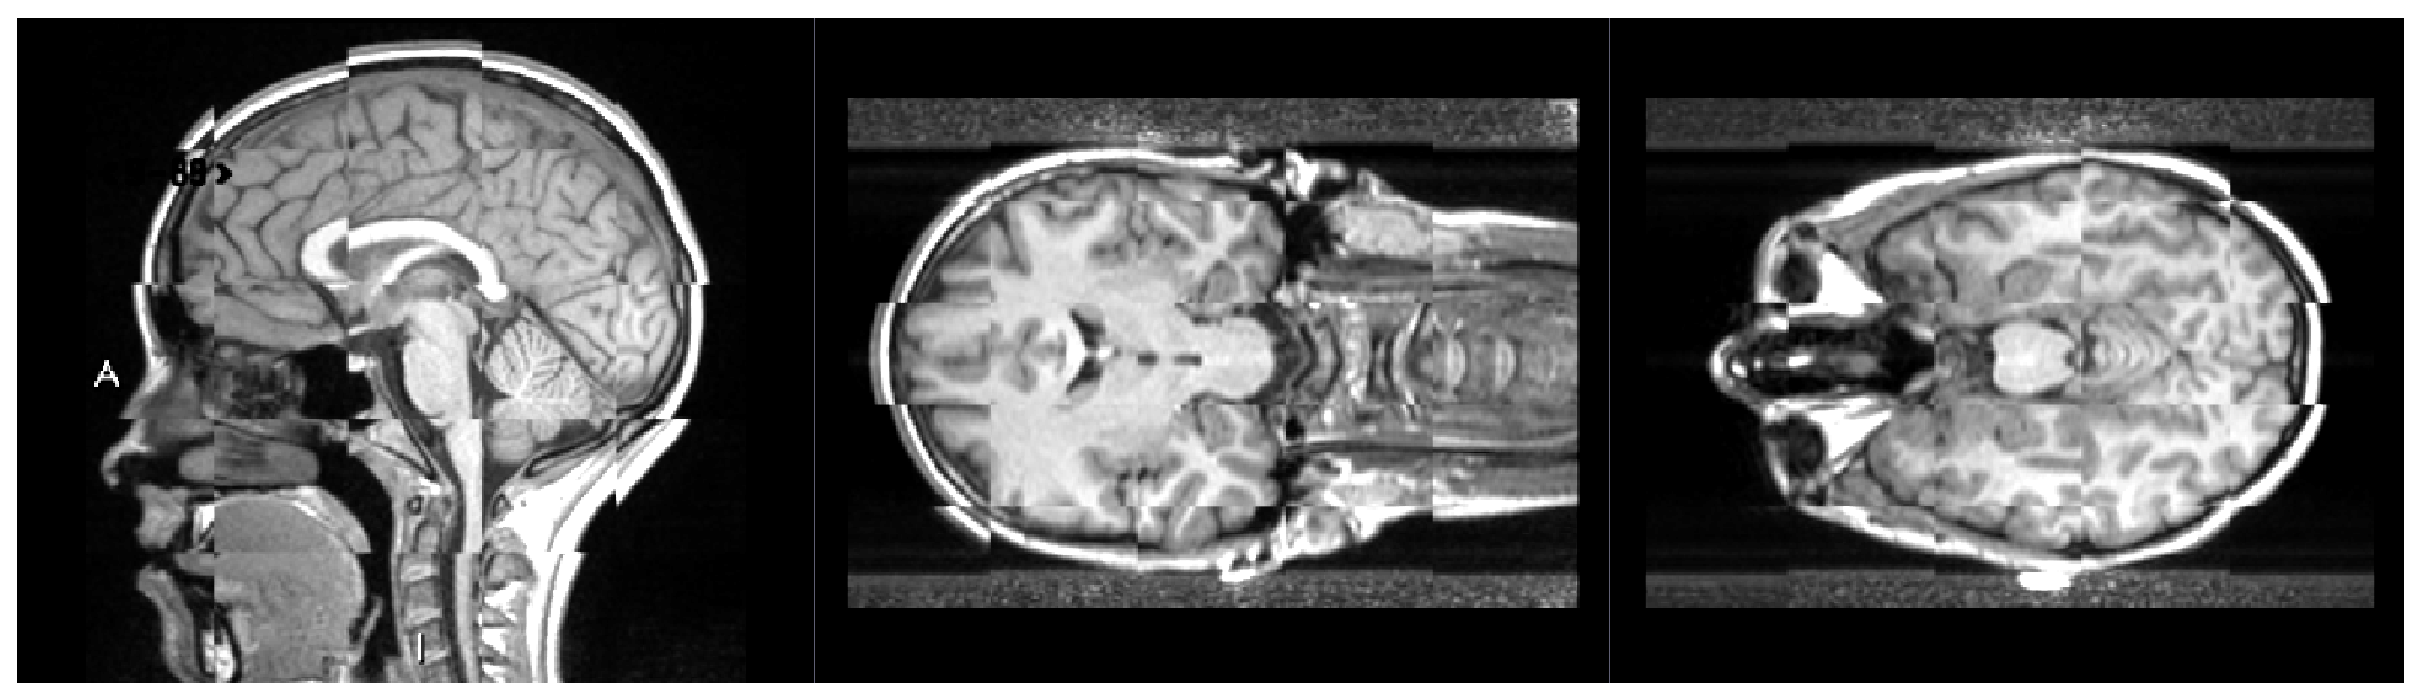
\includegraphics[scale=0.3]{before_registration.eps}
  \caption{Comparison of volumes before registration}
  \label{before_reg}
\end{figure}


\begin{figure}[htb]
  \centering
  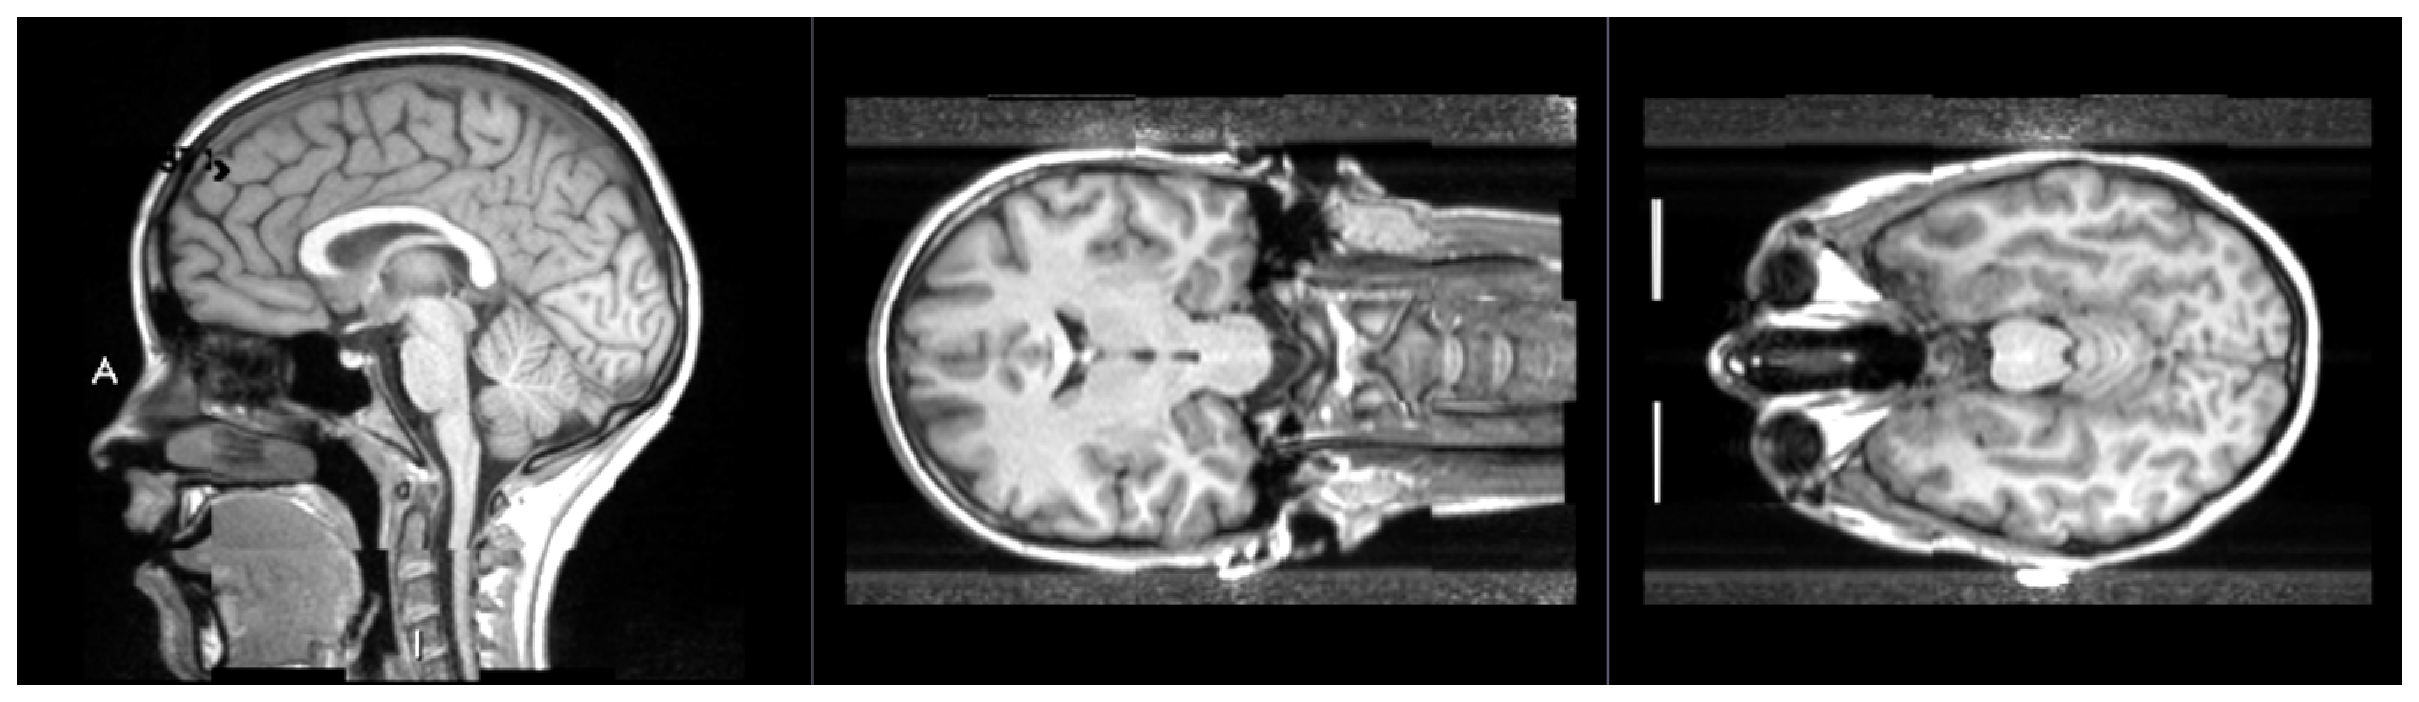
\includegraphics[scale=0.3]{after_registration.eps}
  \caption{Comparison of volumes after registration}
  \label{after_reg}
\end{figure}

The second volume has been modified using affine registration so that
the comparison between both volumes becomes much easier.\\

According to \cite{zitova}, the majority of the registration methods consist of the following steps:
\begin{enumerate}
\item \textit{Feature detection:} Salient and distinctive objects are detected.
\item \textit{Feature matching:} The correspondence between the features detected in the sensed image and those detected in the reference image is established.
\item \textit{Transform model estimation:} The type and parameters of the mapping functions are estimated. These functions align the sensed image with the reference image.
\item \textit{Image resampling and transformation:} The sensed image is transformed by means of the mapping functions.
\end{enumerate}


\subsection{Registration Methods used}
\label{sec:reg_methods}
There are many different methods to accomplish registration between
images or volumes. In this project only a few of these methods were
used based on experiments performed with some of the available
methods. The chosen procedures were the ones that behaved better
under the specific conditions of this work.


\subsubsection{Affine Registration}
In geometry, an \textit{affine transformation} or an \textit{affinity}
is a transformation which preserves straight lines (i.e., all points
lying on a line initially still lie on a line after the
transformation) and ratios of distances between points lying on a
straight line. It does not necessarily preserve angles or lengths, but
does have the property that sets of parallel lines will remain
parallel to each other after an affine transformation \cite{affine_t}. \\

The implementation of affine registration used during this project is
the one included in \textit{3D Slicer} version 4.1. 

The application is able to register two images together using an
affine transform and mutual information, and it allows the user to
modify quite a few parameters
in order to obtain the expected result.\\

If you would like to know more about this implementation of affine
registration please refer to the module webpage:

\url{http://wiki.slicer.org/slicerWiki/index.php/Documentation/4.1/Modules/AffineRegistration}

\subsubsection{B-Spline Registration}
In the mathematical subfield of numerical analysis, a
\textit{B-spline} is a spline function that has minimal support with
respect to a given degree, smoothness, and domain partition.

However, in computer graphics, the term \textit{B-spline} frequently
refers to a spline curve parametrized by spline functions that are
expressed as linear combinations of \textit{B-splines} (in the
mathematical sense explained above) \cite{bspline}.\\

Just like in the case of affine registration, the implementation of
B-Spline registration used during this project is the one included in
\textit{3D Slicer} version 4.1. 

The application divides the volumes into a grid of user-defined size
in which each line is a B-spline that will be modified by the
registration to create a transform that aligns the two volumes.\\

If you would like to know more about this implementation of B-spline
registration please refer to the module webpage:

\url{http://wiki.slicer.org/slicerWiki/index.php/Documentation/4.1/Modules/BSplineDeformableRegistration}


\subsubsection{BRAINS Demon Warp Registration}
As with the registration methods explained before, \textit{BRAINS
  Demon Warp} registration is implemented as a module in \textit{3D
  Slicer} version
4.1.\\

The module works by using the ITK filter based on Thirion's Demons
algorithm, in which the main idea is to consider the objects
boundaries in one image as semi-permeable membranes and to let the
other image, considered as a deformable grid model, diffuse through
these interfaces, by the action of effectors situated within the
membranes. \cite{thirion}.

An important characteristic of this implementation, that was
particularly useful for this project, is that it can produce a
\textit{deformation field} as the output of the registration. A
deformation field is a vector image in which each point is a vector
that indicates the amount of deformation necessary
at that point in order to align the volumes.\\


If you would like to know more about the implementation of
\textit{BRAINS Demon Warp} registration please refer to the module
webpage:

\url{http://wiki.slicer.org/slicerWiki/index.php/Documentation/4.1/Modules/BRAINSDemonWarp}


\section{Morphometry}
Morphometry refers to the measurement of external form. More
specifically, \textit{brain morphometry} is concerned with the
measurement of brain structures and changes thereof during
development, aging, learning, disease and evolution. Its goal is to
derive specific information from noninvasive neuroimaging data of live
brains, typically obtained from magnetic resonance imaging (MRI); and
to quantify the anatomical features of the brain in terms of shape,
mass and volume \cite{brmorph}.\\

In general, brain morphometry can be divided into three different methods: \textit{deformation-based}, \textit{tensor-based} and \textit{voxel-based} morphometry. Defined briefly as:
\begin{itemize}
\item \textit{Deformation-based:} Uses deformation fields to identify differences in the relative positions of structures.
\item \textit{Tensor-based:} Uses deformation fields to identify differences in the local shape of brain structures.
\item \textit{Voxel-based:} Uses voxel-wise comparison of the local concentration of grey matter.
\end{itemize}


\subsection{Morphometry methods used}
\label{sec:morph_methods}
Only \textit{tensor-based} and \textit{voxel-based} morphometry
methods where used during this project, since their outputs were
easier to adapt to our requirements.


\subsubsection{Voxel-based Morphometry}
A useful measure of structural difference among populations is derived
from a comparison of the local composition of different brain tissue
types (e.g., grey matter, white matter, etc). Voxel-based morphometry
(VBM) has been designed to be sensitive to these differences, while
discounting positional and other large scale volumetric differences in
gross anatomy.

Since its inception, VBM has become an established tool in morphometry
being used to detect cortical atrophy and differences in slender white
matter tracts \cite{ashburner}.\\

An objection to VBM is that it is sensitive to systematic shape
differences attributable to misregistration. Many potential
differences can arise as a result of movement or different positioning
of the subject in the scanner, and also there can be systematic
differences in the relative intensity of grey matter voxels compared
to white matter \cite{ashburner}.

All these differences can be detected by VBM since they are all real
differences among the data, even when they may not imply an increase
or reduction in grey matter density.\\

When VBM is used to compare MRI data of many different subjects, as is
the case many times, the process involves spatially normalizing all
the images to the same stereotactic space, extracting the gray matter
from the normalized images, smoothing, and finally performing a
statistical analysis to localize, and make inferences about, group
differences. The output from the method is a statistical parametric
map showing regions where gray matter concentration differs
significantly between groups \cite{ashburner2}.\\


For a detailed step-by-step description of VBM, please refer to
\cite{ashburner2}.

\subsubsection{Tensor-based Morphometry}
The goal of tensor-based morphometry (TBM) is to determine regional
shape differences. 

A deformation field that maps one image to another can be considered a
discrete vector field. By taking the gradients at each element of the
field, a \textit{Jacobian matrix} field is obtained, in which each element is a
tensor describing the relative positions of the neighboring
elements. Morphometric measures derived from this tensor field can be
used to locate regions with different shapes. The field obtained by
taking the determinants at each point gives a map of the structure
volumes relative to those of a reference image \cite{ashburner2}.\\

In principle, the \textit{Jacobian matrices} of the deformations (a
2nd order tensor field relating to the spatial derivatives of the
transformation) should be more reliable indicators of brain shape than
absolute deformations. Absolute deformations represent positions of
brain structures, rather than local shape, and need to be quantified
relative to some arbitrary reference position \cite{ashburner}.\\

A \textit{Jacobian matrix} contains information about the local
stretching, shearing and rotation involved in the deformation, and is
defined at each point by:

\[
J = \begin{bmatrix}
  \frac{\partial y_1}{\partial x_1} & \frac{\partial y_1}{\partial x_2} & \frac{\partial y_1}{\partial x_3} \\[0.3em]
  \frac{\partial y_2}{\partial x_1} & \frac{\partial y_2}{\partial x_2} & \frac{\partial y_2}{\partial x_3} \\[0.3em]
  \frac{\partial y_3}{\partial x_1} & \frac{\partial y_3}{\partial x_2} & \frac{\partial y_3}{\partial x_3}
\end{bmatrix}
\]\\

The form of TBM that was used in this project involves comparing
relative volumes of different brain structures, where the volumes are
derived from \textit{Jacobian determinants} at each point. According
to \cite{ashburner}, this type of morphometry is useful for studies
that have specific questions about whether growth or volume loss has
occurred, and so is appropriate for our problem.\\

The \textit{Jacobian determinant} is the determinant of the
\textit{Jacobian matrix} and is sometimes simply called ``the
Jacobian''.

For a differentiable function $f$ (a function whose derivative exists
at each point in its domain), the \textit{Jacobian determinant} of
$f$'s \textit{Jacobian matrix} at a given point gives important
information about the behavior of $f$ near that point.

For instance, if the \textit{Jacobian determinant} at a point $p$ is
positive, then $f$ preserves orientation near $p$; if it is negative,
$f$ reverses orientation. The absolute value of the \textit{Jacobian
  determinant} at $p$ gives us the factor by which the function $f$
expands or shrinks volumes near $p$ \cite{jacobian}.





     \chapter{Proposed Solutions}

\section{Tools used}
\subsection{3DSlicer}
\subsection{ITK}
\subsection{Other Tools}

\section{Voxel-based method}

\section{Tensor-based method}
     \chapter{Experiments}
This section shows the results of the experiments done with the
implemented solutions. 

The methods were tried with volumes to which artificial differences of
distinct sizes and shapes were added; and also with real patient's
volumes obtained from the Uppsala University Hospital.


\section{Experiments Conditions}

\subsection{Artificial Differences}
For this experiments, the MRIs used belong to a healthy patient and
the time difference between each exam is very short, so it is expected
of them to have no changes.

The methods were used on three distinct sizes of difference: large,
medium and small. The considered sizes are based on the comparisons
done with real patients and the sizes of the differences presented on
those cases.


\subsection{Real Differences}
For this experiment, the MRIs from three real patients with known
differences were compared using both methods.

Two of them are patients of the study for which this project was
started, and so they have very small differences that are hard to
detect with the naked eye.

The third patient has larger known differences produced by a medical
condition and its subsequent surgery.


\section{Artificial Differences Results}
The initial baseline volume without modifications used for all of the
artificial tests can be seen in the following image:

\begin{figure}[H]
  \centering
  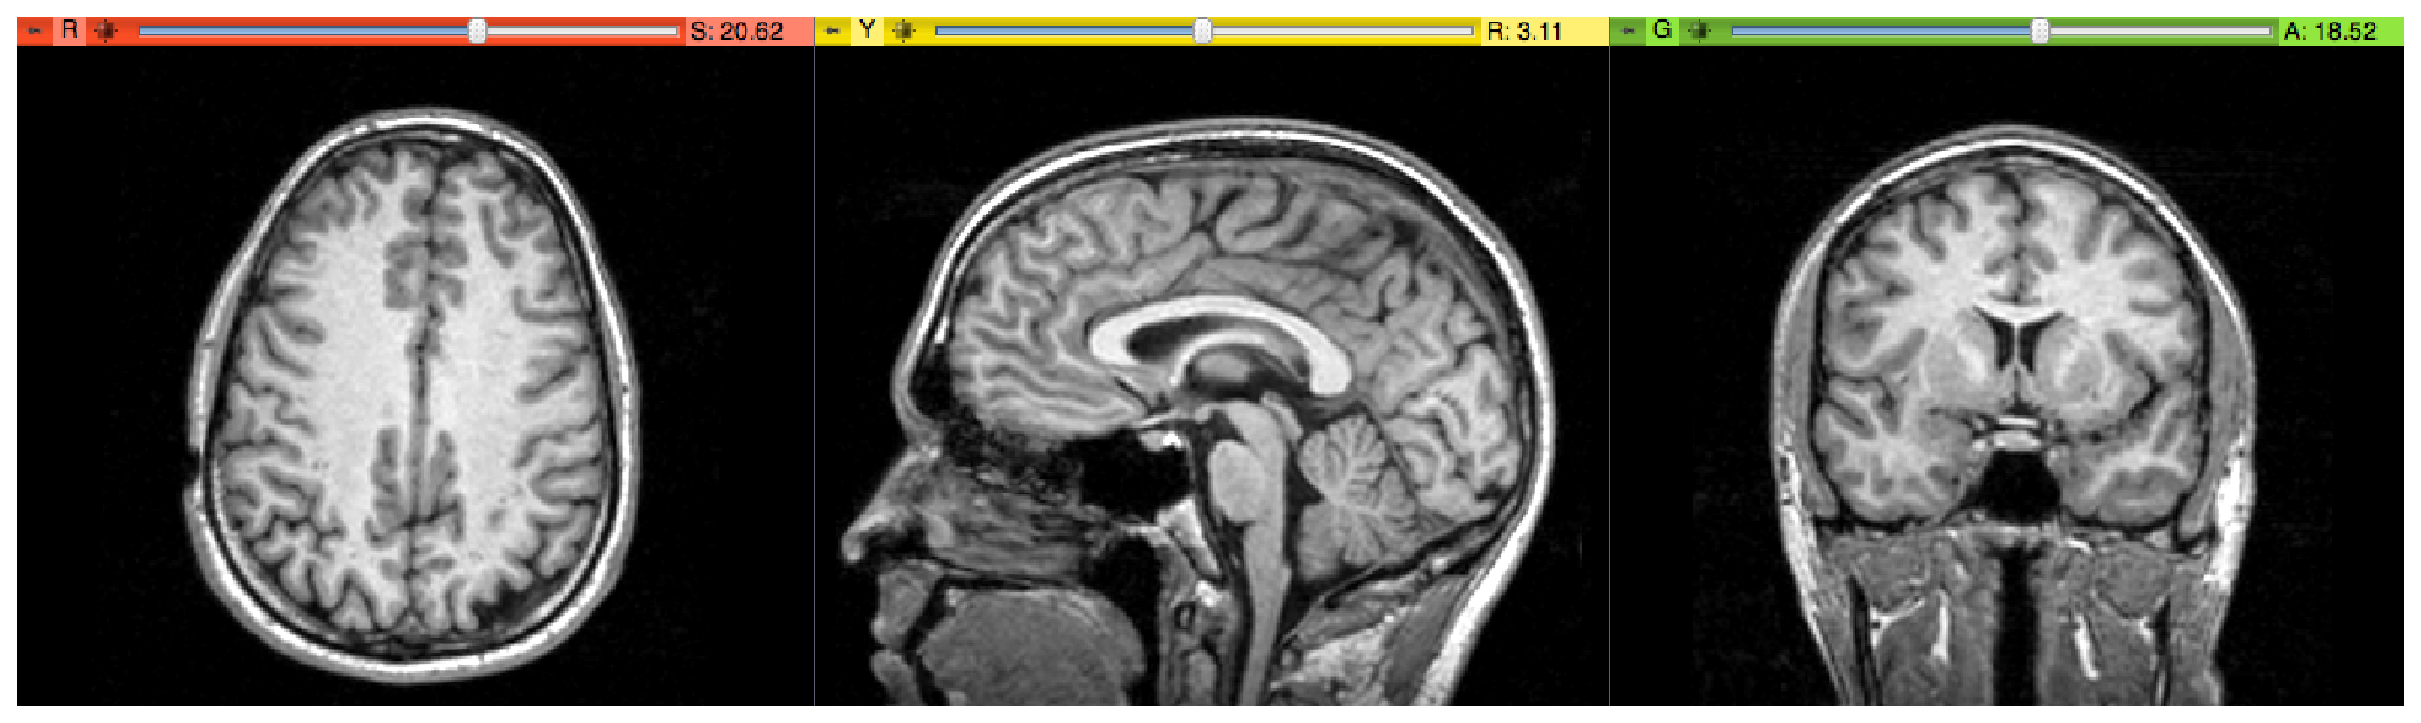
\includegraphics[scale=0.3]{/experiment_bigger/biggerA.eps}
  \caption{Artificial Differences: Baseline volume}
  \label{artificial_base}
\end{figure}

\subsection{Size: Large}
Cubes of large size where deleted from the follow-up volume to
represent areas of volume loss. The following volume was obtained:

\begin{figure}[H]
  \centering
  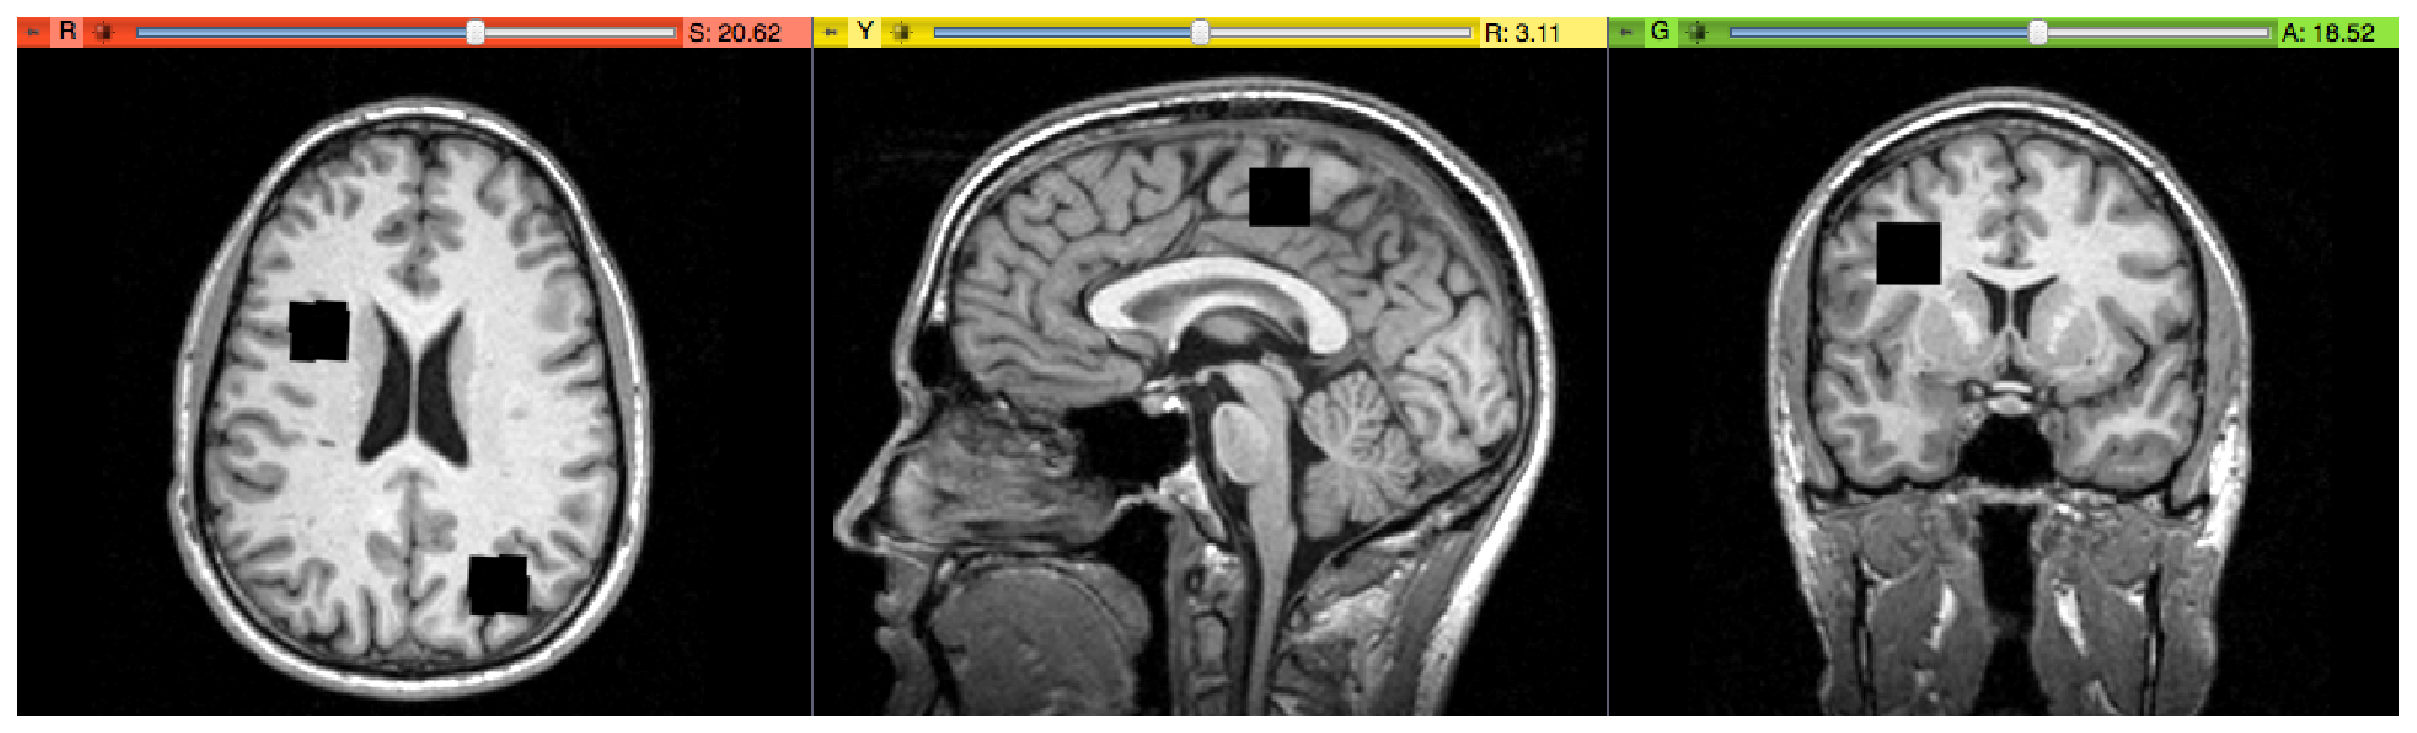
\includegraphics[scale=0.3]{/experiment_bigger/biggerB_subtracted.eps}
  \caption{Large Differences: Modified Follow-up volume}
  \label{largeB}
\end{figure}

\subsubsection{Voxel-based Method}
The result obtained with this method and large differences is pretty
good. All the differences are found and easy to see in the result.

\begin{figure}[H]
  \centering
  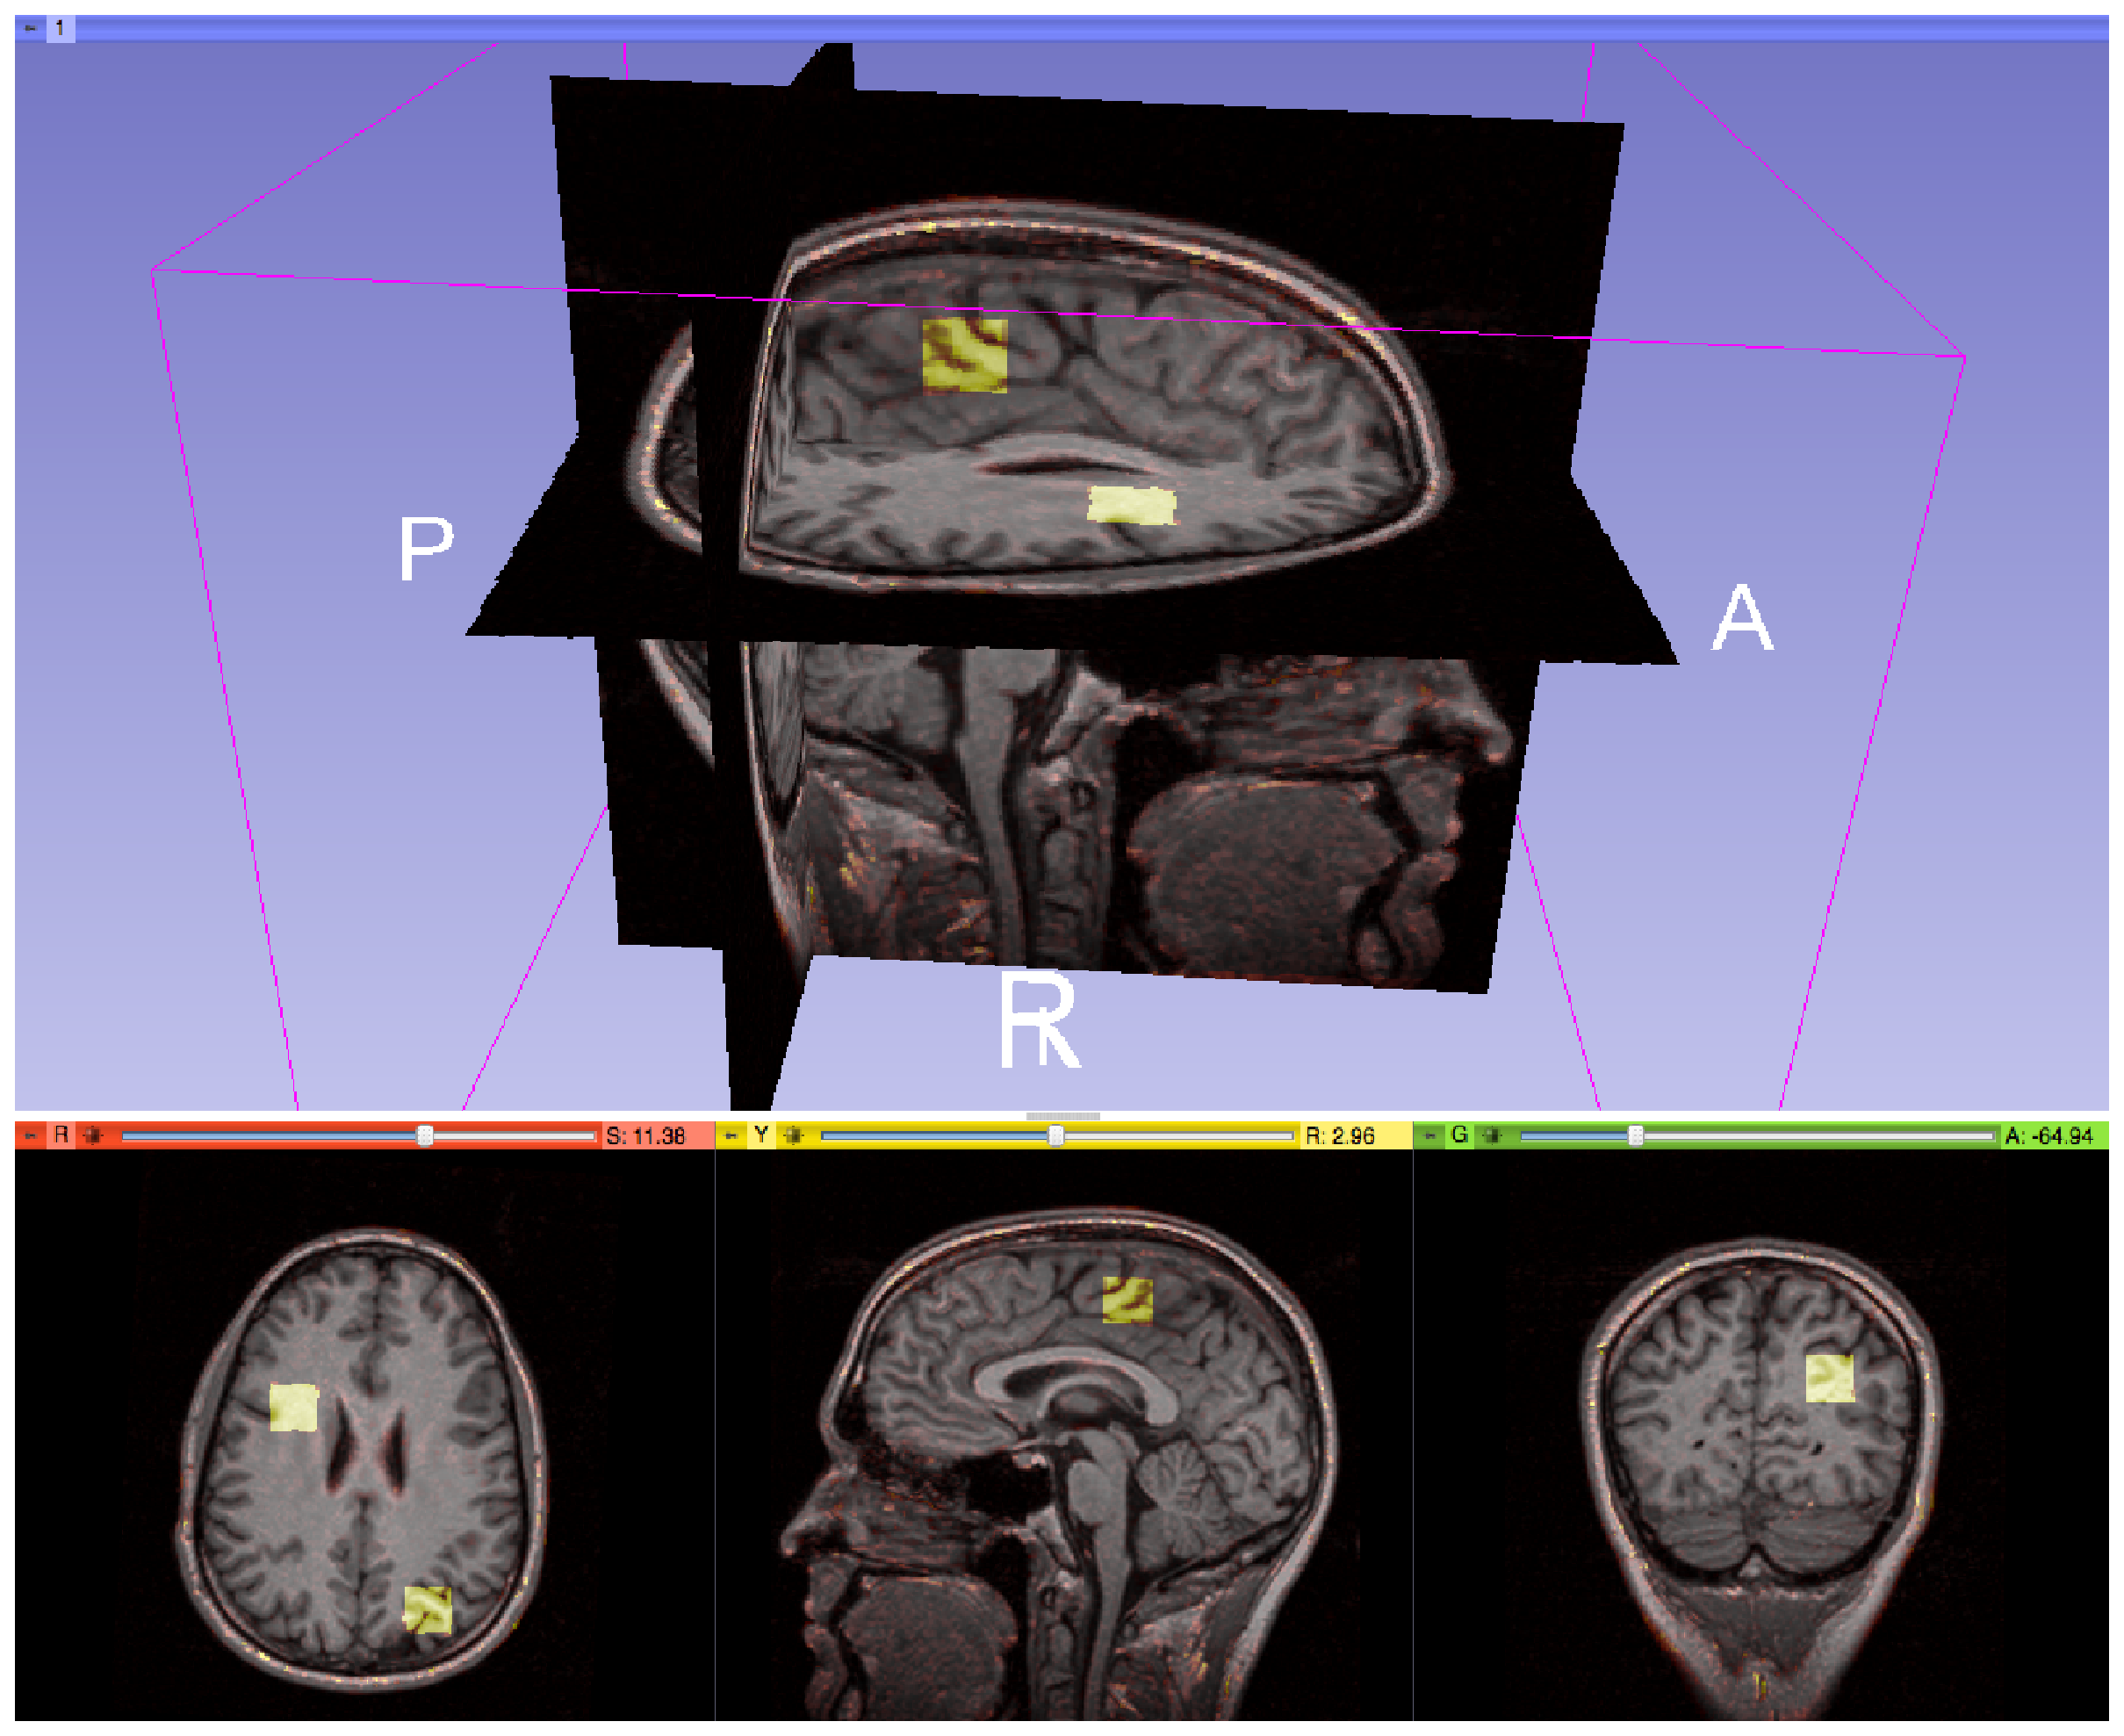
\includegraphics[scale=0.2]{/experiment_bigger/voxel_bigger1.eps}
  \caption{Artificial Large: Voxel-base method}
  \label{voxel_large1}
\end{figure}

Another angle of the result:

\begin{figure}[H]
  \centering
  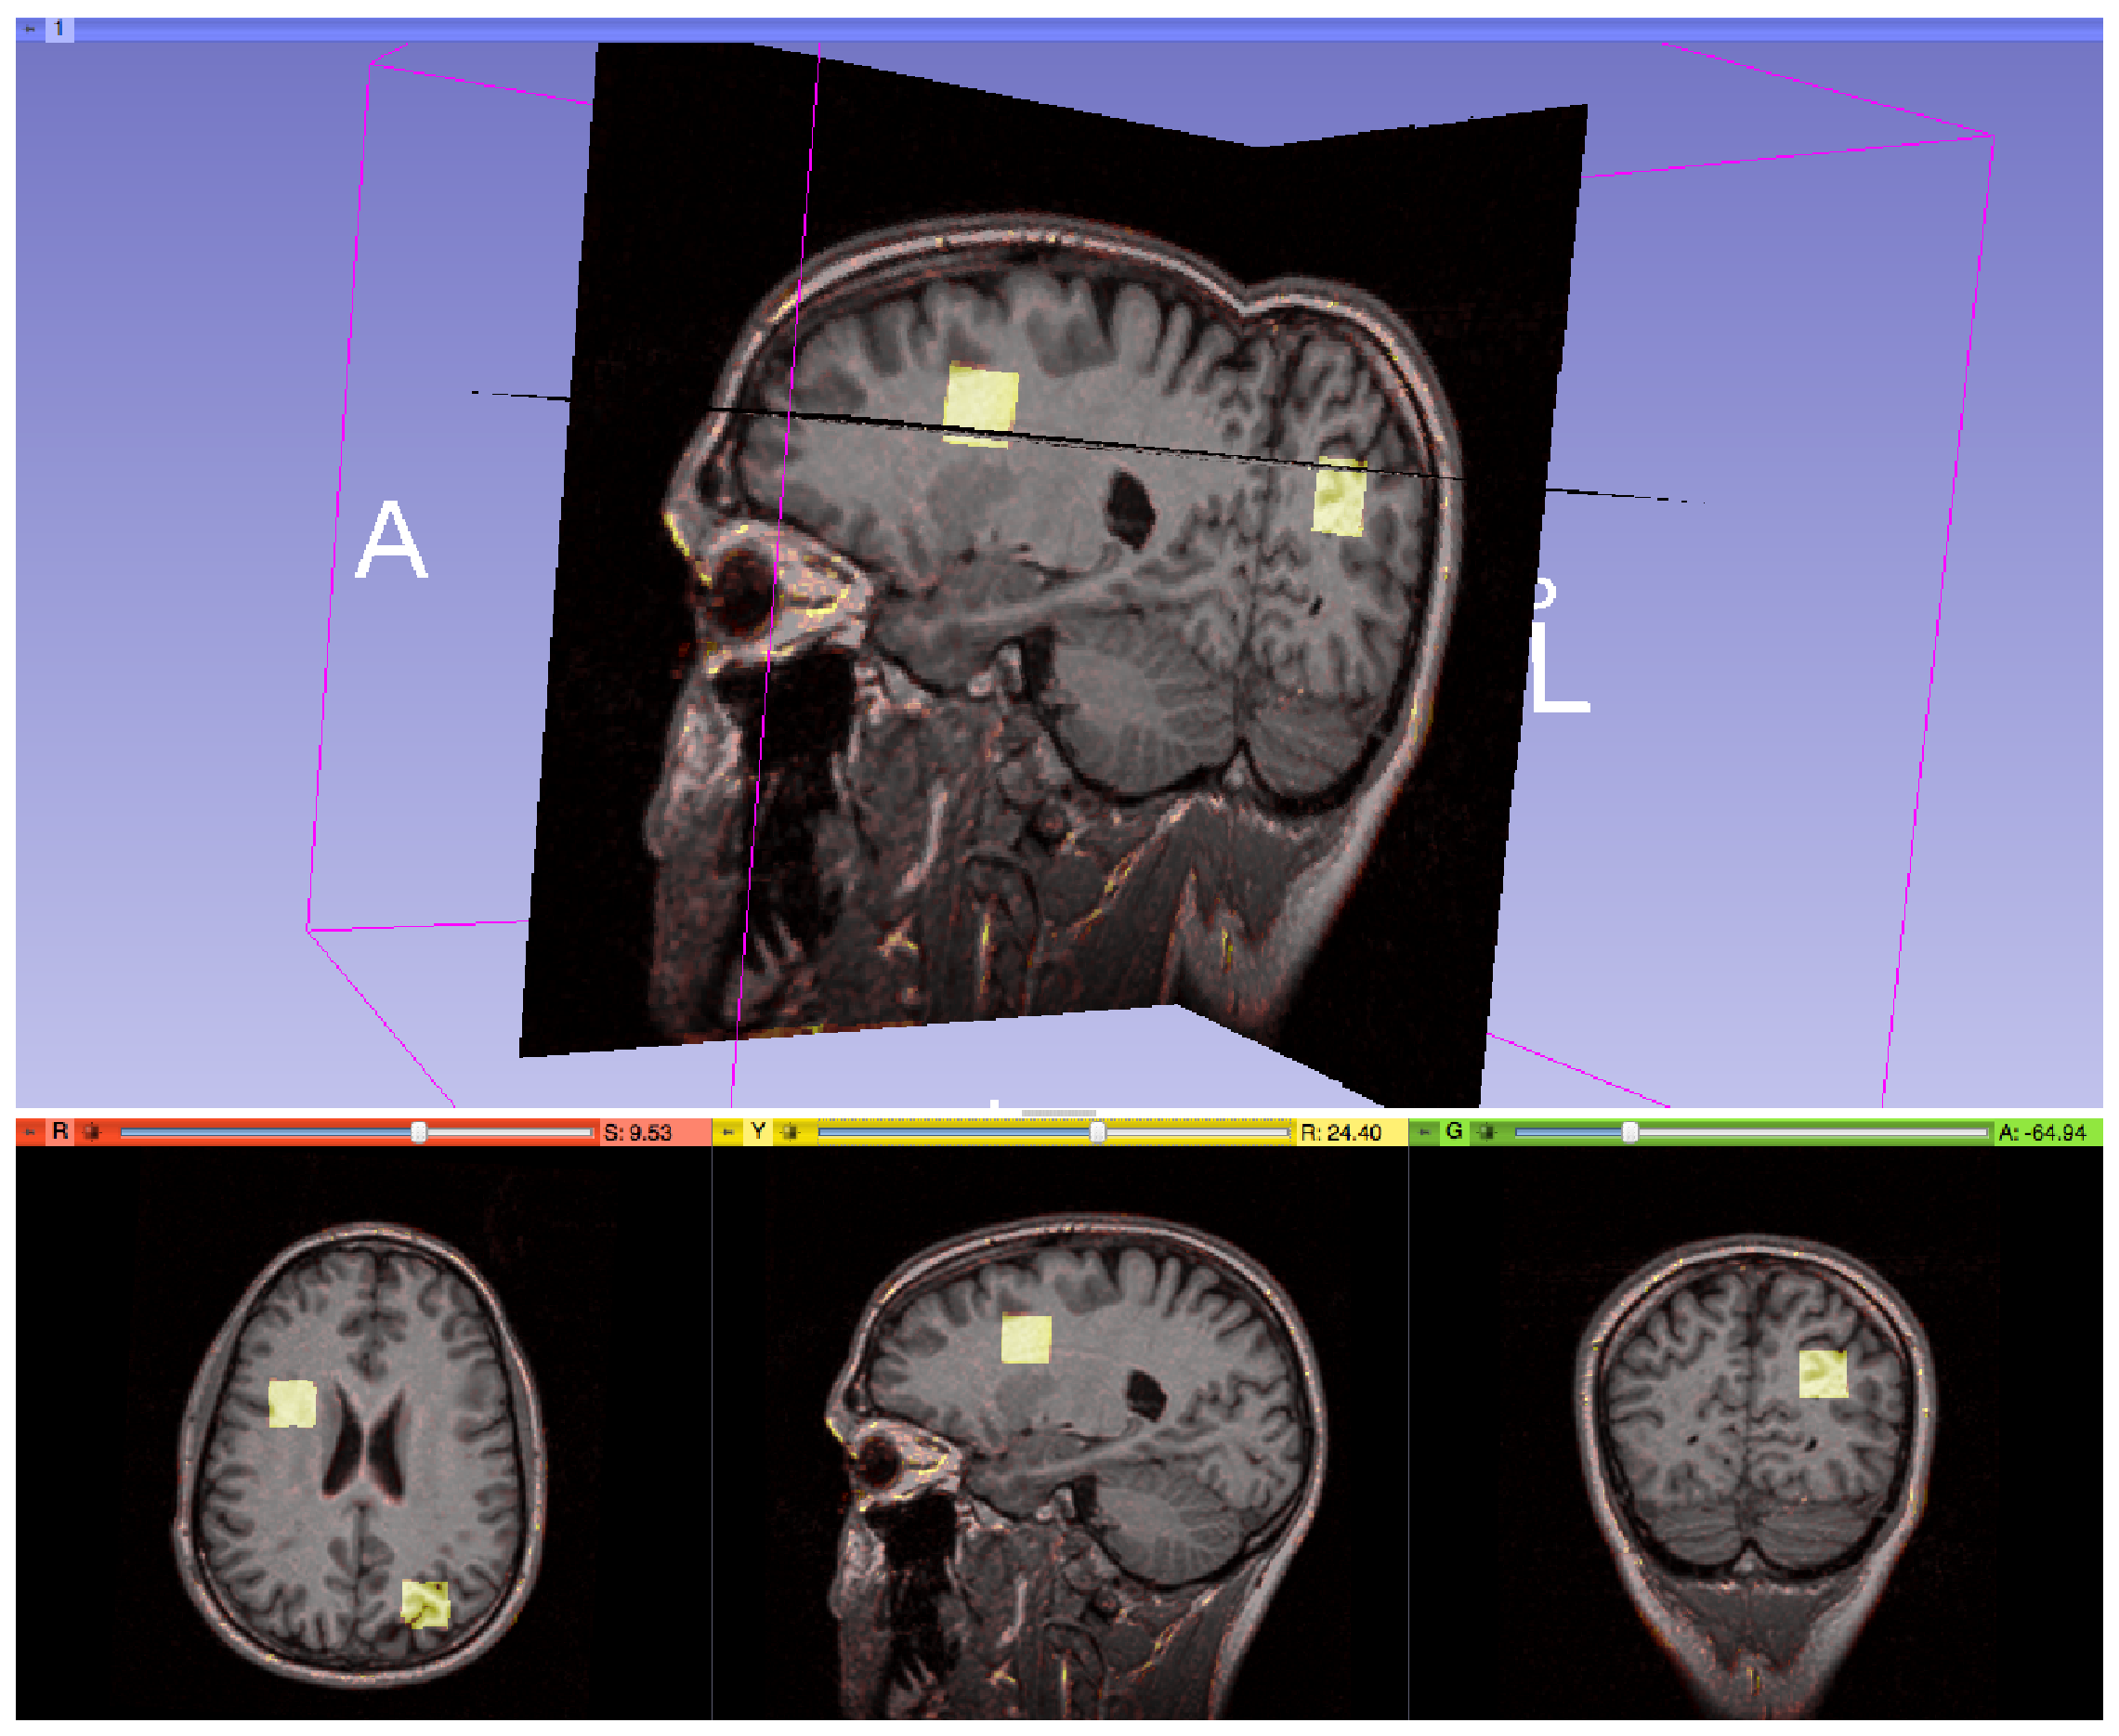
\includegraphics[scale=0.2]{/experiment_bigger/voxel_bigger2.eps}
  \caption{Artificial Large: Voxel-base method}
  \label{voxel_large2}
\end{figure}

\subsubsection{Tensor-based Method}
In the result obtained with this method the differences are easy to
find, but their borders are not properly defined. The method gives the
position of the differences but not their exact shape.

The parameters used to obtain this result are:
\begin{description}
\item \textit{Deformation field smoothing sigma:} 2.5
\item \textit{Shrinkage percentage:} 80
\item \textit{Growth percentage:} 65
\end{description}

\begin{figure}[H]
  \centering
  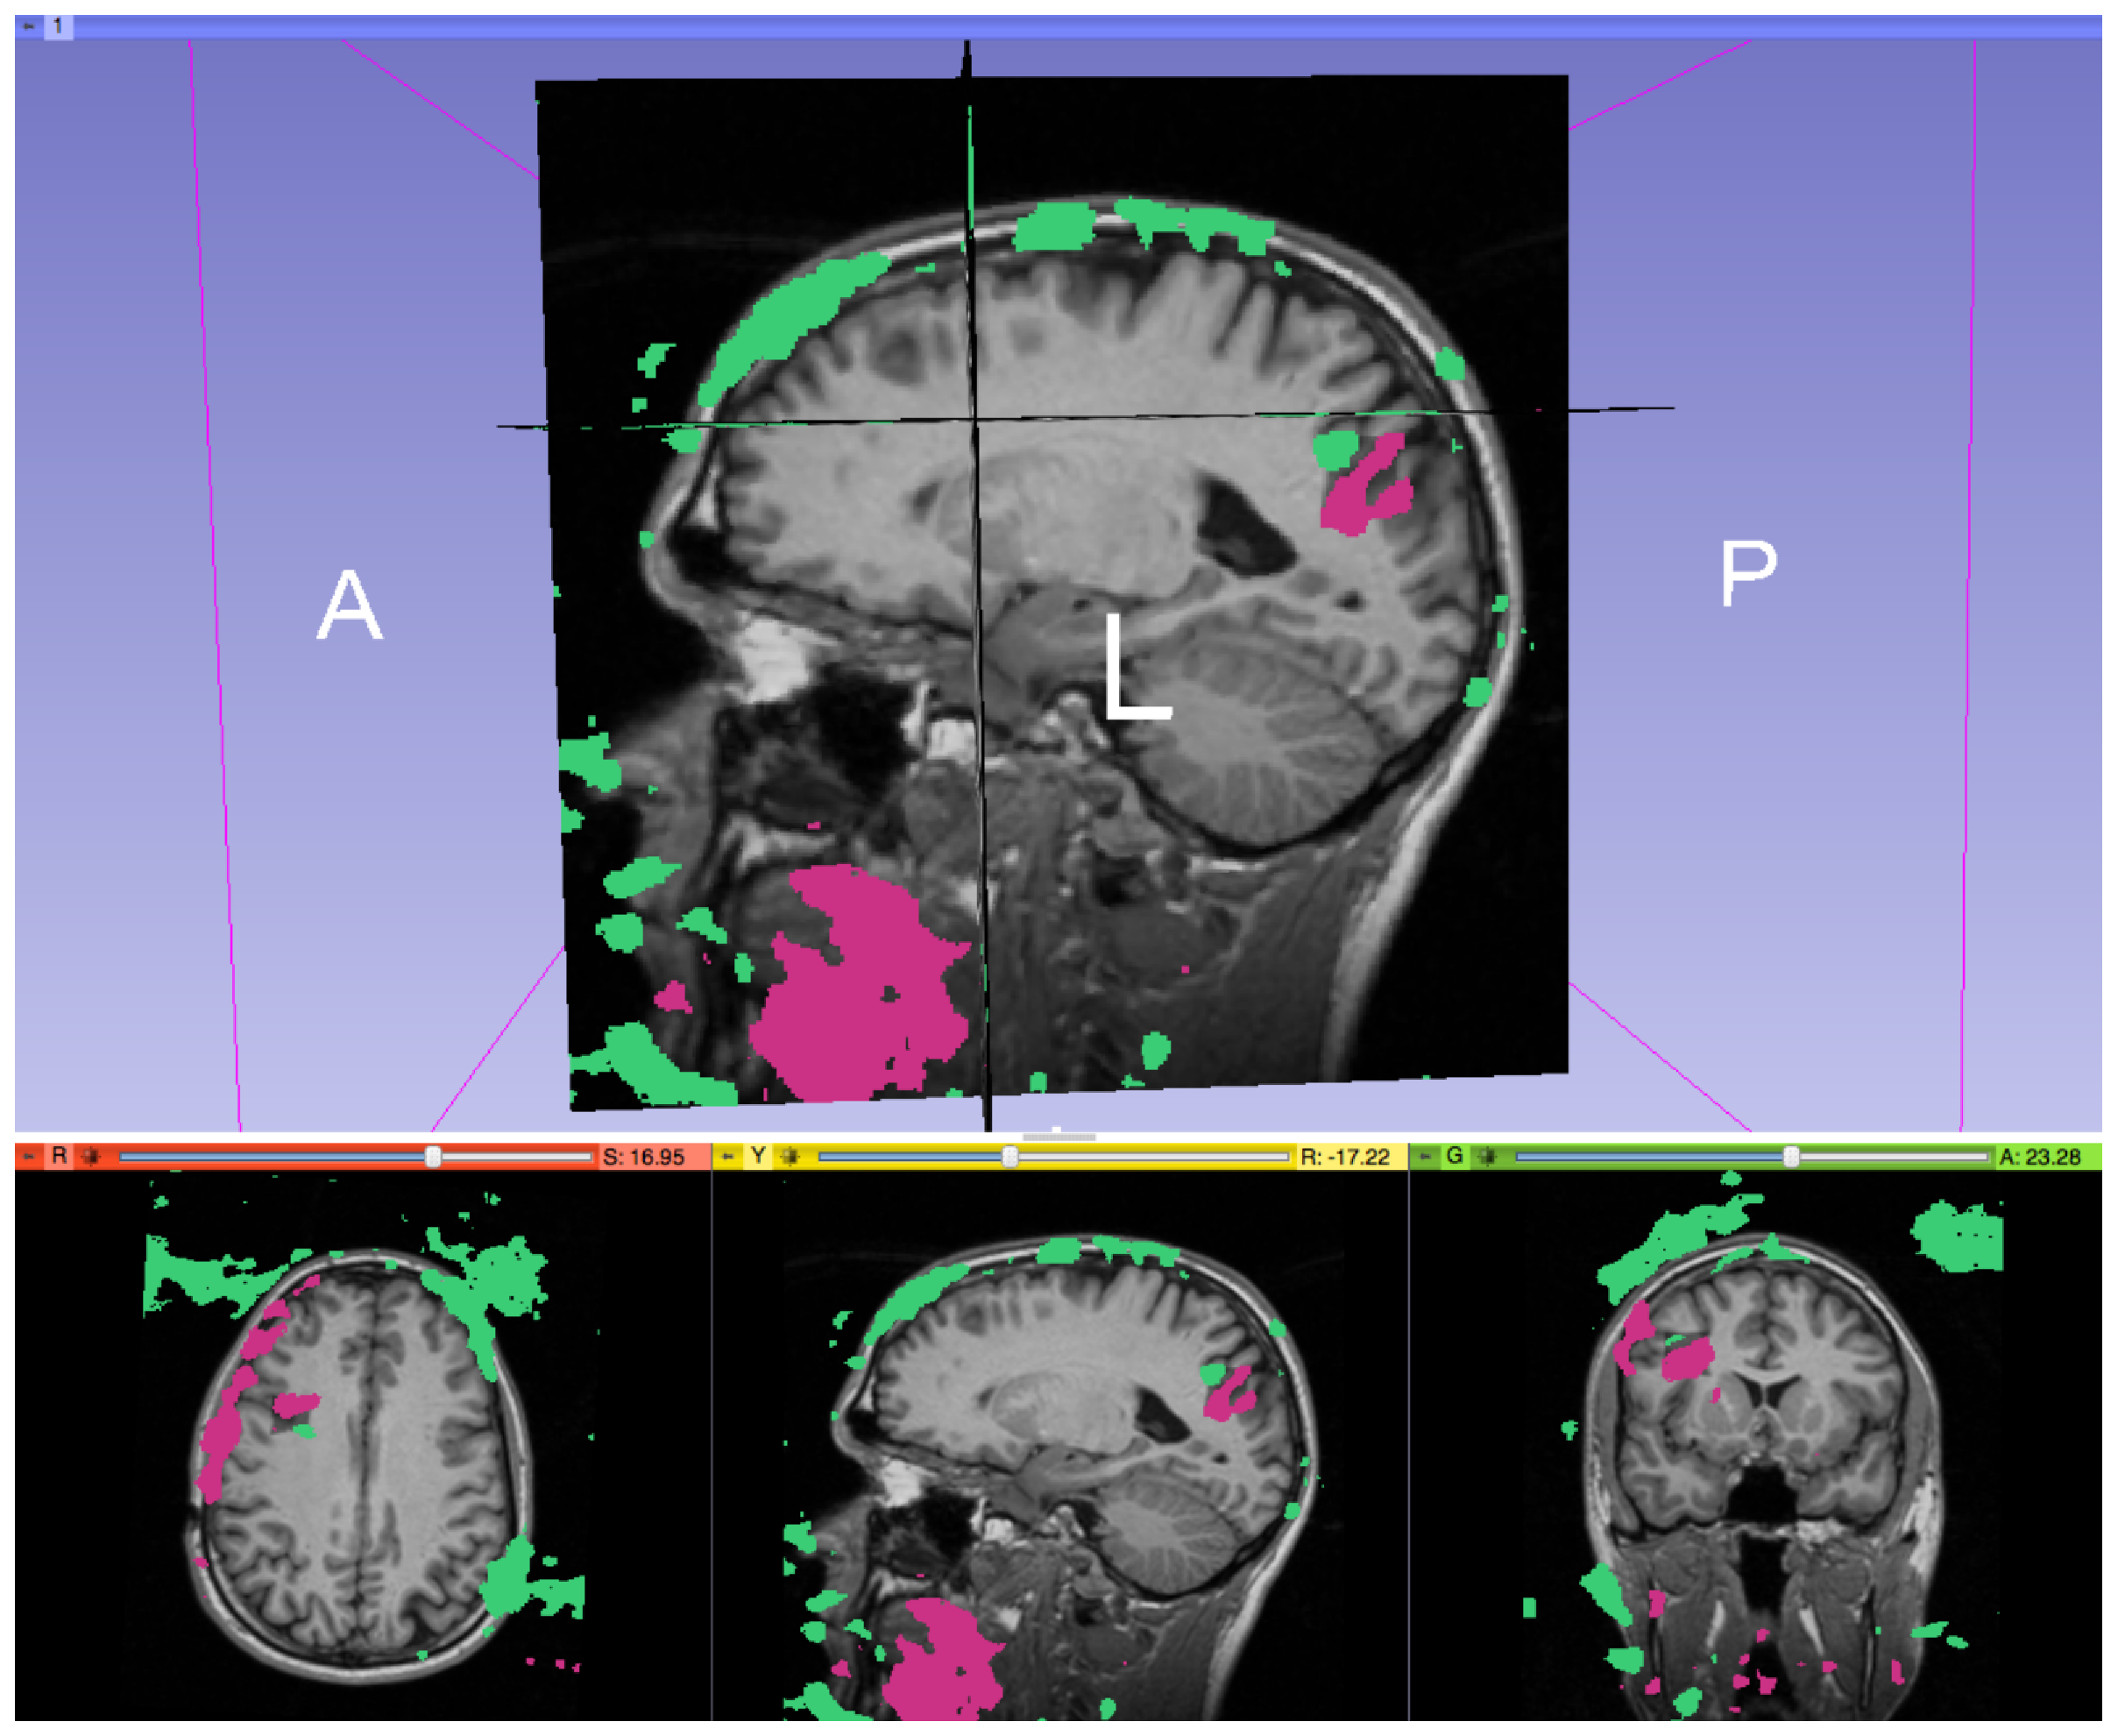
\includegraphics[scale=0.2]{/experiment_bigger/tensor80-65_bigger1.eps}
  \caption{Artificial Large: Tensor-base method}
  \label{tensor_large1}
\end{figure}

Another angle of the result:

\begin{figure}[H]
  \centering
  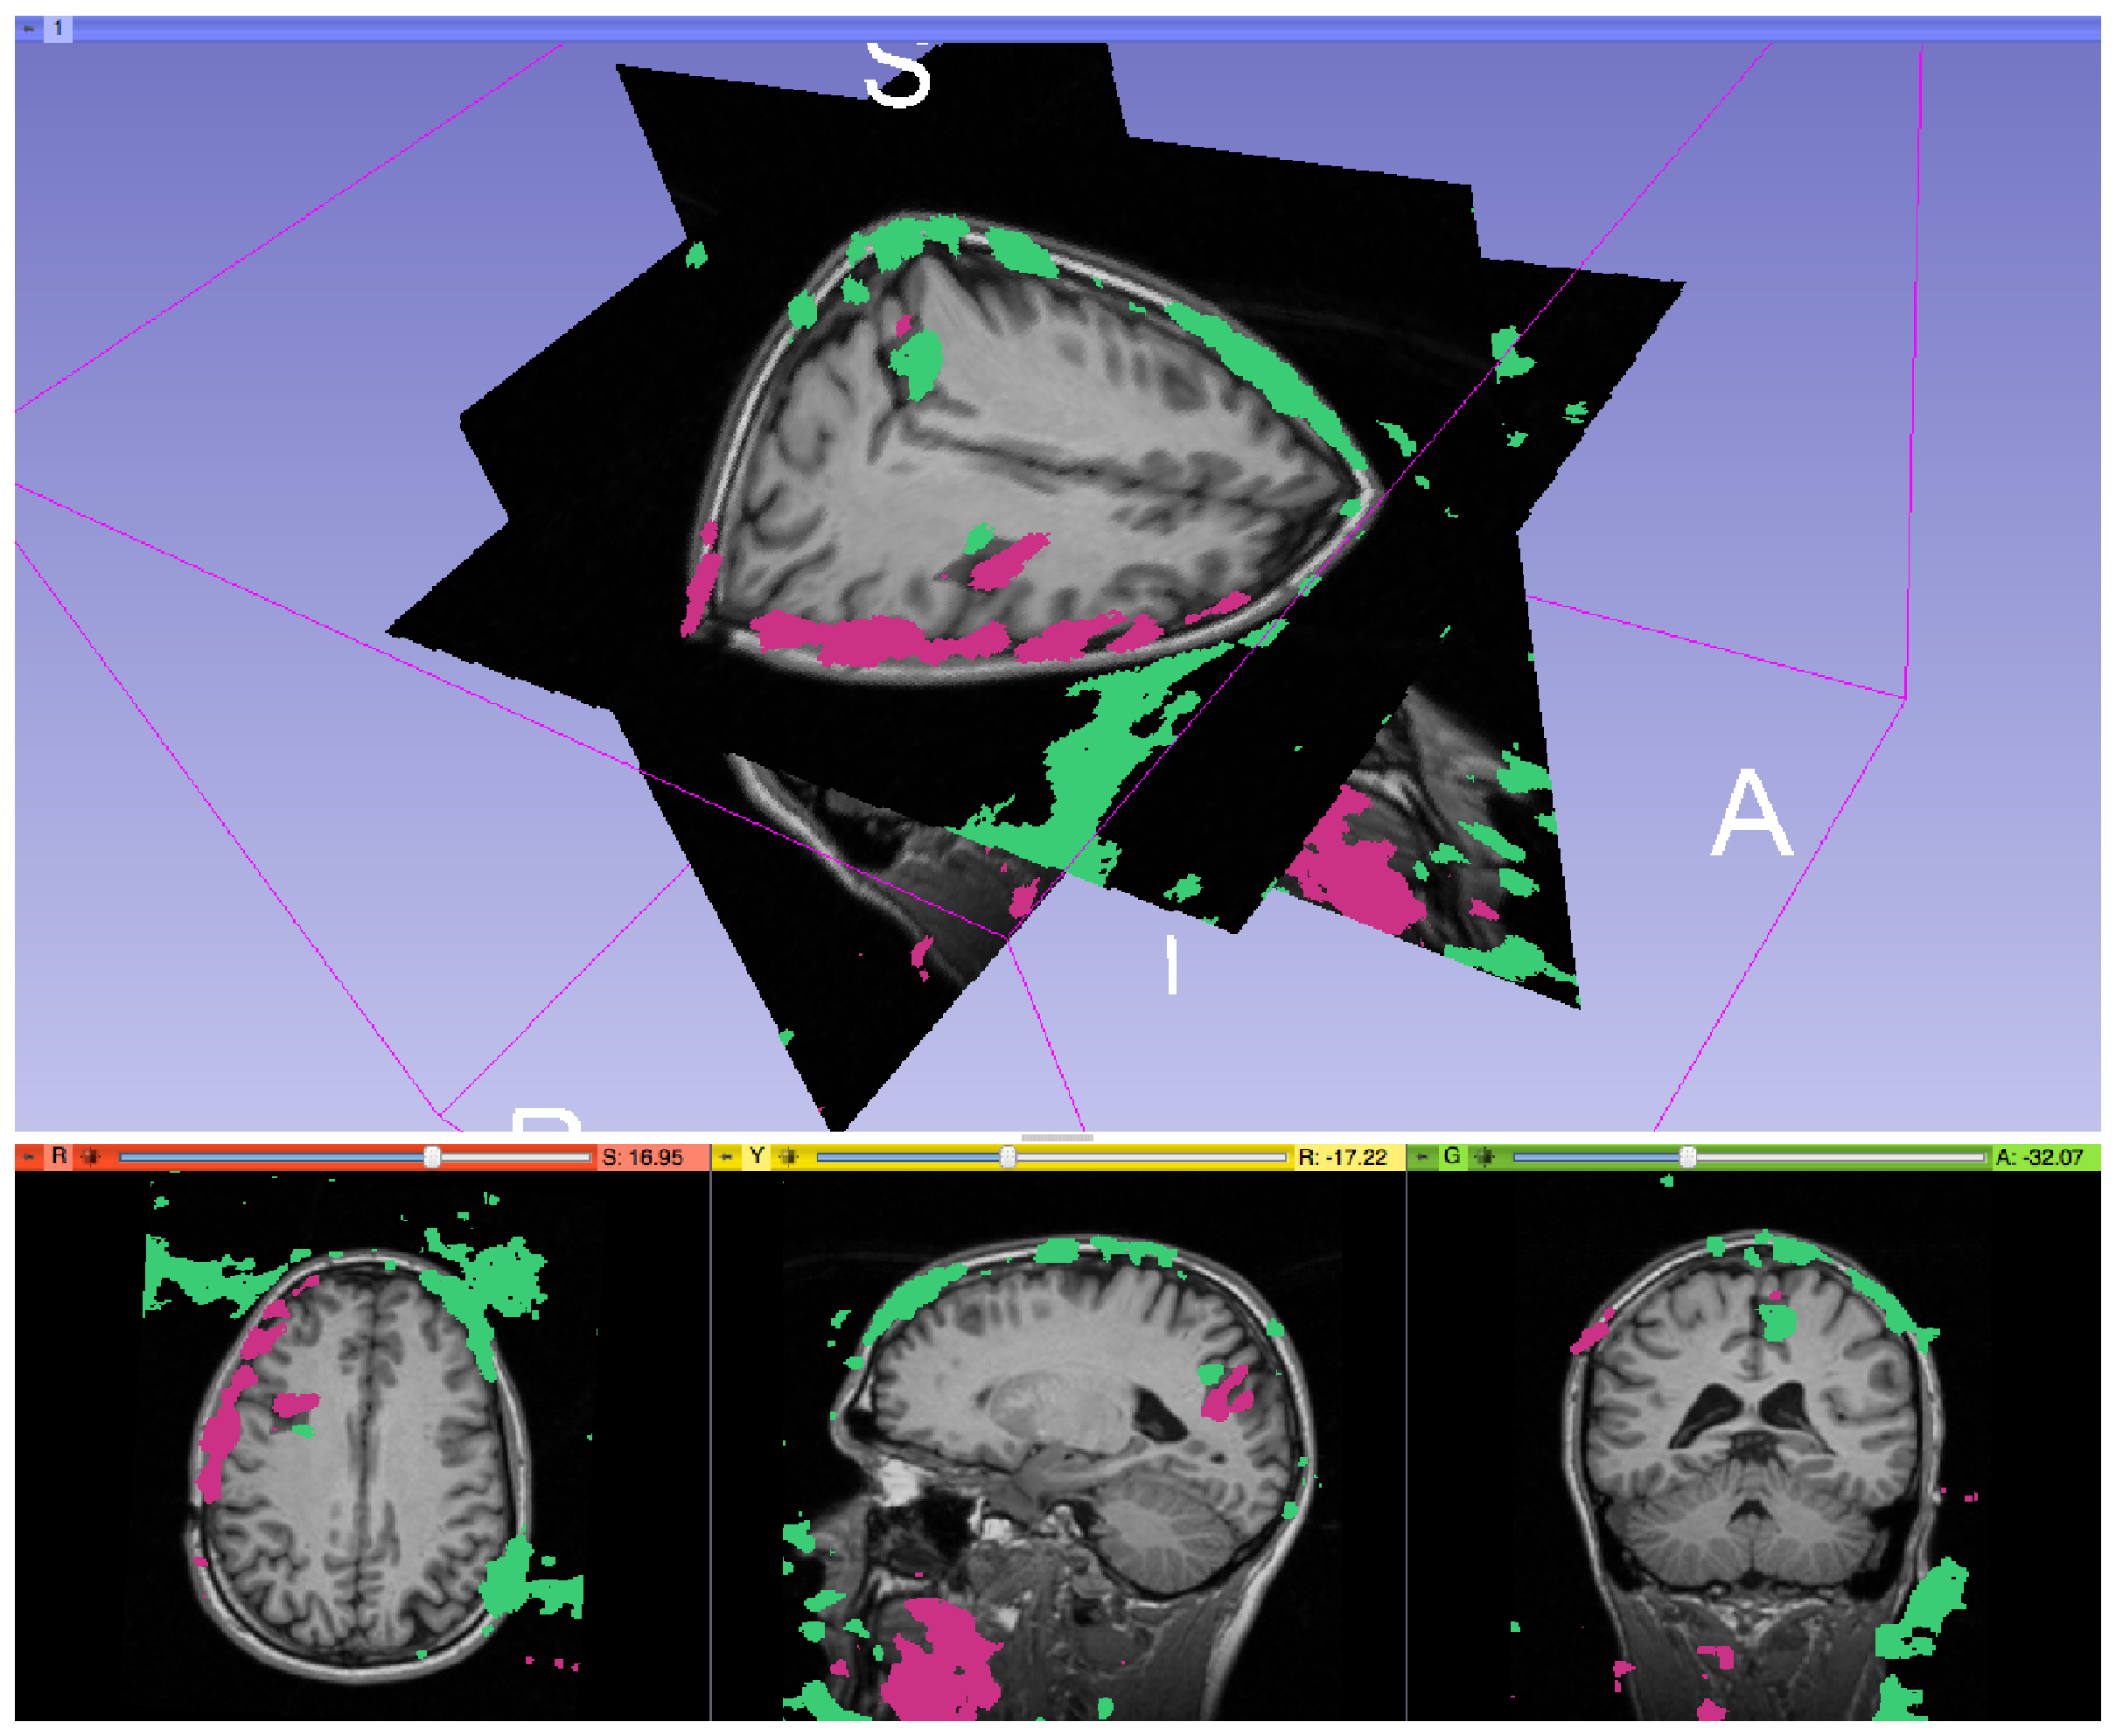
\includegraphics[scale=0.2]{/experiment_bigger/tensor80_65_bigger2.eps}
  \caption{Artificial Large: Tensor-base method}
  \label{tensor_large2}
\end{figure}


\subsection{Size: Medium}
Cubes of medium size where deleted from the follow-up volume to
represent areas of volume loss. The following volume was obtained:

\begin{figure}[H]
  \centering
  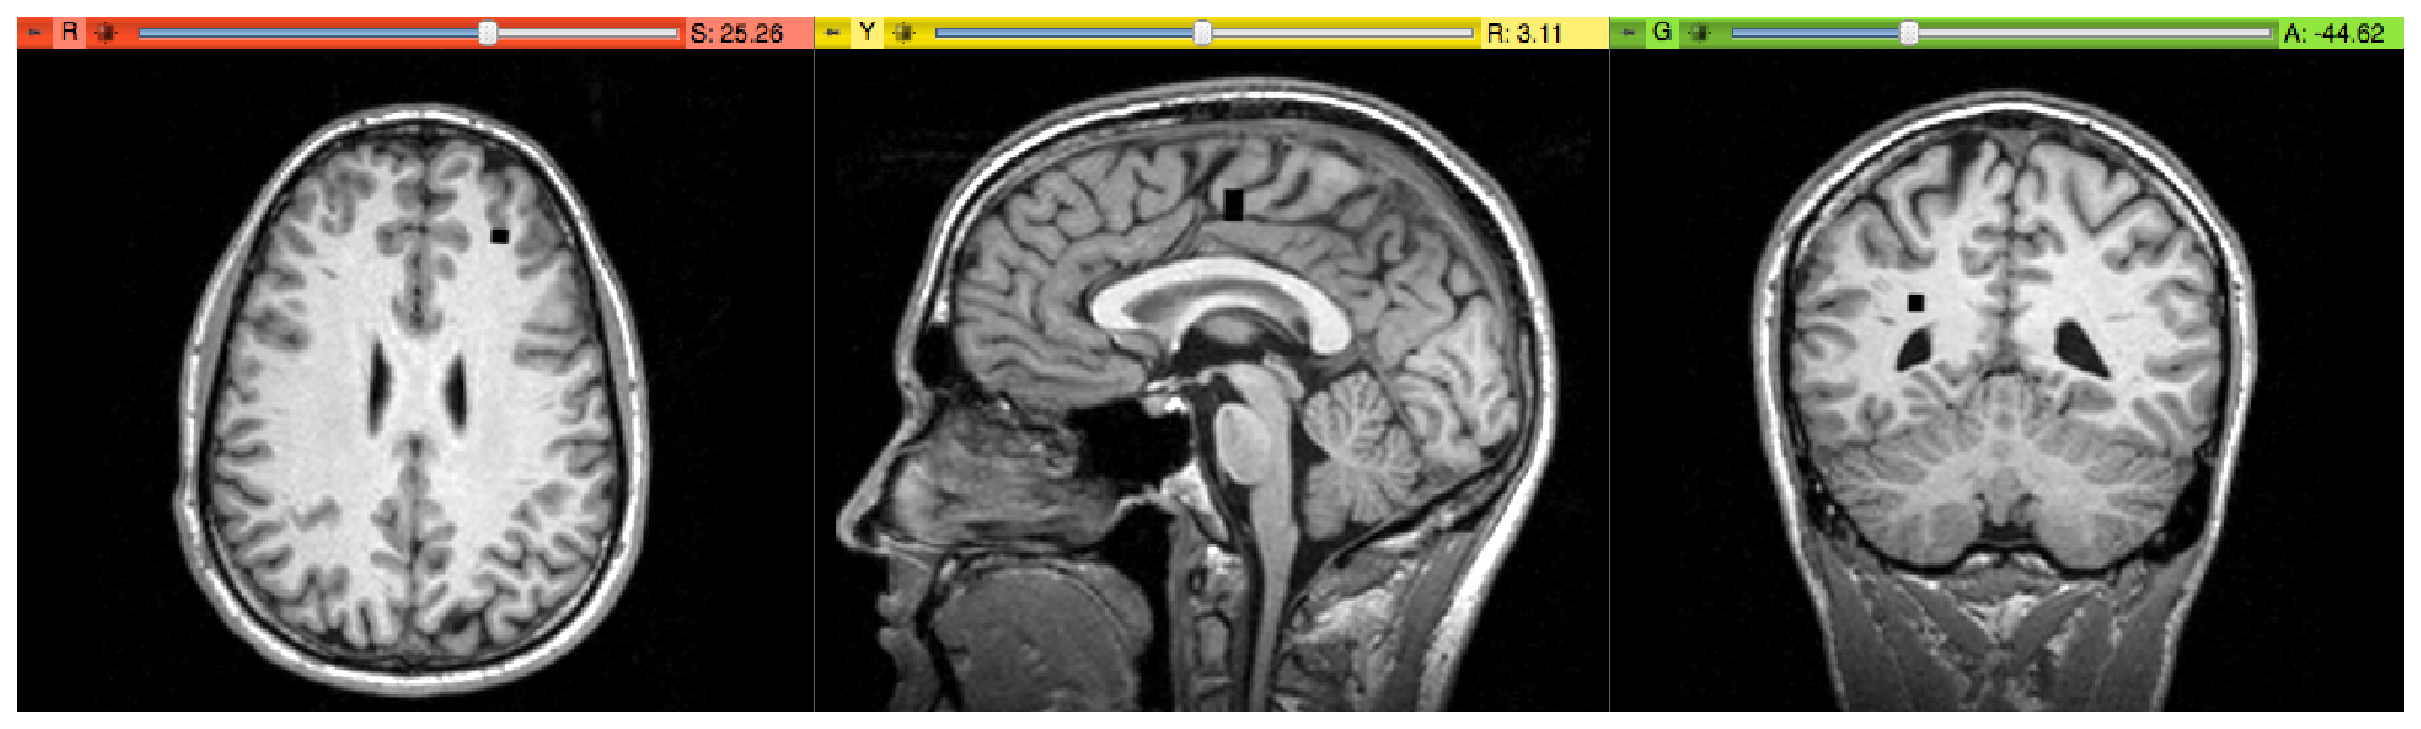
\includegraphics[scale=0.3]{/experiment_medium/medB_subtracted.eps}
  \caption{Medium Differences: Modified Follow-up volume}
  \label{largeB}
\end{figure}

\subsubsection{Voxel-based Method}
The result obtained with this method and medium differences is as good
as with larger differences. All the deleted volume cubes are found and
easy to see in the result.

\begin{figure}[H]
  \centering
  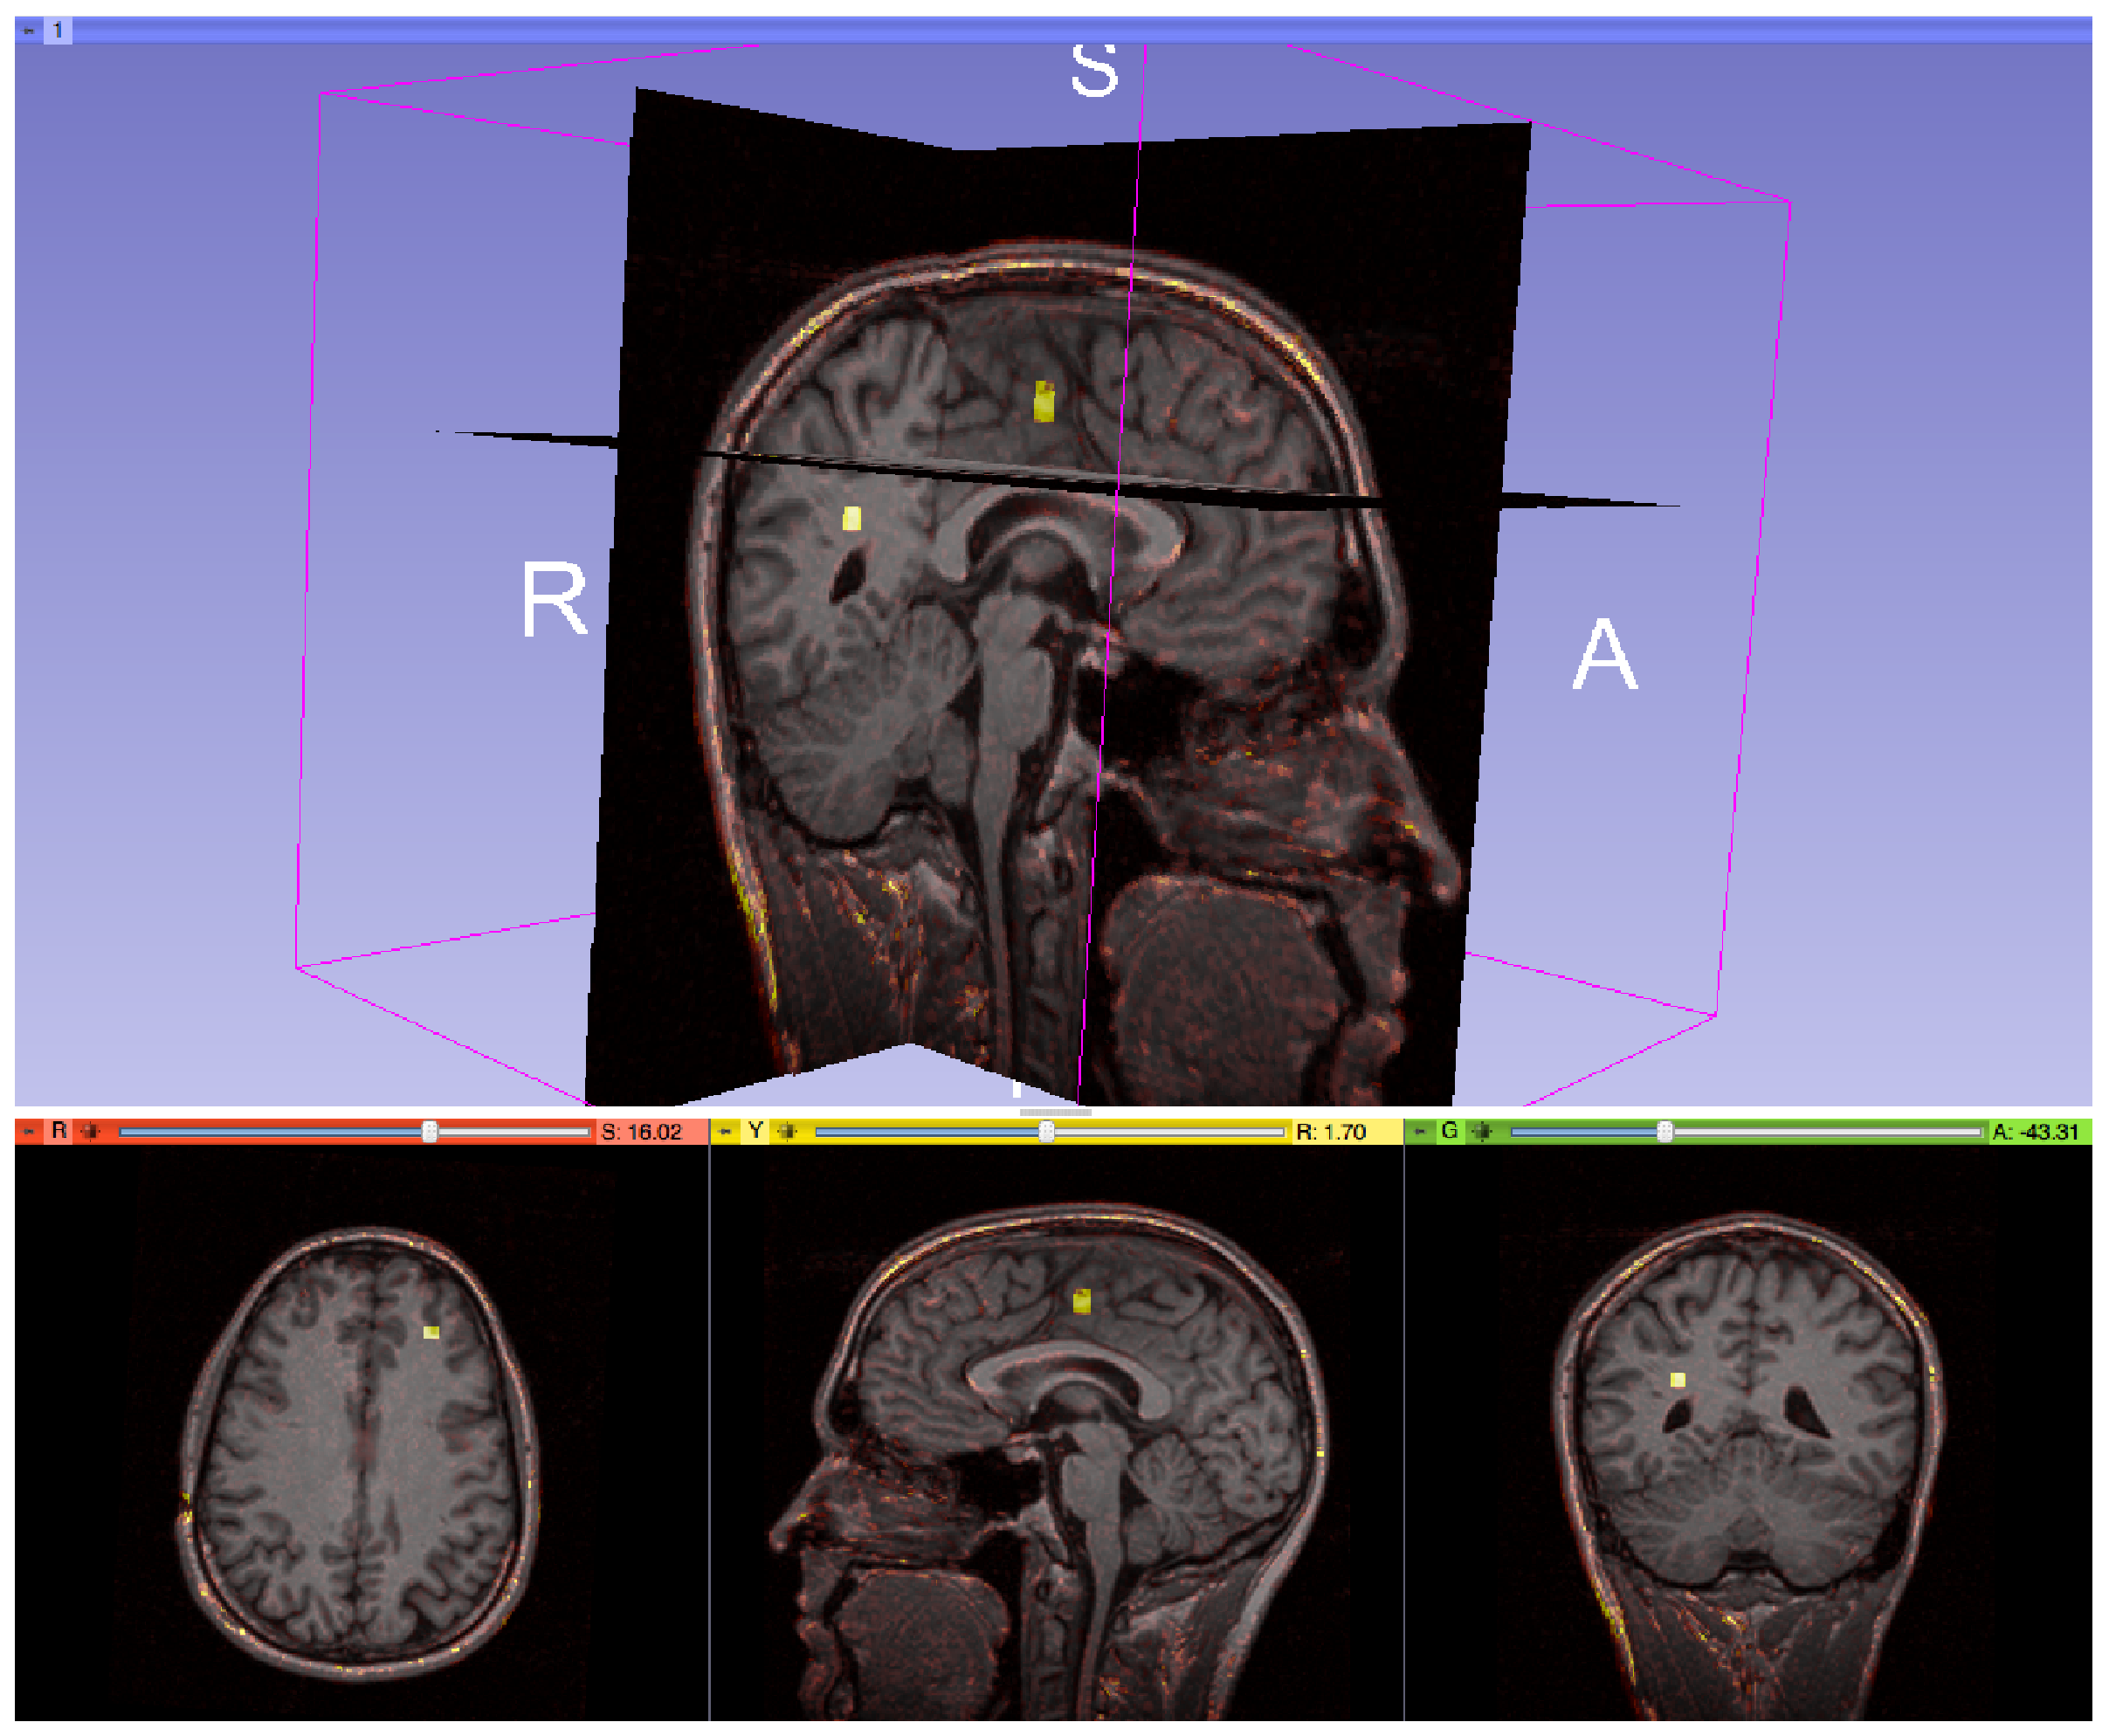
\includegraphics[scale=0.2]{/experiment_medium/med_voxel1.eps}
  \caption{Artificial Medium: Voxel-base method}
  \label{voxel_med1}
\end{figure}

Another angle of the result:

\begin{figure}[H]
  \centering
  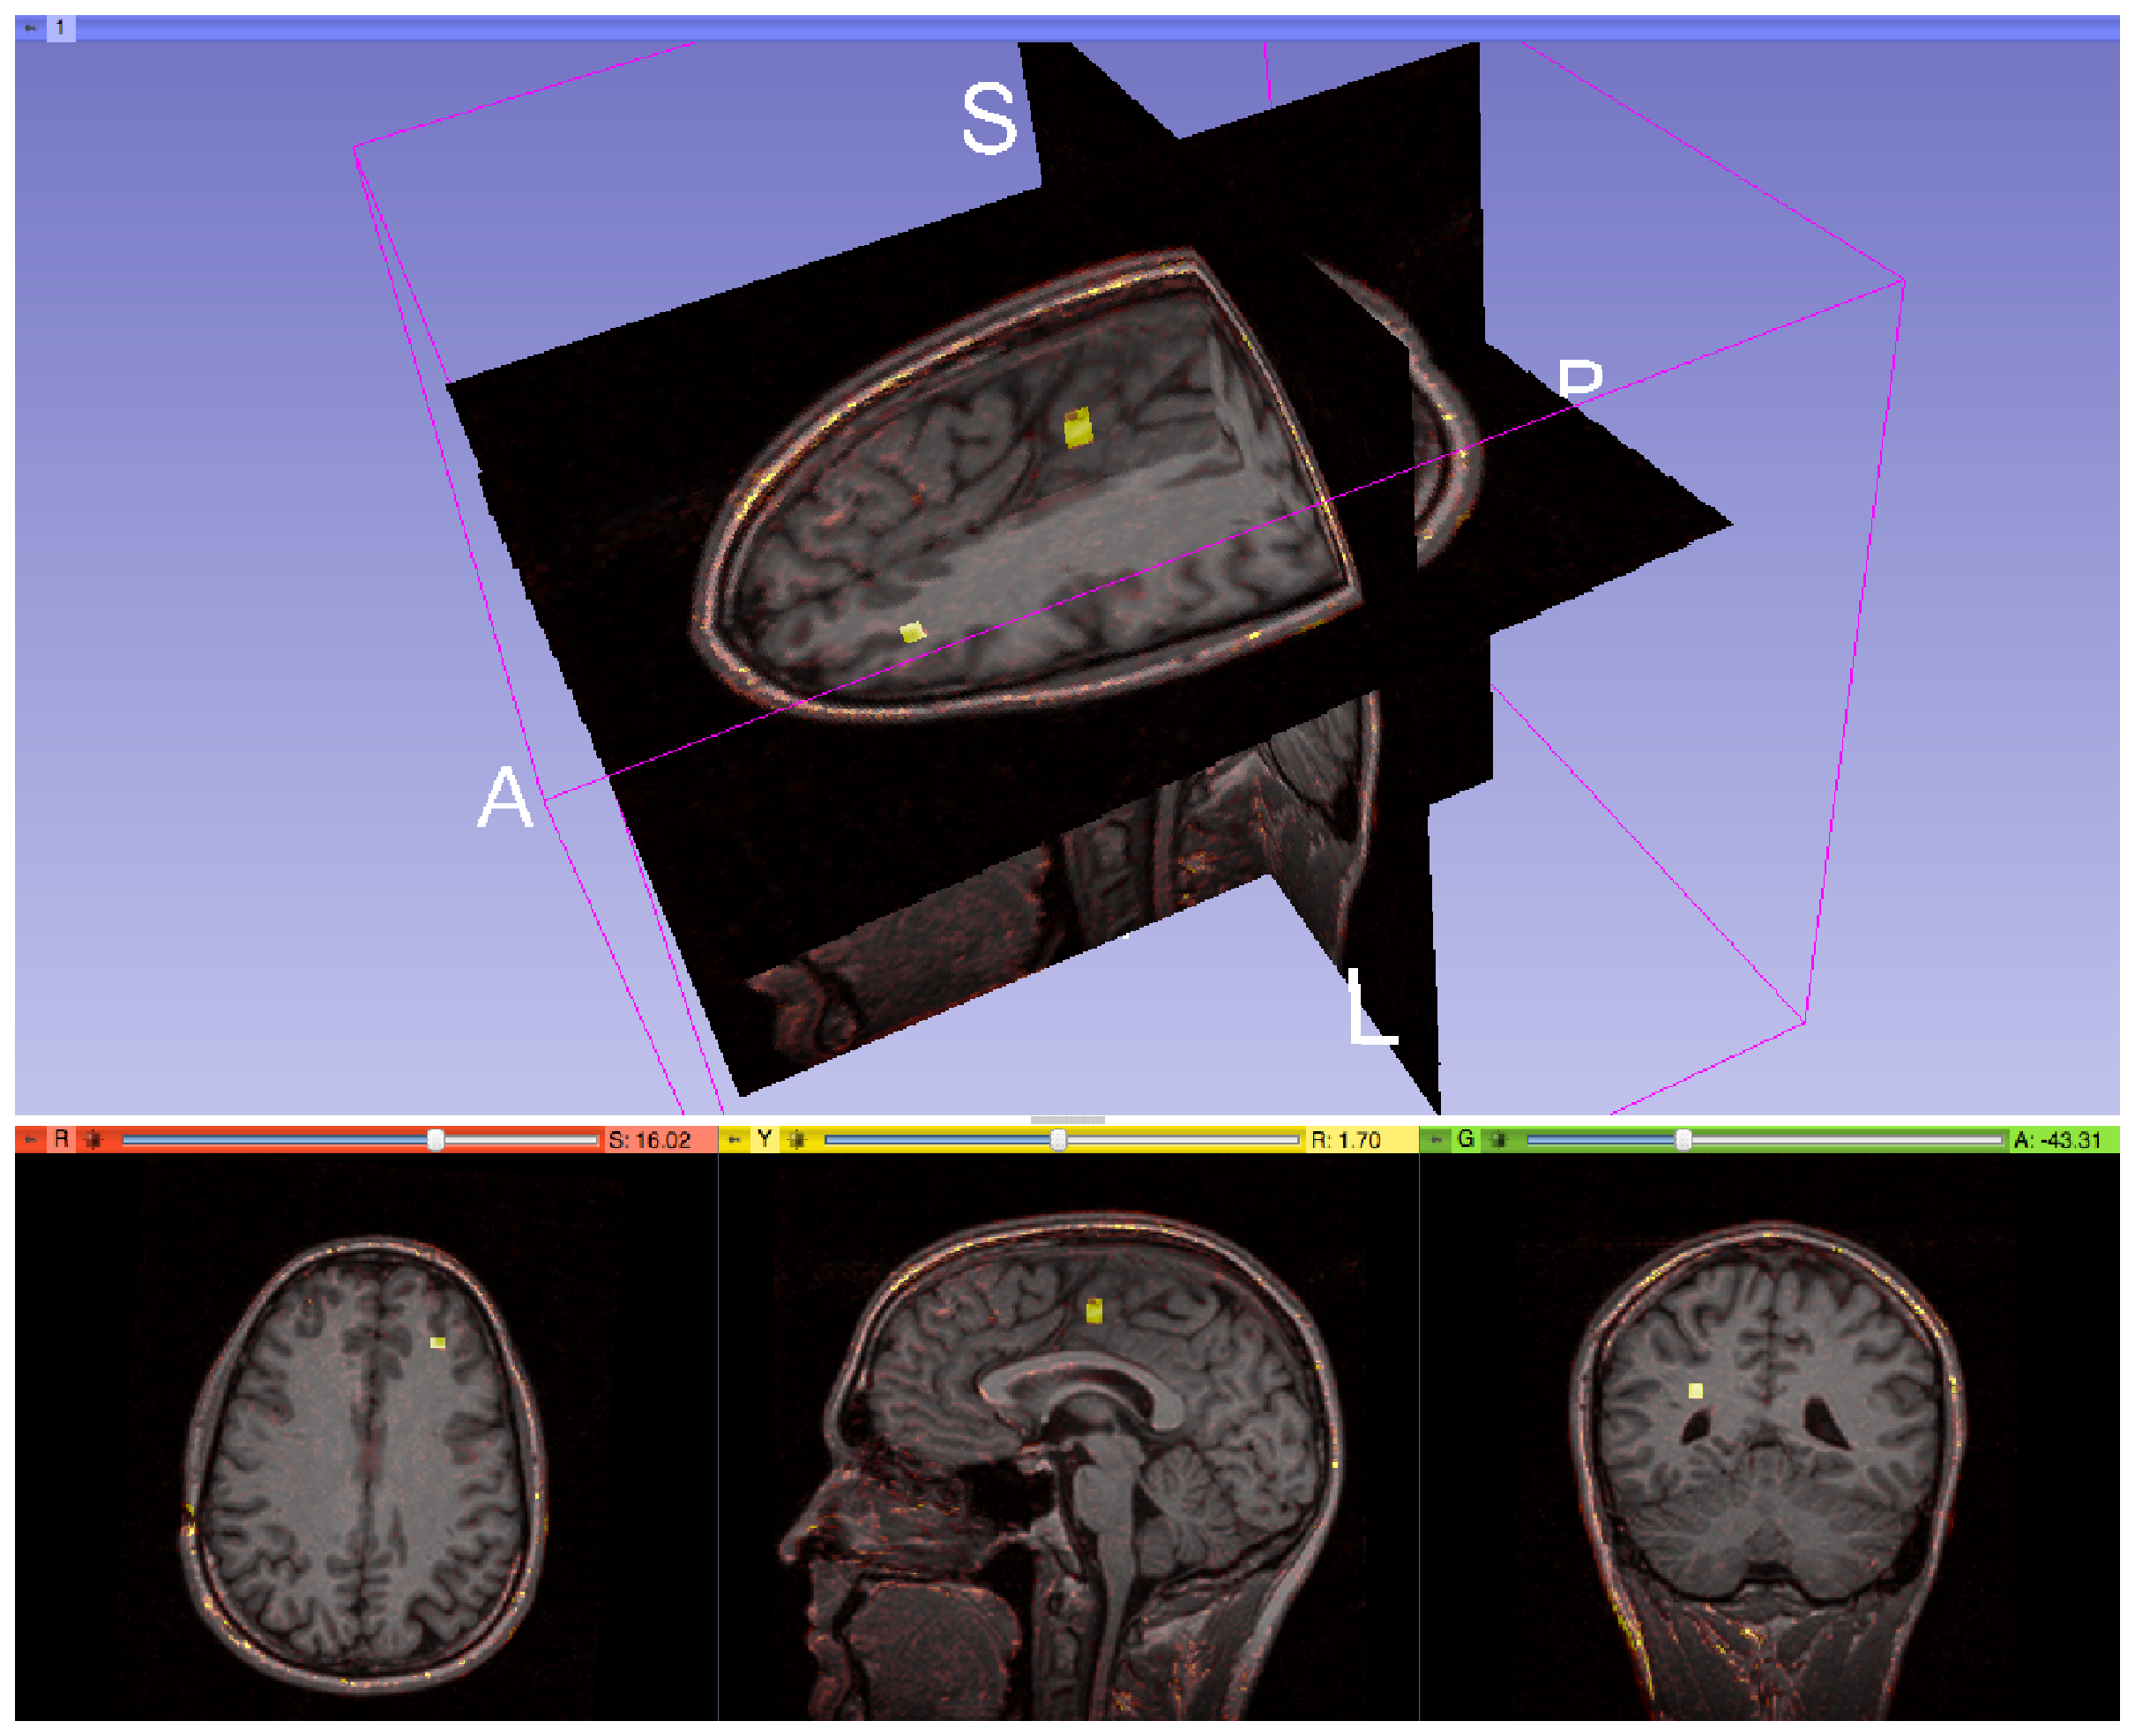
\includegraphics[scale=0.2]{/experiment_medium/med_voxel2.eps}
  \caption{Artificial Medium: Voxel-base method}
  \label{voxel_med2}
\end{figure}

\subsubsection{Tensor-based Method}
The result is a bit worse than for bigger differences. The volume
losses are still found by the application, but their borders are not
defined and the method also founds other zones with differences that
are hard to differenciate from the added ones.

The parameters used to obtain this result are:
\begin{description}
\item \textit{Deformation field smoothing sigma:} 2.5
\item \textit{Shrinkage percentage:} 80
\item \textit{Growth percentage:} 76
\end{description}

\begin{figure}[H]
  \centering
  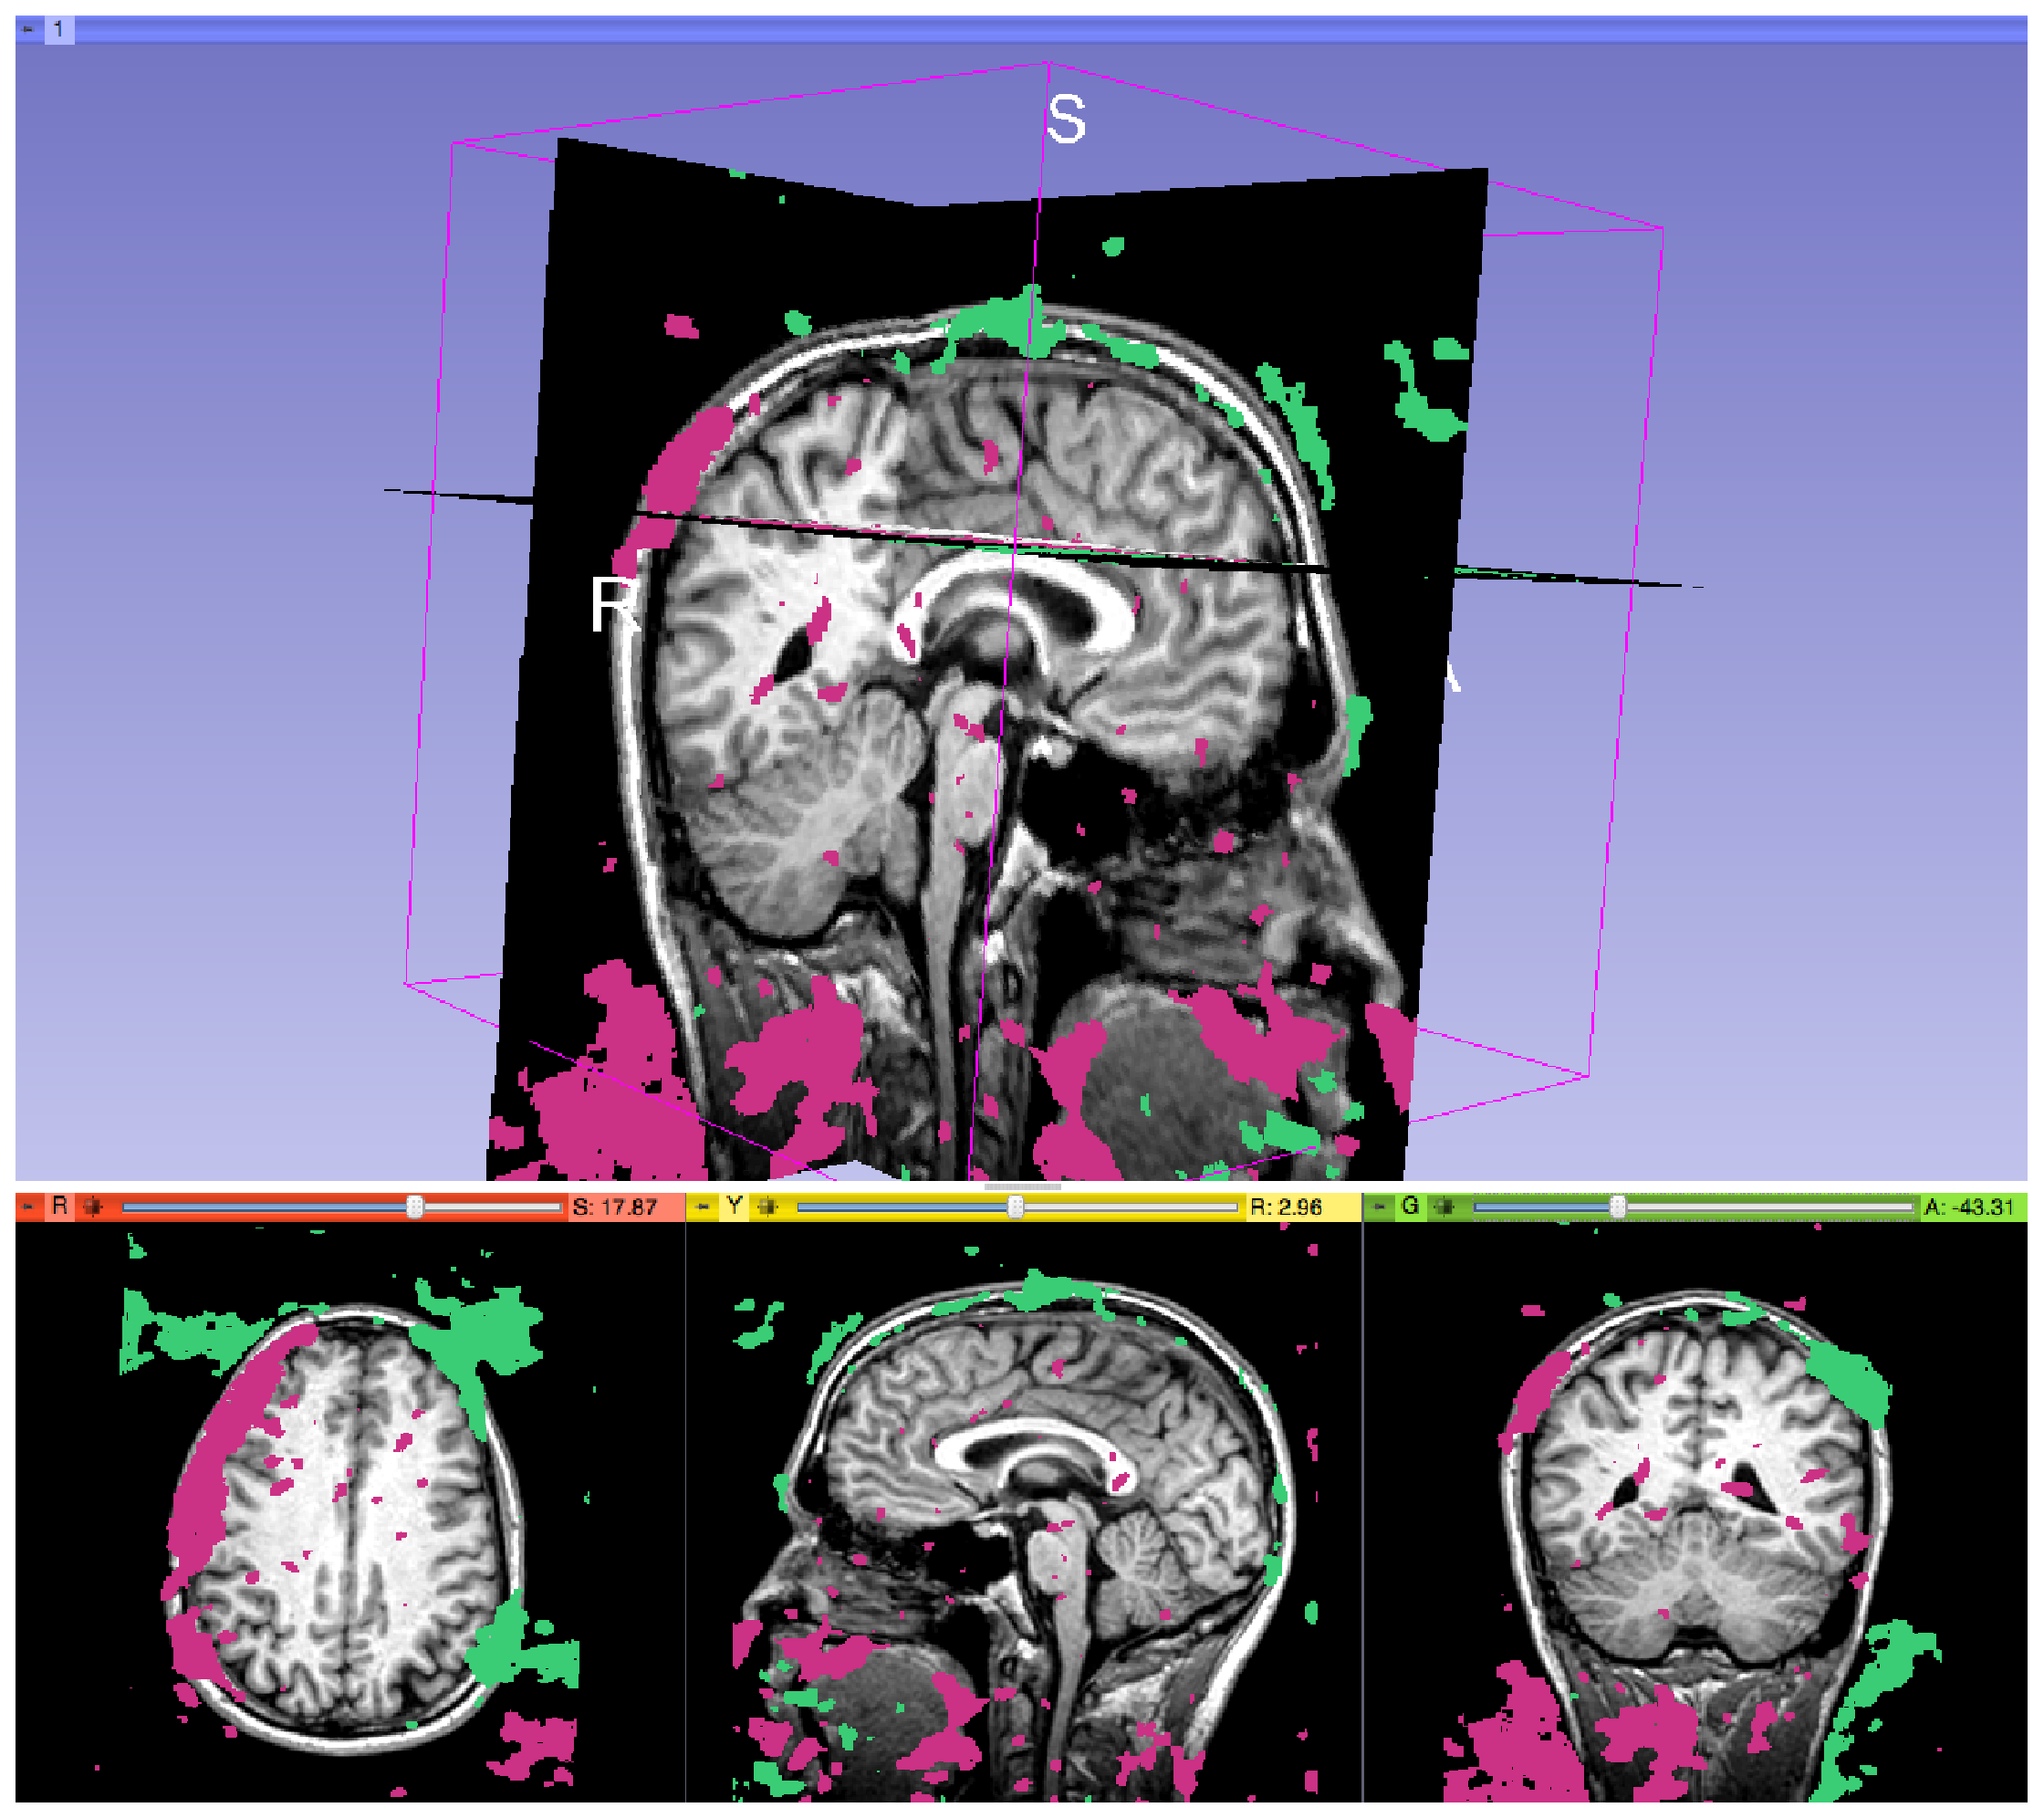
\includegraphics[scale=0.2]{/experiment_medium/tensor80-76_med1.eps}
  \caption{Artificial Medium: Tensor-base method}
  \label{tensor_med1}
\end{figure}

Another angle of the result:

\begin{figure}[H]
  \centering
  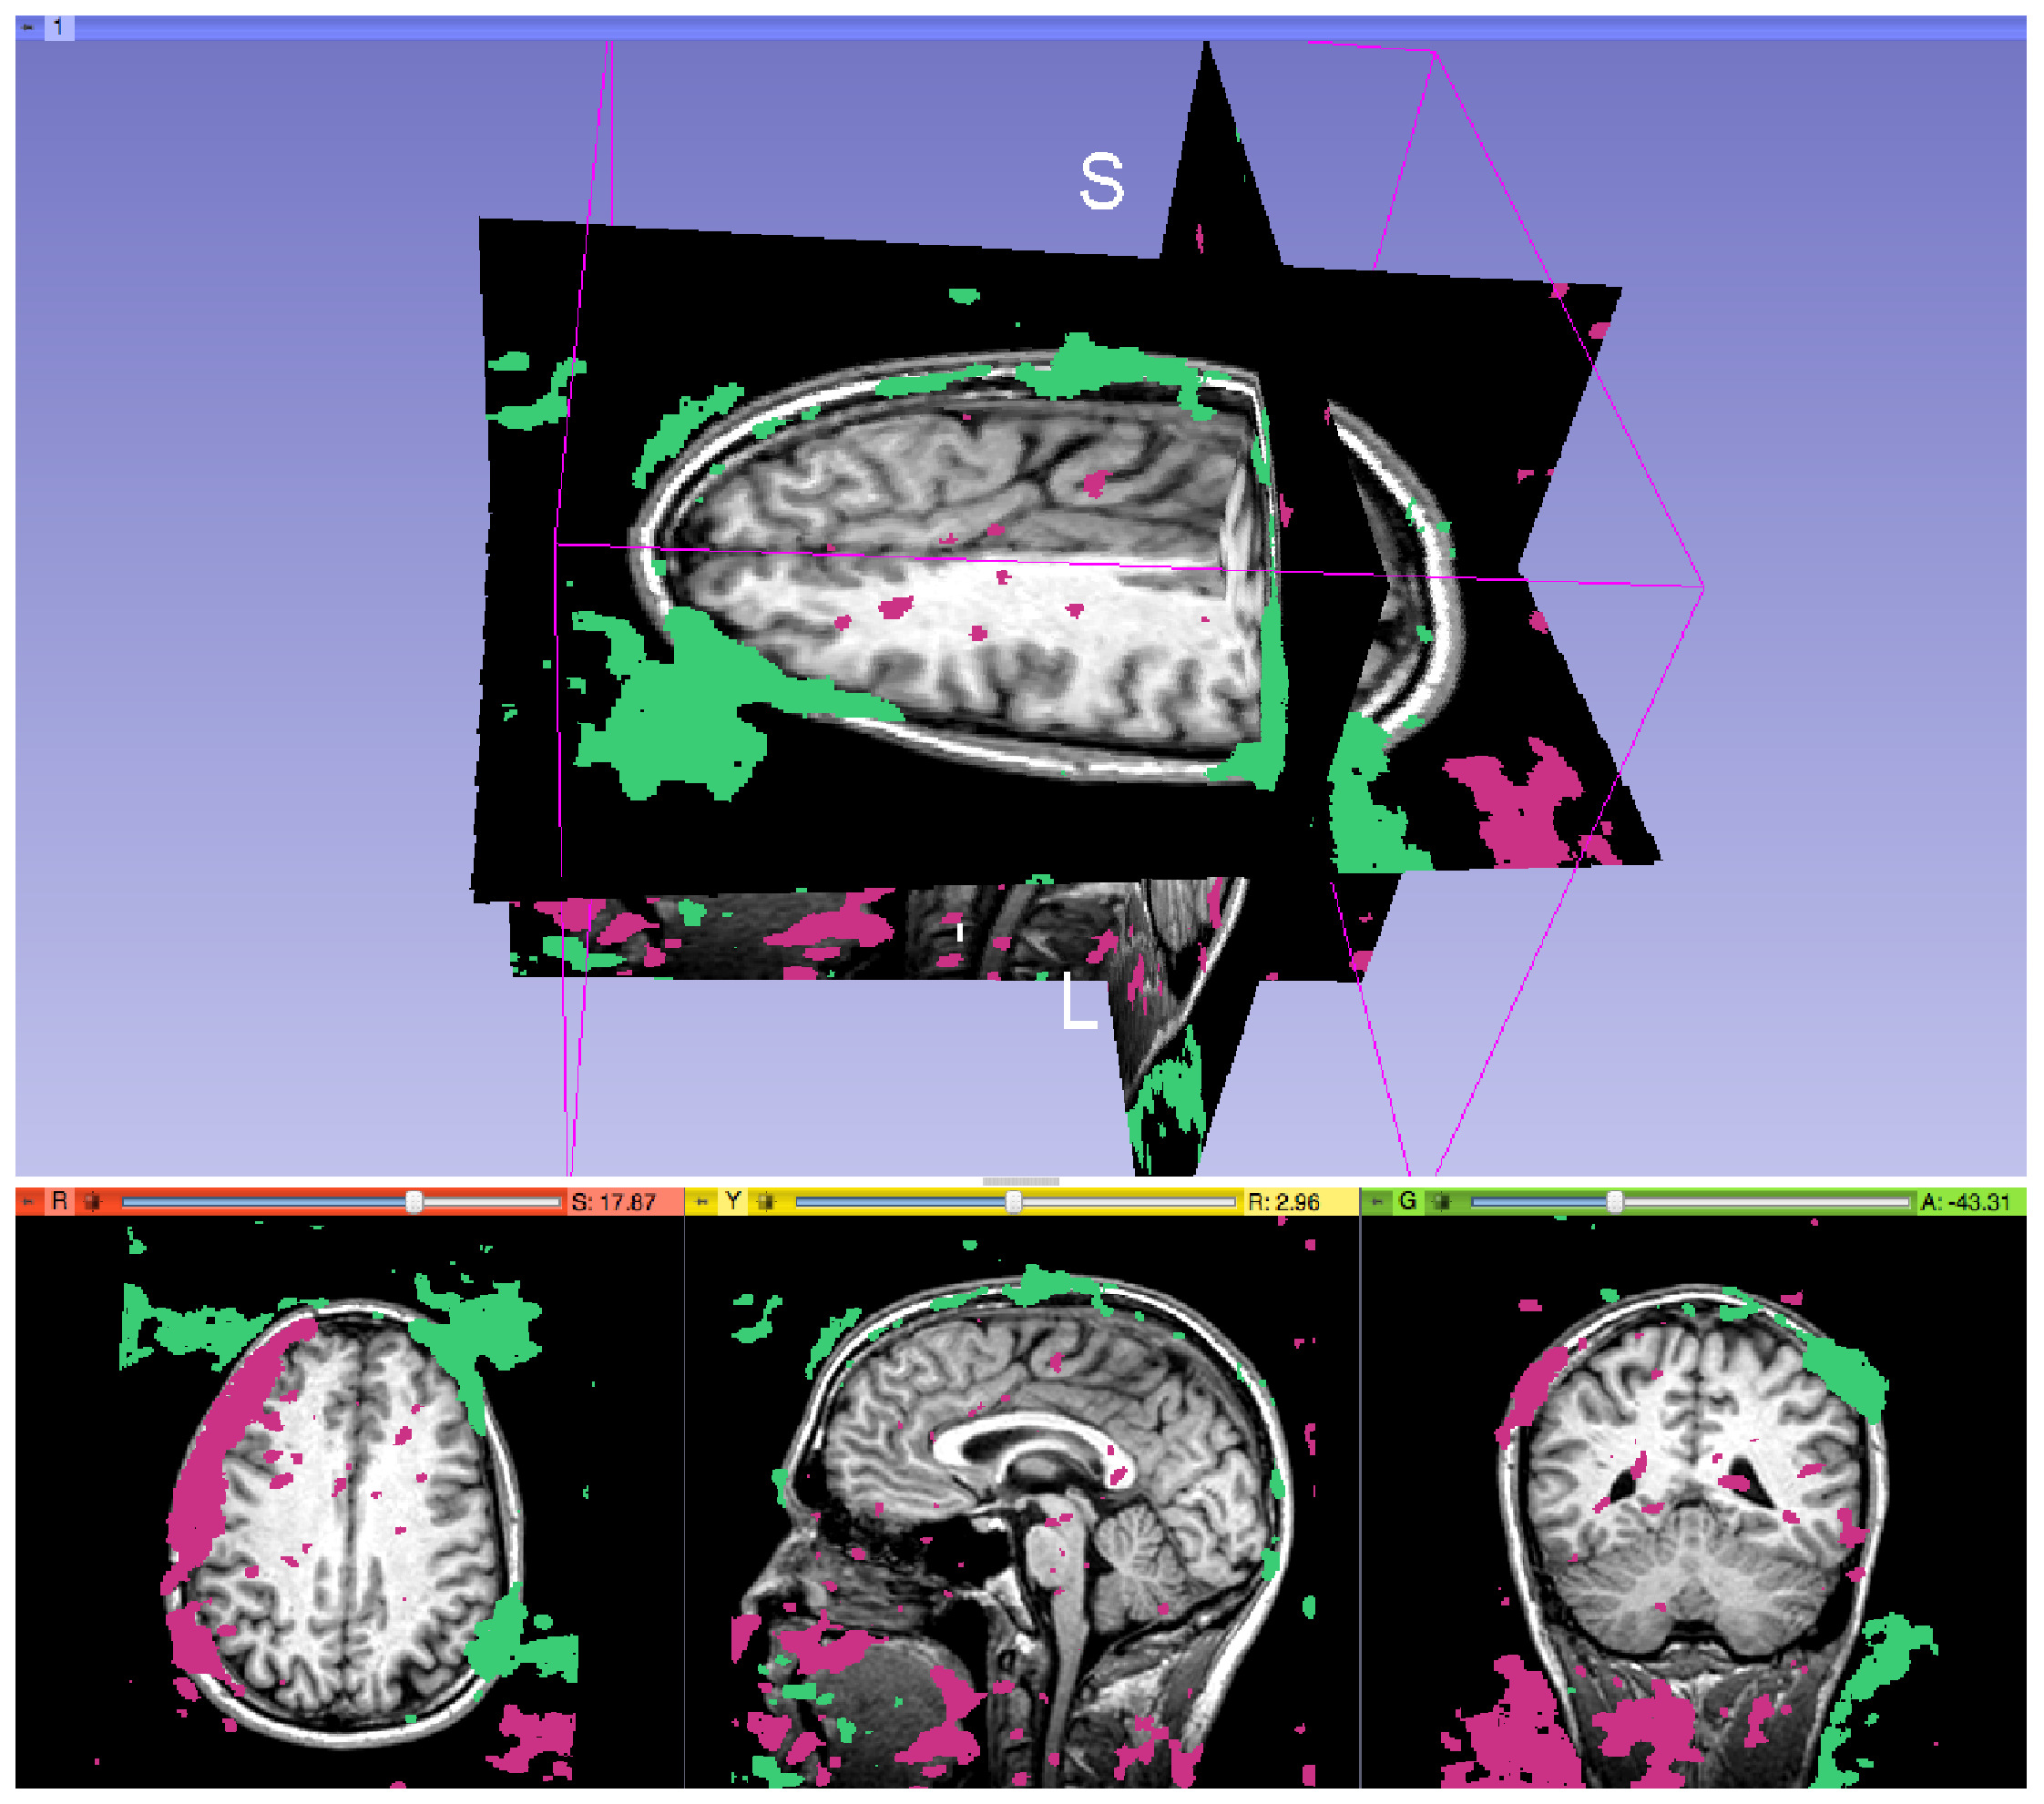
\includegraphics[scale=0.2]{/experiment_medium/tensor80-76_med2.eps}
  \caption{Artificial Medium: Tensor-base method}
  \label{tensor_med2}
\end{figure}

\subsection{Size: Small}
Rectangles of very small size where deleted from the follow-up volume
to represent areas of volume loss. Rectangles were selected instead of
cubes in this case in order to be able to view the result more simply.

The following volume was obtained. In this image, the small rectangles
are marked in red just for the purpose of being more visible in this
report. The original image does not include the red circles:

\begin{figure}[H]
  \centering
  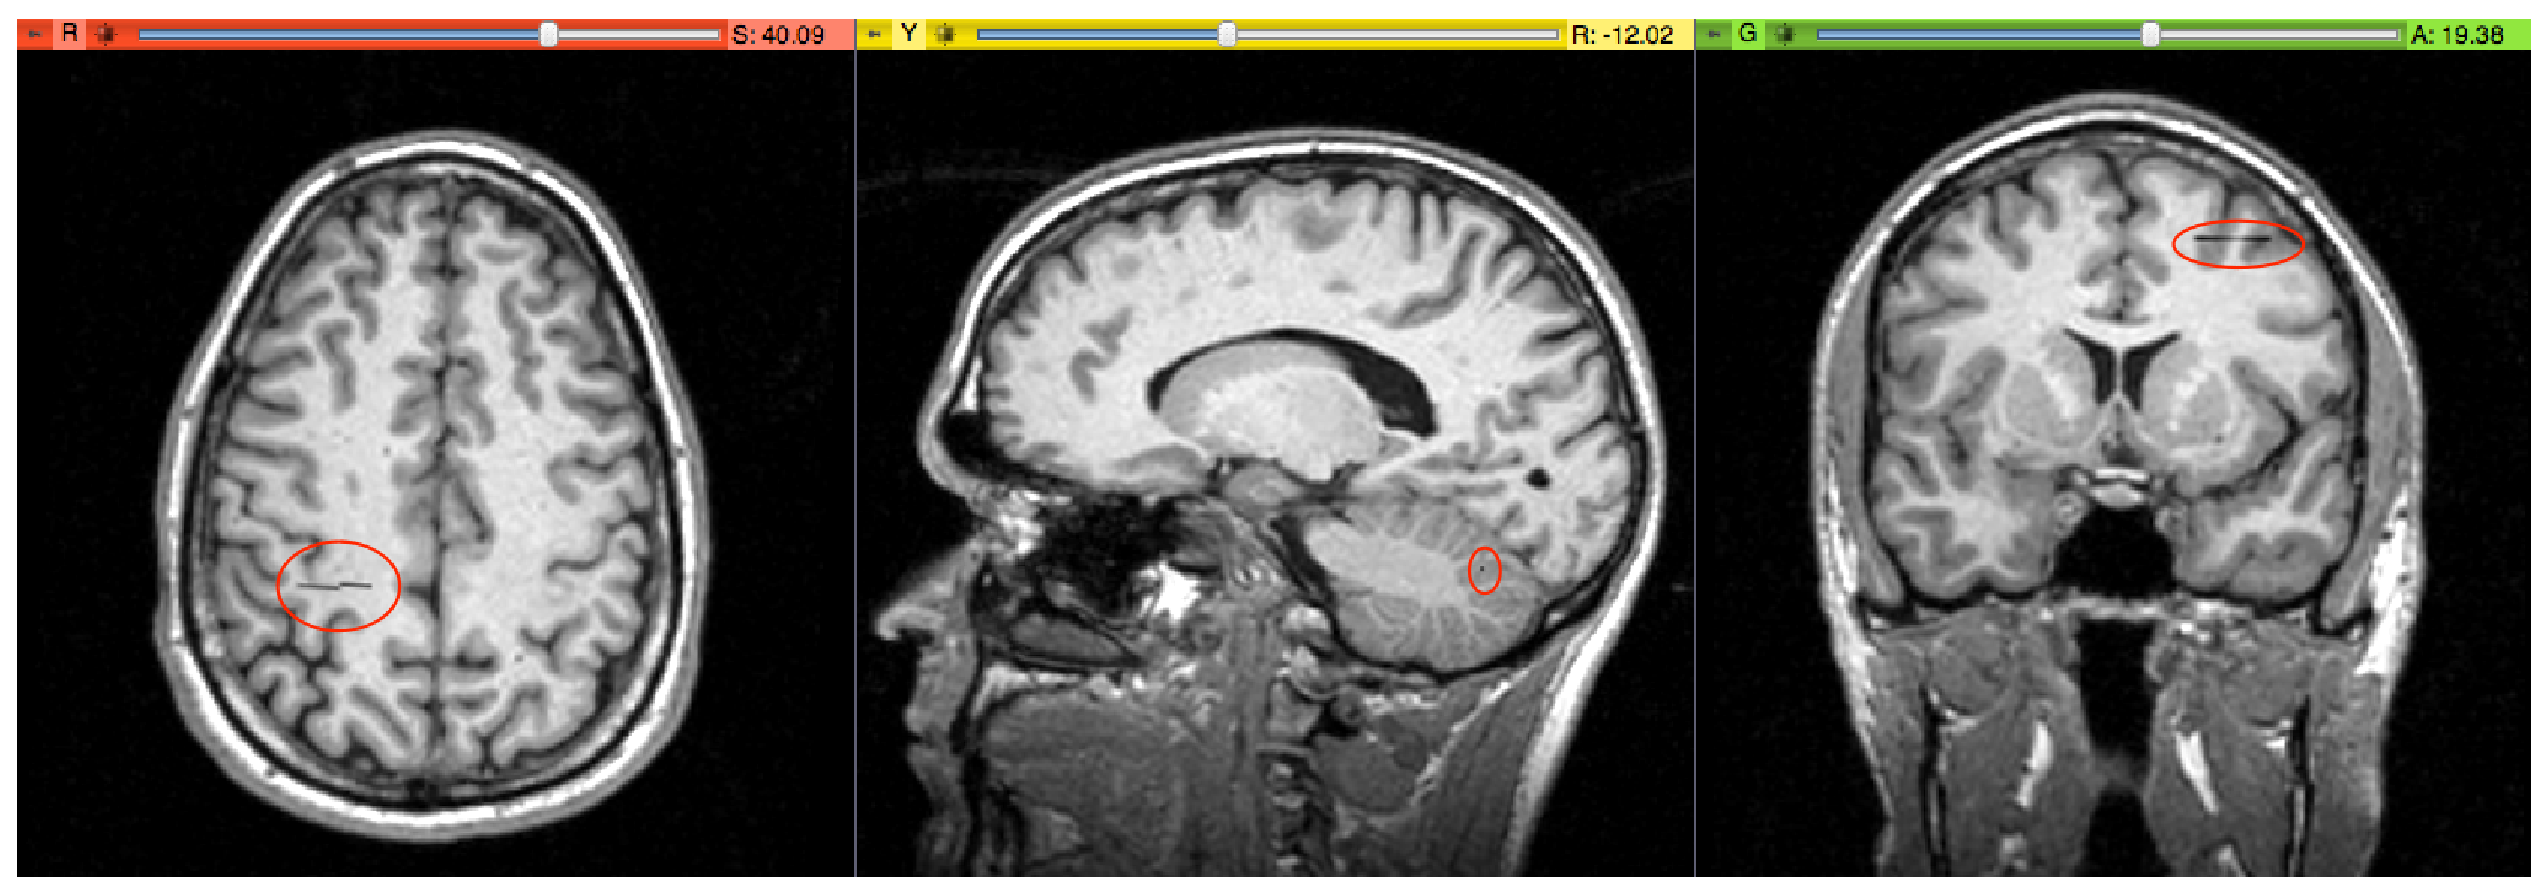
\includegraphics[scale=0.3]{/experiment_small/small_differences.eps}
  \caption{Small Differences: Modified Follow-up volume}
  \label{smallB}
\end{figure}

\subsubsection{Voxel-based Method}
The result obtained with this method and small differences is also
very good. All the deleted volume rectagles are found in the result,
although in this case the differences are so small that could be hard
to see, even when they are highlighted in the resulting volume.

\begin{figure}[H]
  \centering
  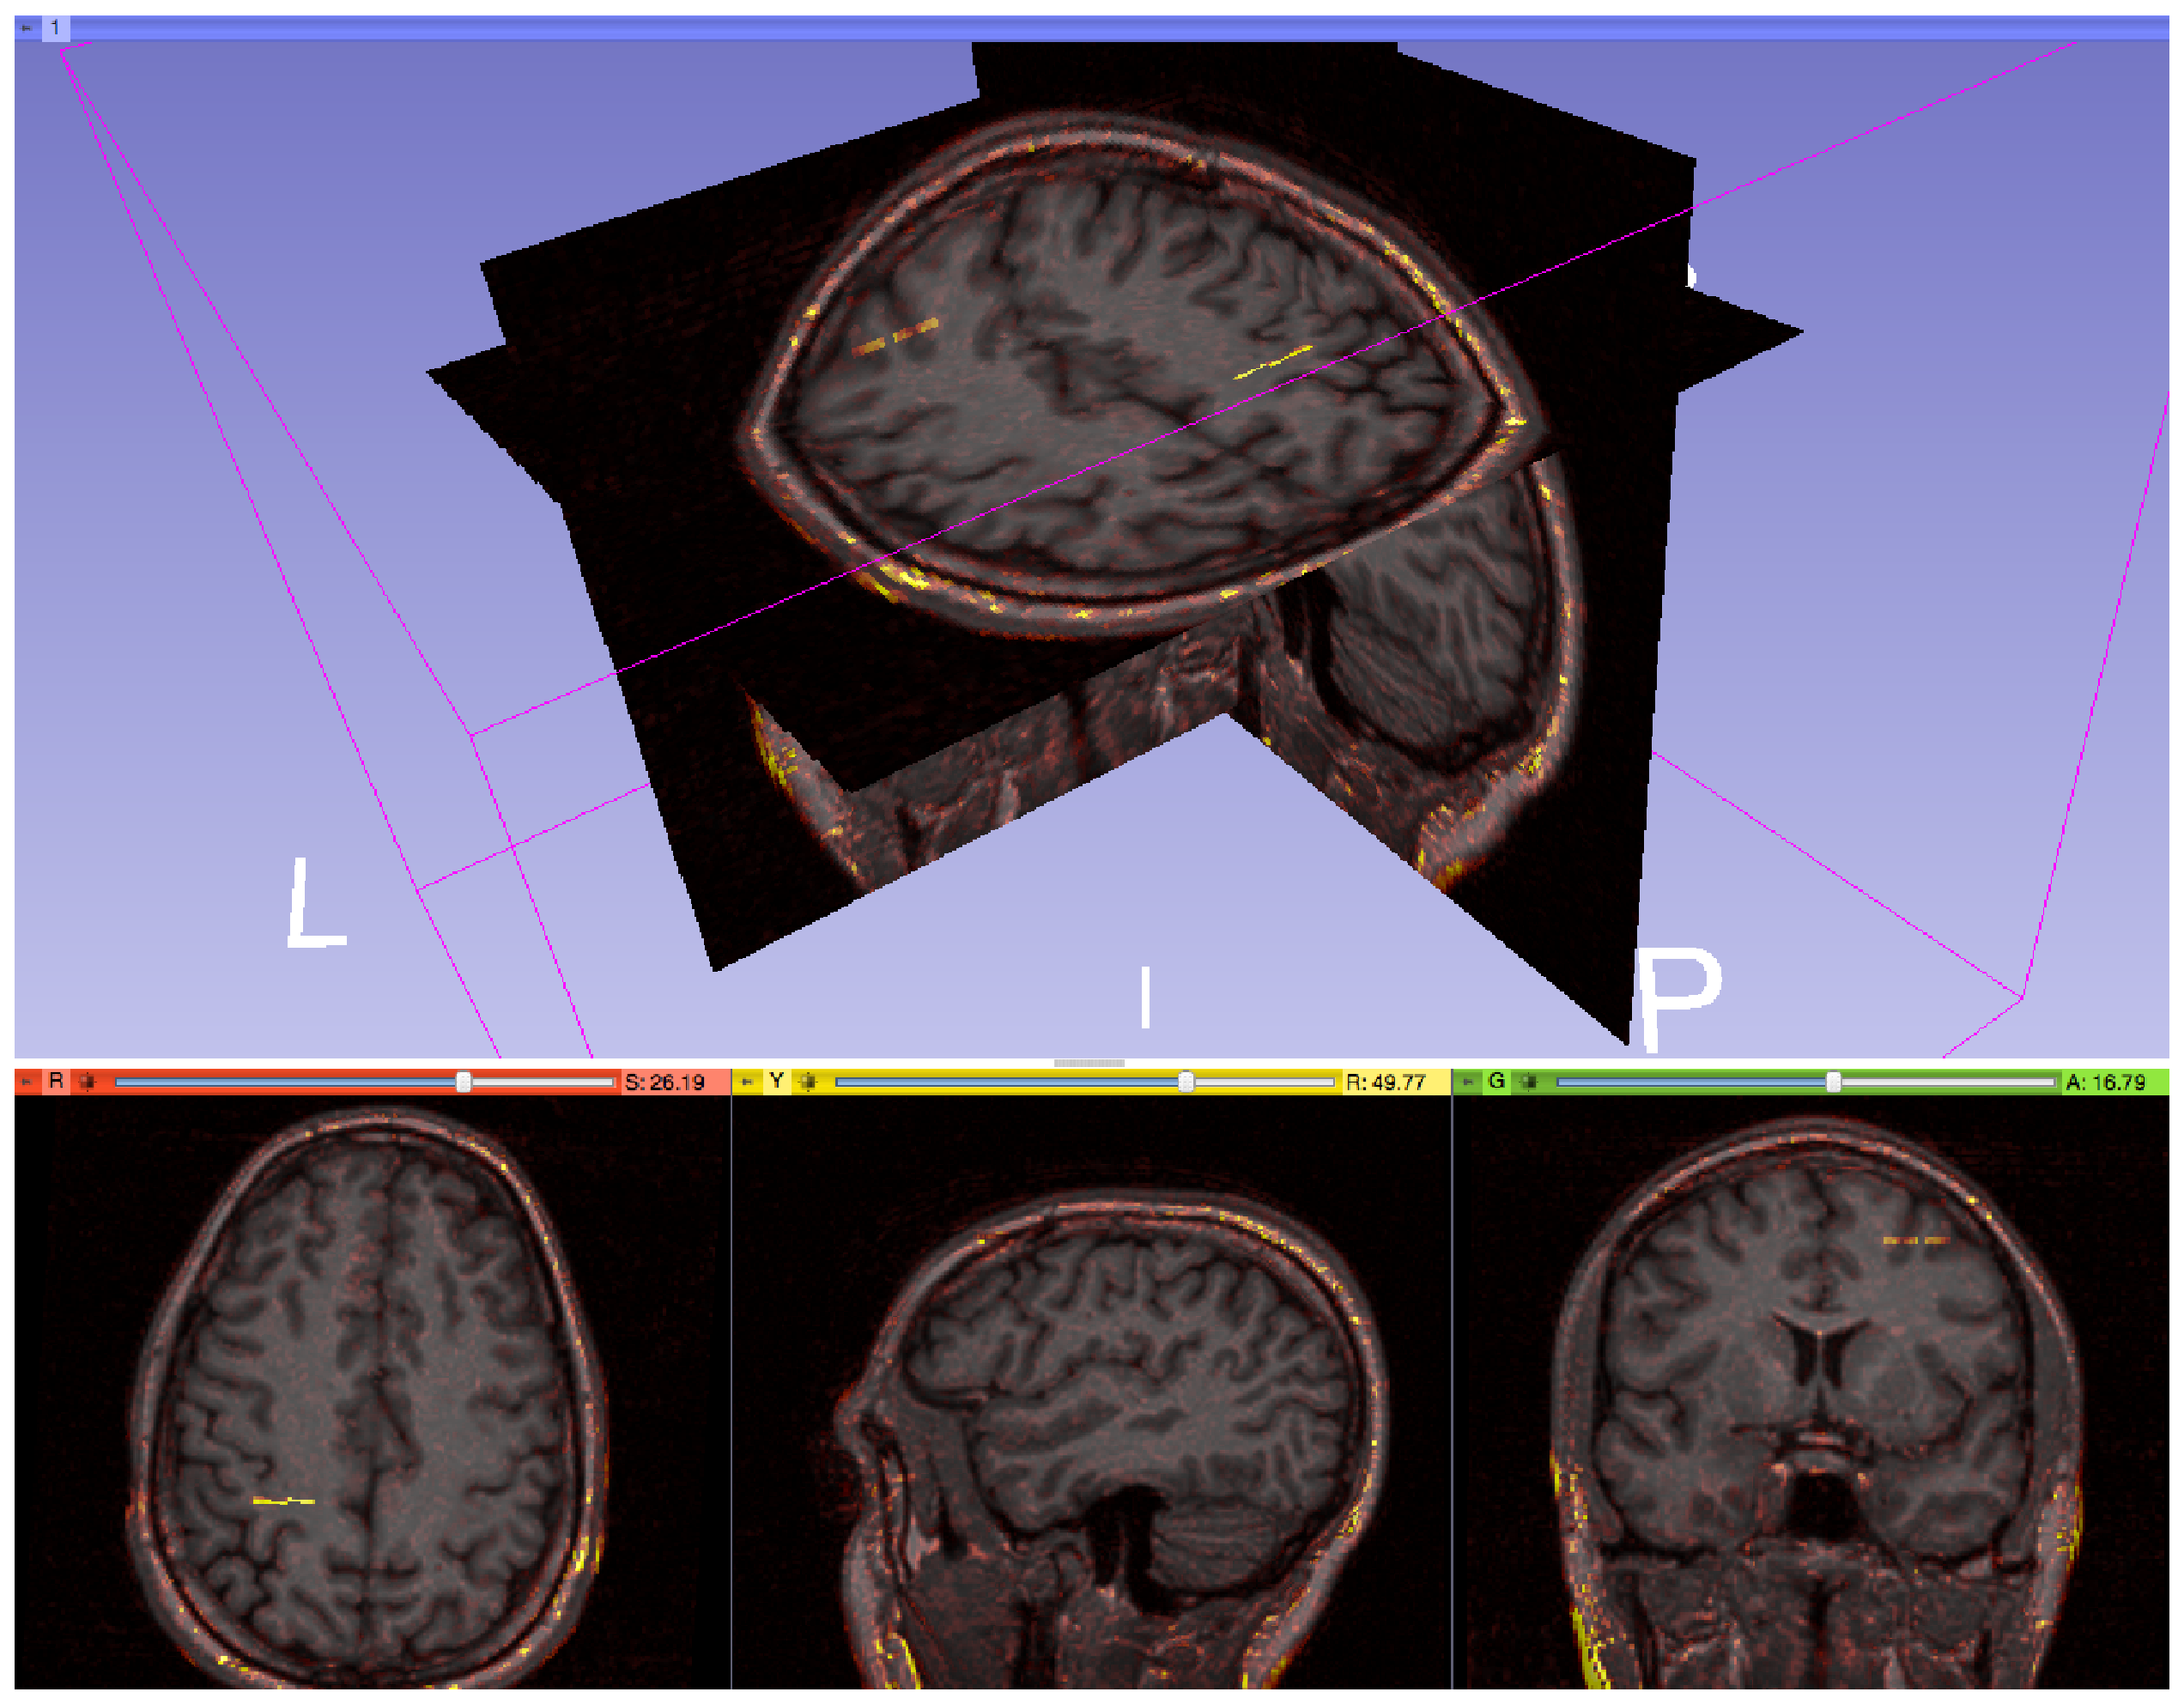
\includegraphics[scale=0.2]{/experiment_small/small_voxel1.eps}
  \caption{Artificial Small: Voxel-base method}
  \label{voxel_small1}
\end{figure}

Another angle of the result:

\begin{figure}[H]
  \centering
  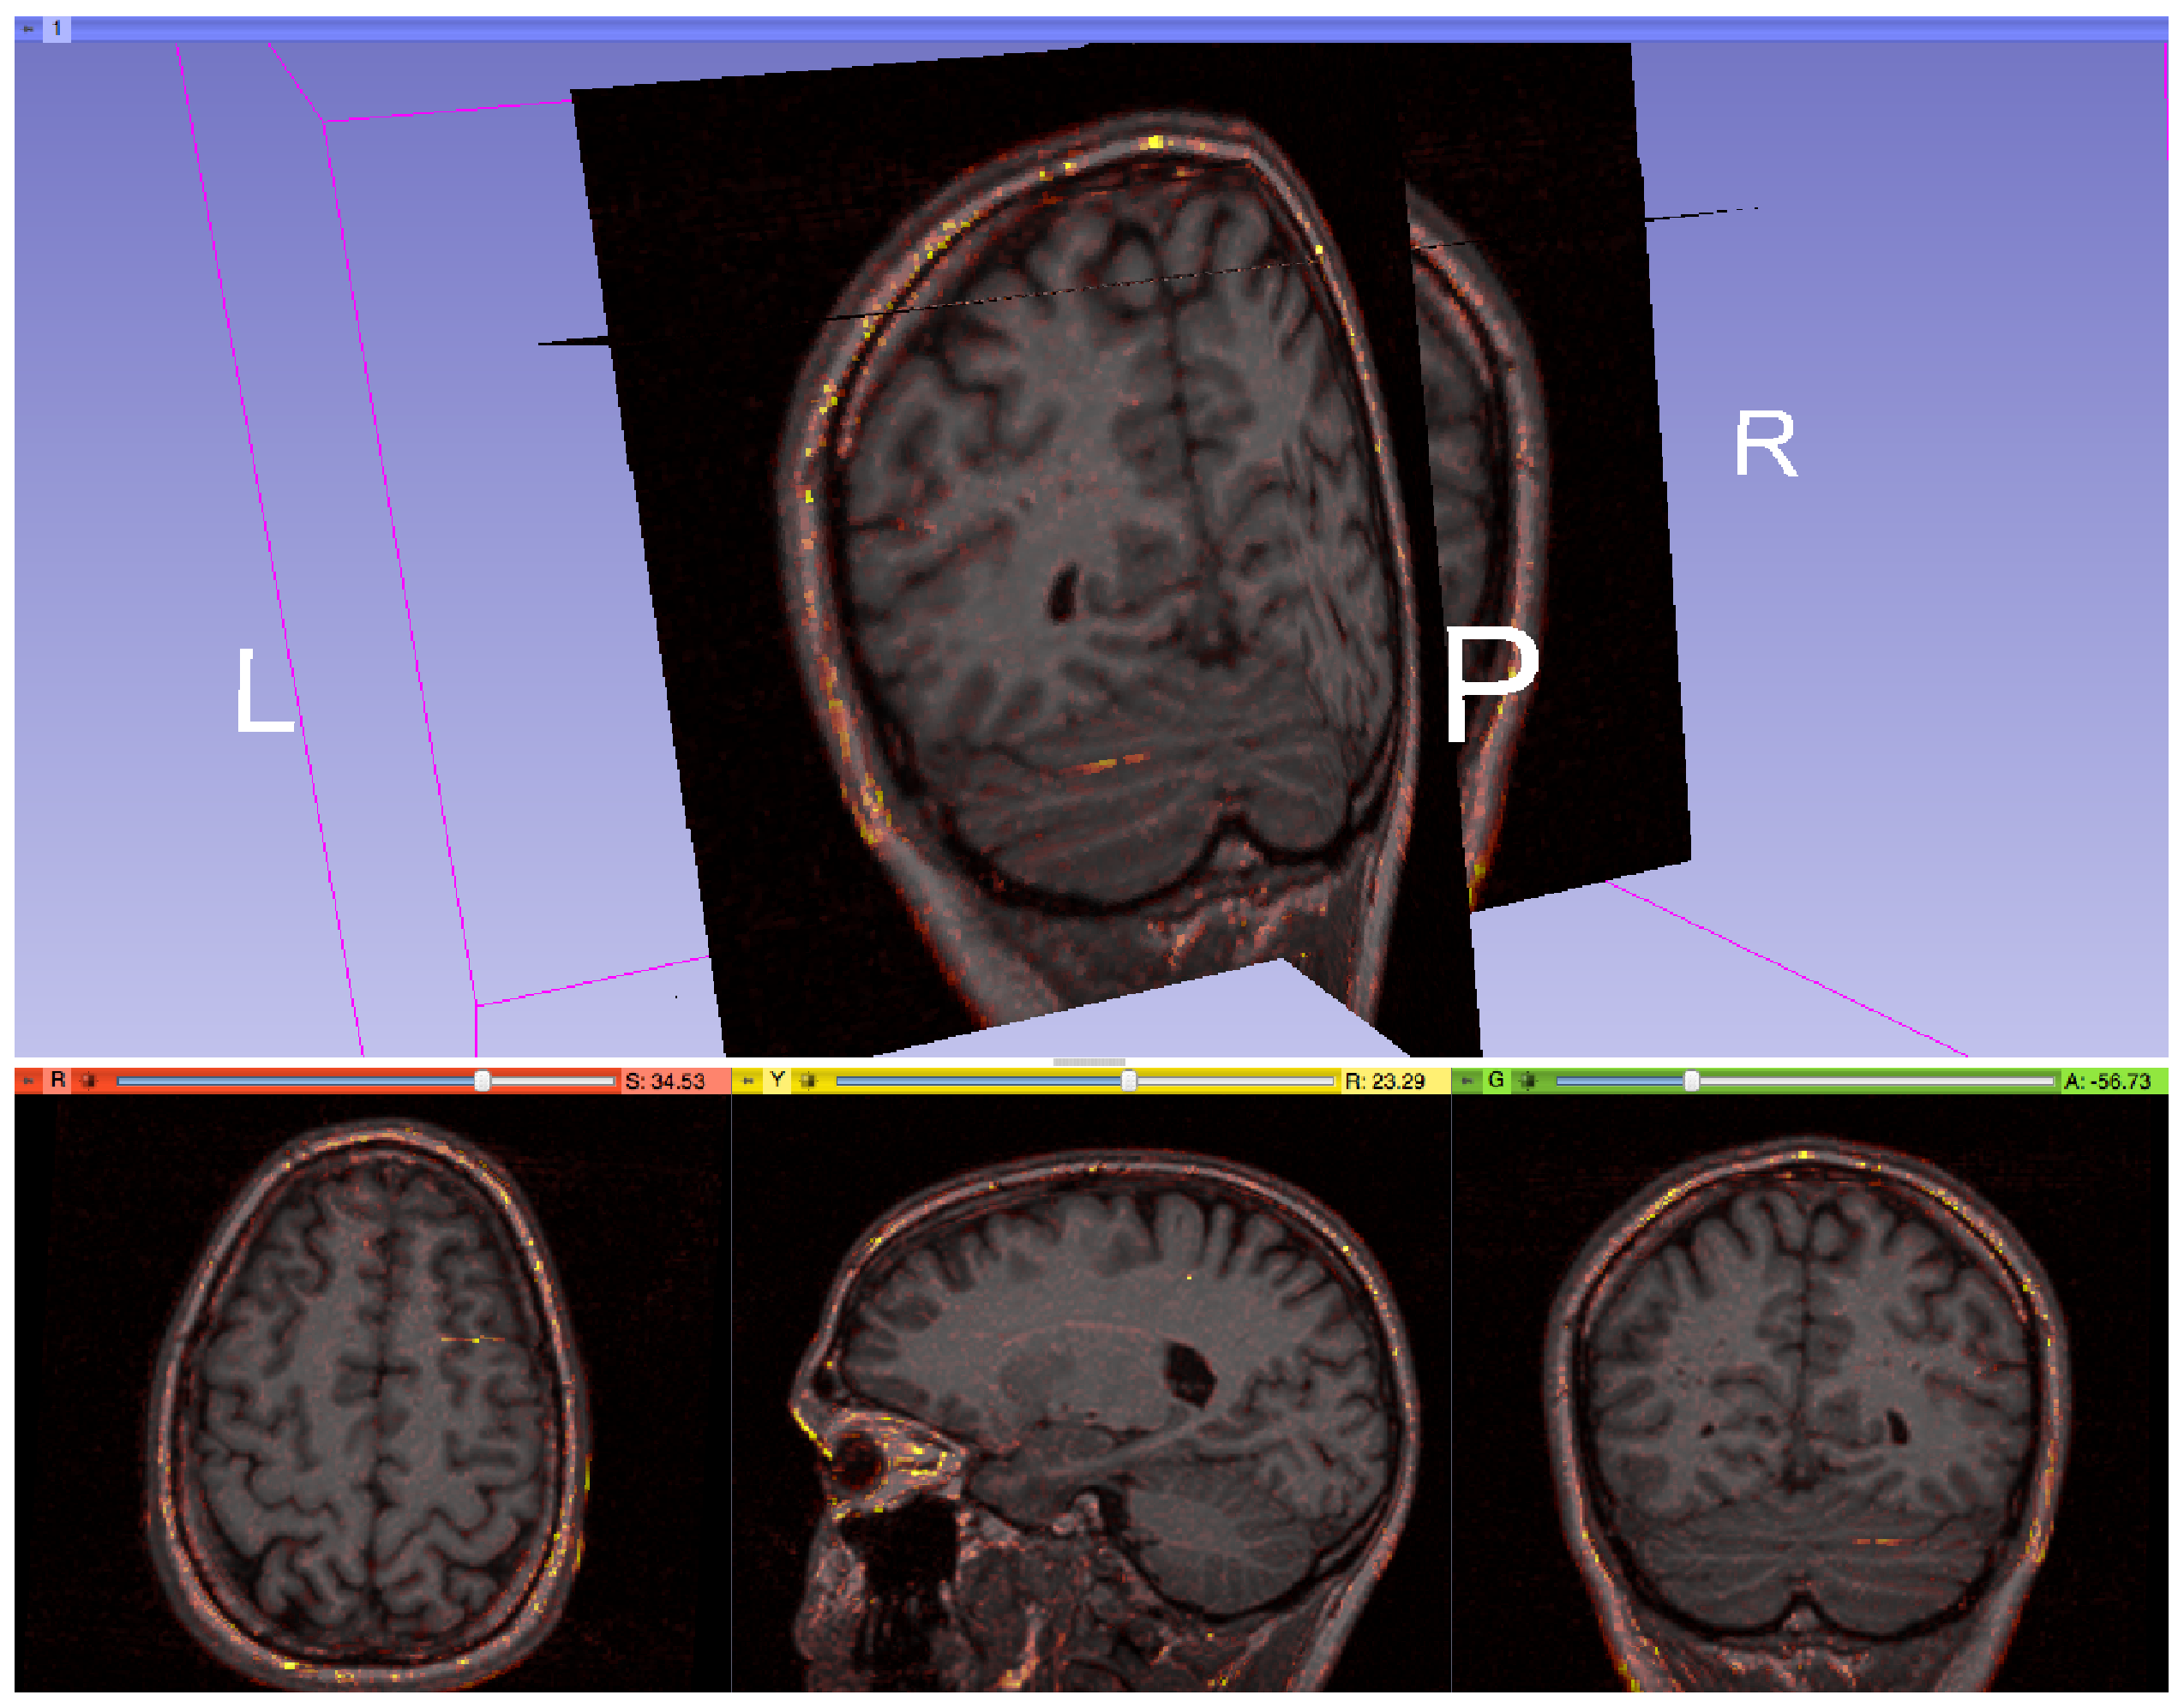
\includegraphics[scale=0.2]{/experiment_small/small_voxel2.eps}
  \caption{Artificial Small: Voxel-base method}
  \label{voxel_small2}
\end{figure}


\subsubsection{Tensor-based Method}
The result obtained is not very useful. It may be possible to find
some of the differences since we know their position in this
experiment. However, this would not be the case with real volumes as
it would be impossible to discern between real differences and those
produced by imperfections in the method.

The parameters used to obtain this result are:
\begin{description}
\item \textit{Deformation field smoothing sigma:} 3.5
\item \textit{Shrinkage percentage:} 70
\item \textit{Growth percentage:} 80
\end{description}

Note that in this case the parameter for deformation field smoothing
sigma is higher. This produced a smoother deformation field after the
registration, which improved the results to some extent; even though
the final result is still not good enough.

\begin{figure}[H]
  \centering
  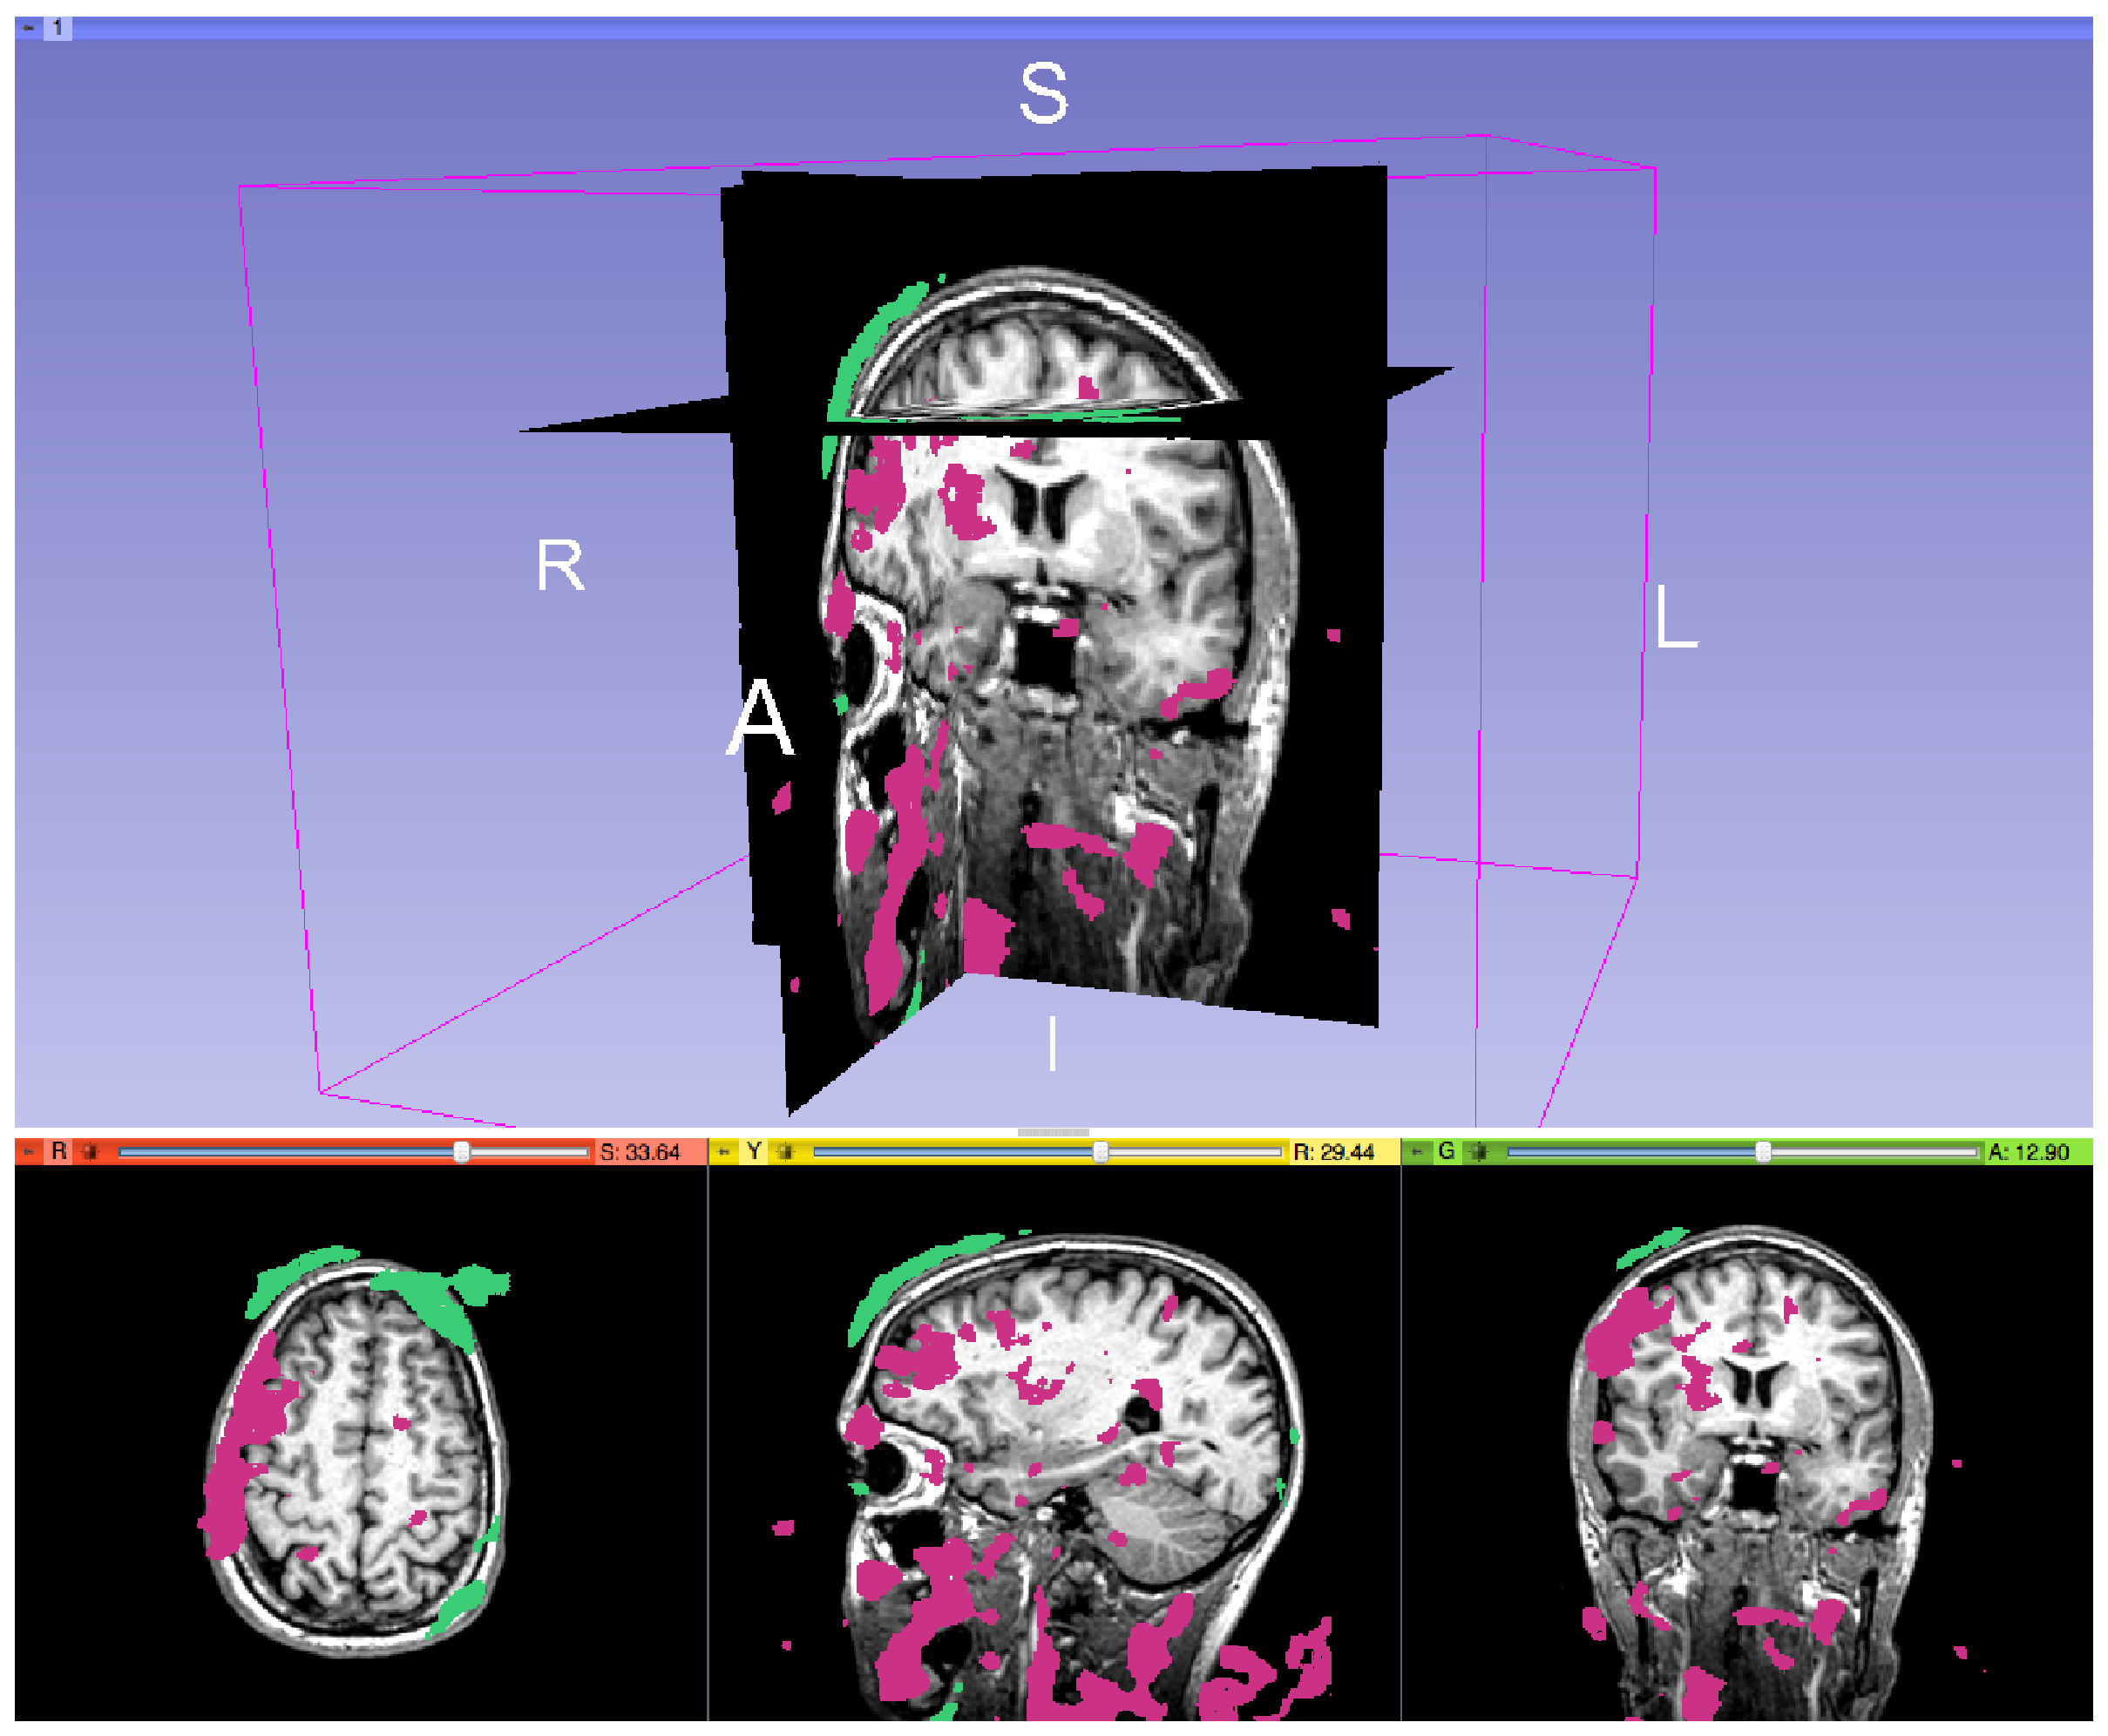
\includegraphics[scale=0.2]{/experiment_small/tensor_70-80_small1.eps}
  \caption{Artificial Small: Tensor-base method}
  \label{tensor_small1}
\end{figure}

Another angle of the result:

\begin{figure}[H]
  \centering
  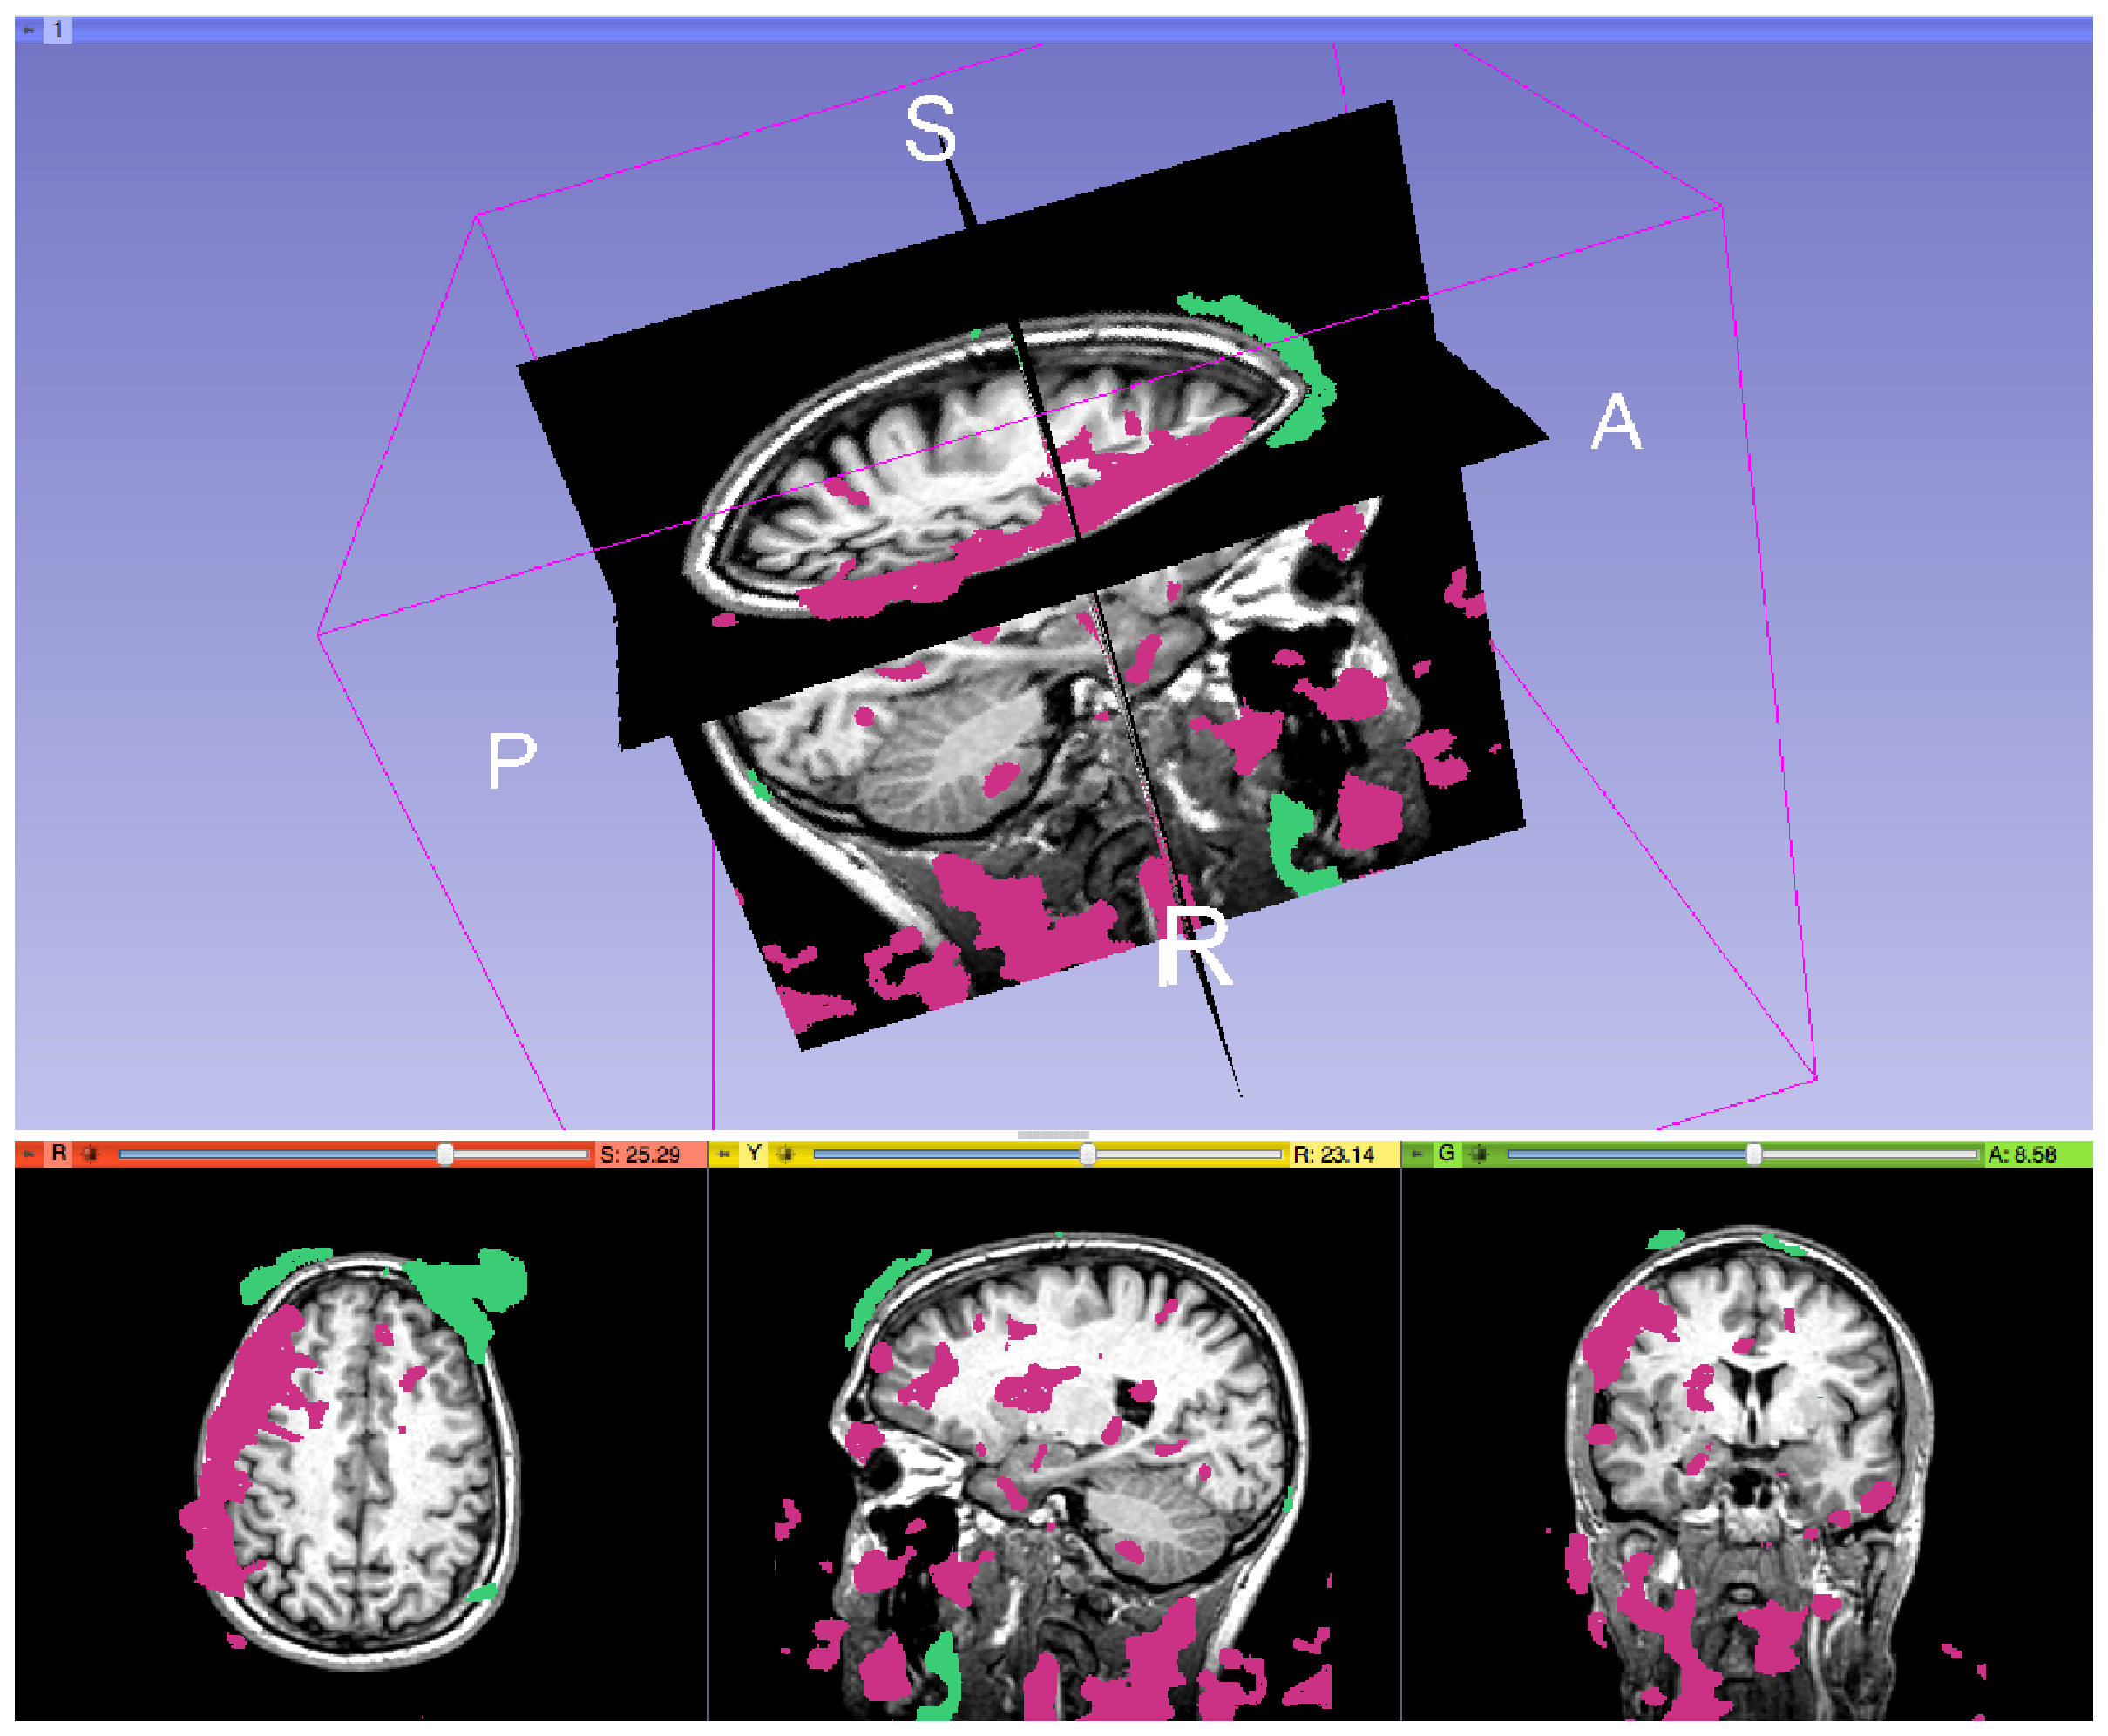
\includegraphics[scale=0.2]{/experiment_small/tensor_70-80_small2.eps}
  \caption{Artificial Small: Tensor-base method}
  \label{tensor_small2}
\end{figure}

\section{Real Differences Results}

\subsection{Patient 1}
This patient presents small differences in the parietal lobe, the
differences can be seen as red lines in the voxel-based method's result
and pink or green areas in the tensor-based method's result.

\subsubsection{Voxel-based Method}
The registration method used was \textit{Affine registration}.

\begin{figure}[H]
  \centering
  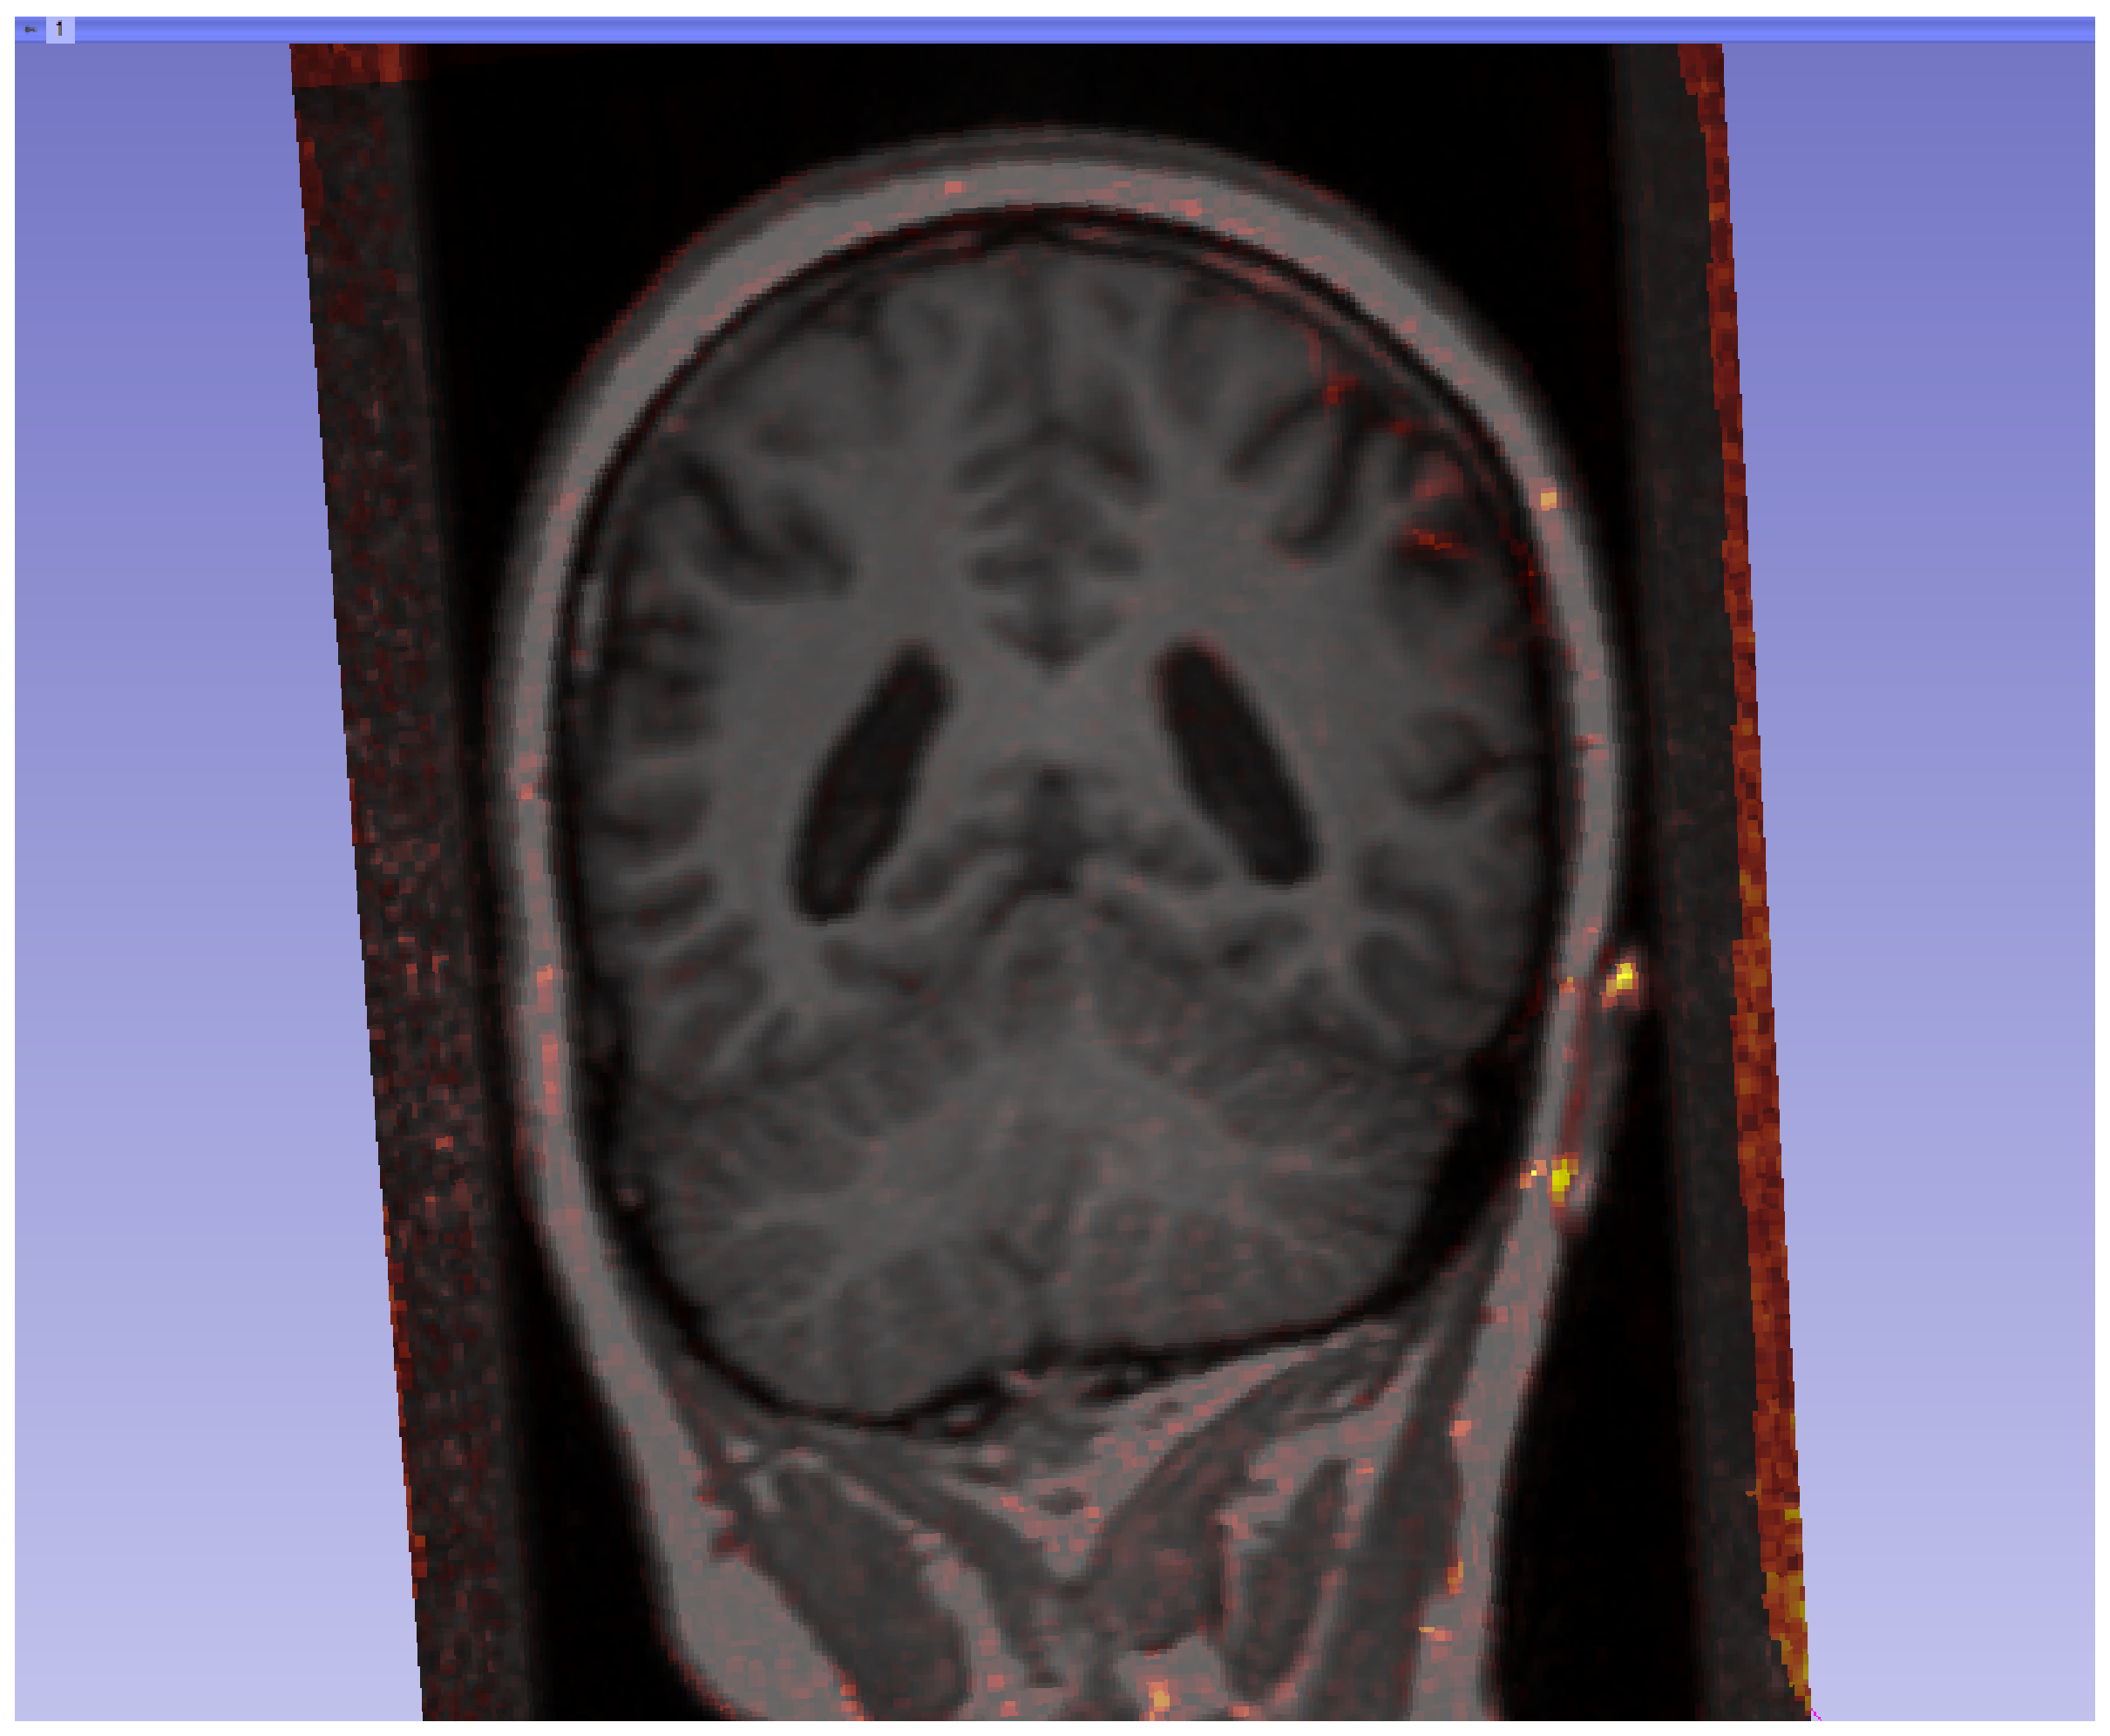
\includegraphics[scale=0.2]{/experiment_CL_P1/CL_Coronal.eps}
  \caption{Voxel-based method. Patient 1: Coronal plane}
  \label{CL_Coronal}
\end{figure}

\begin{figure}[H]
  \centering
  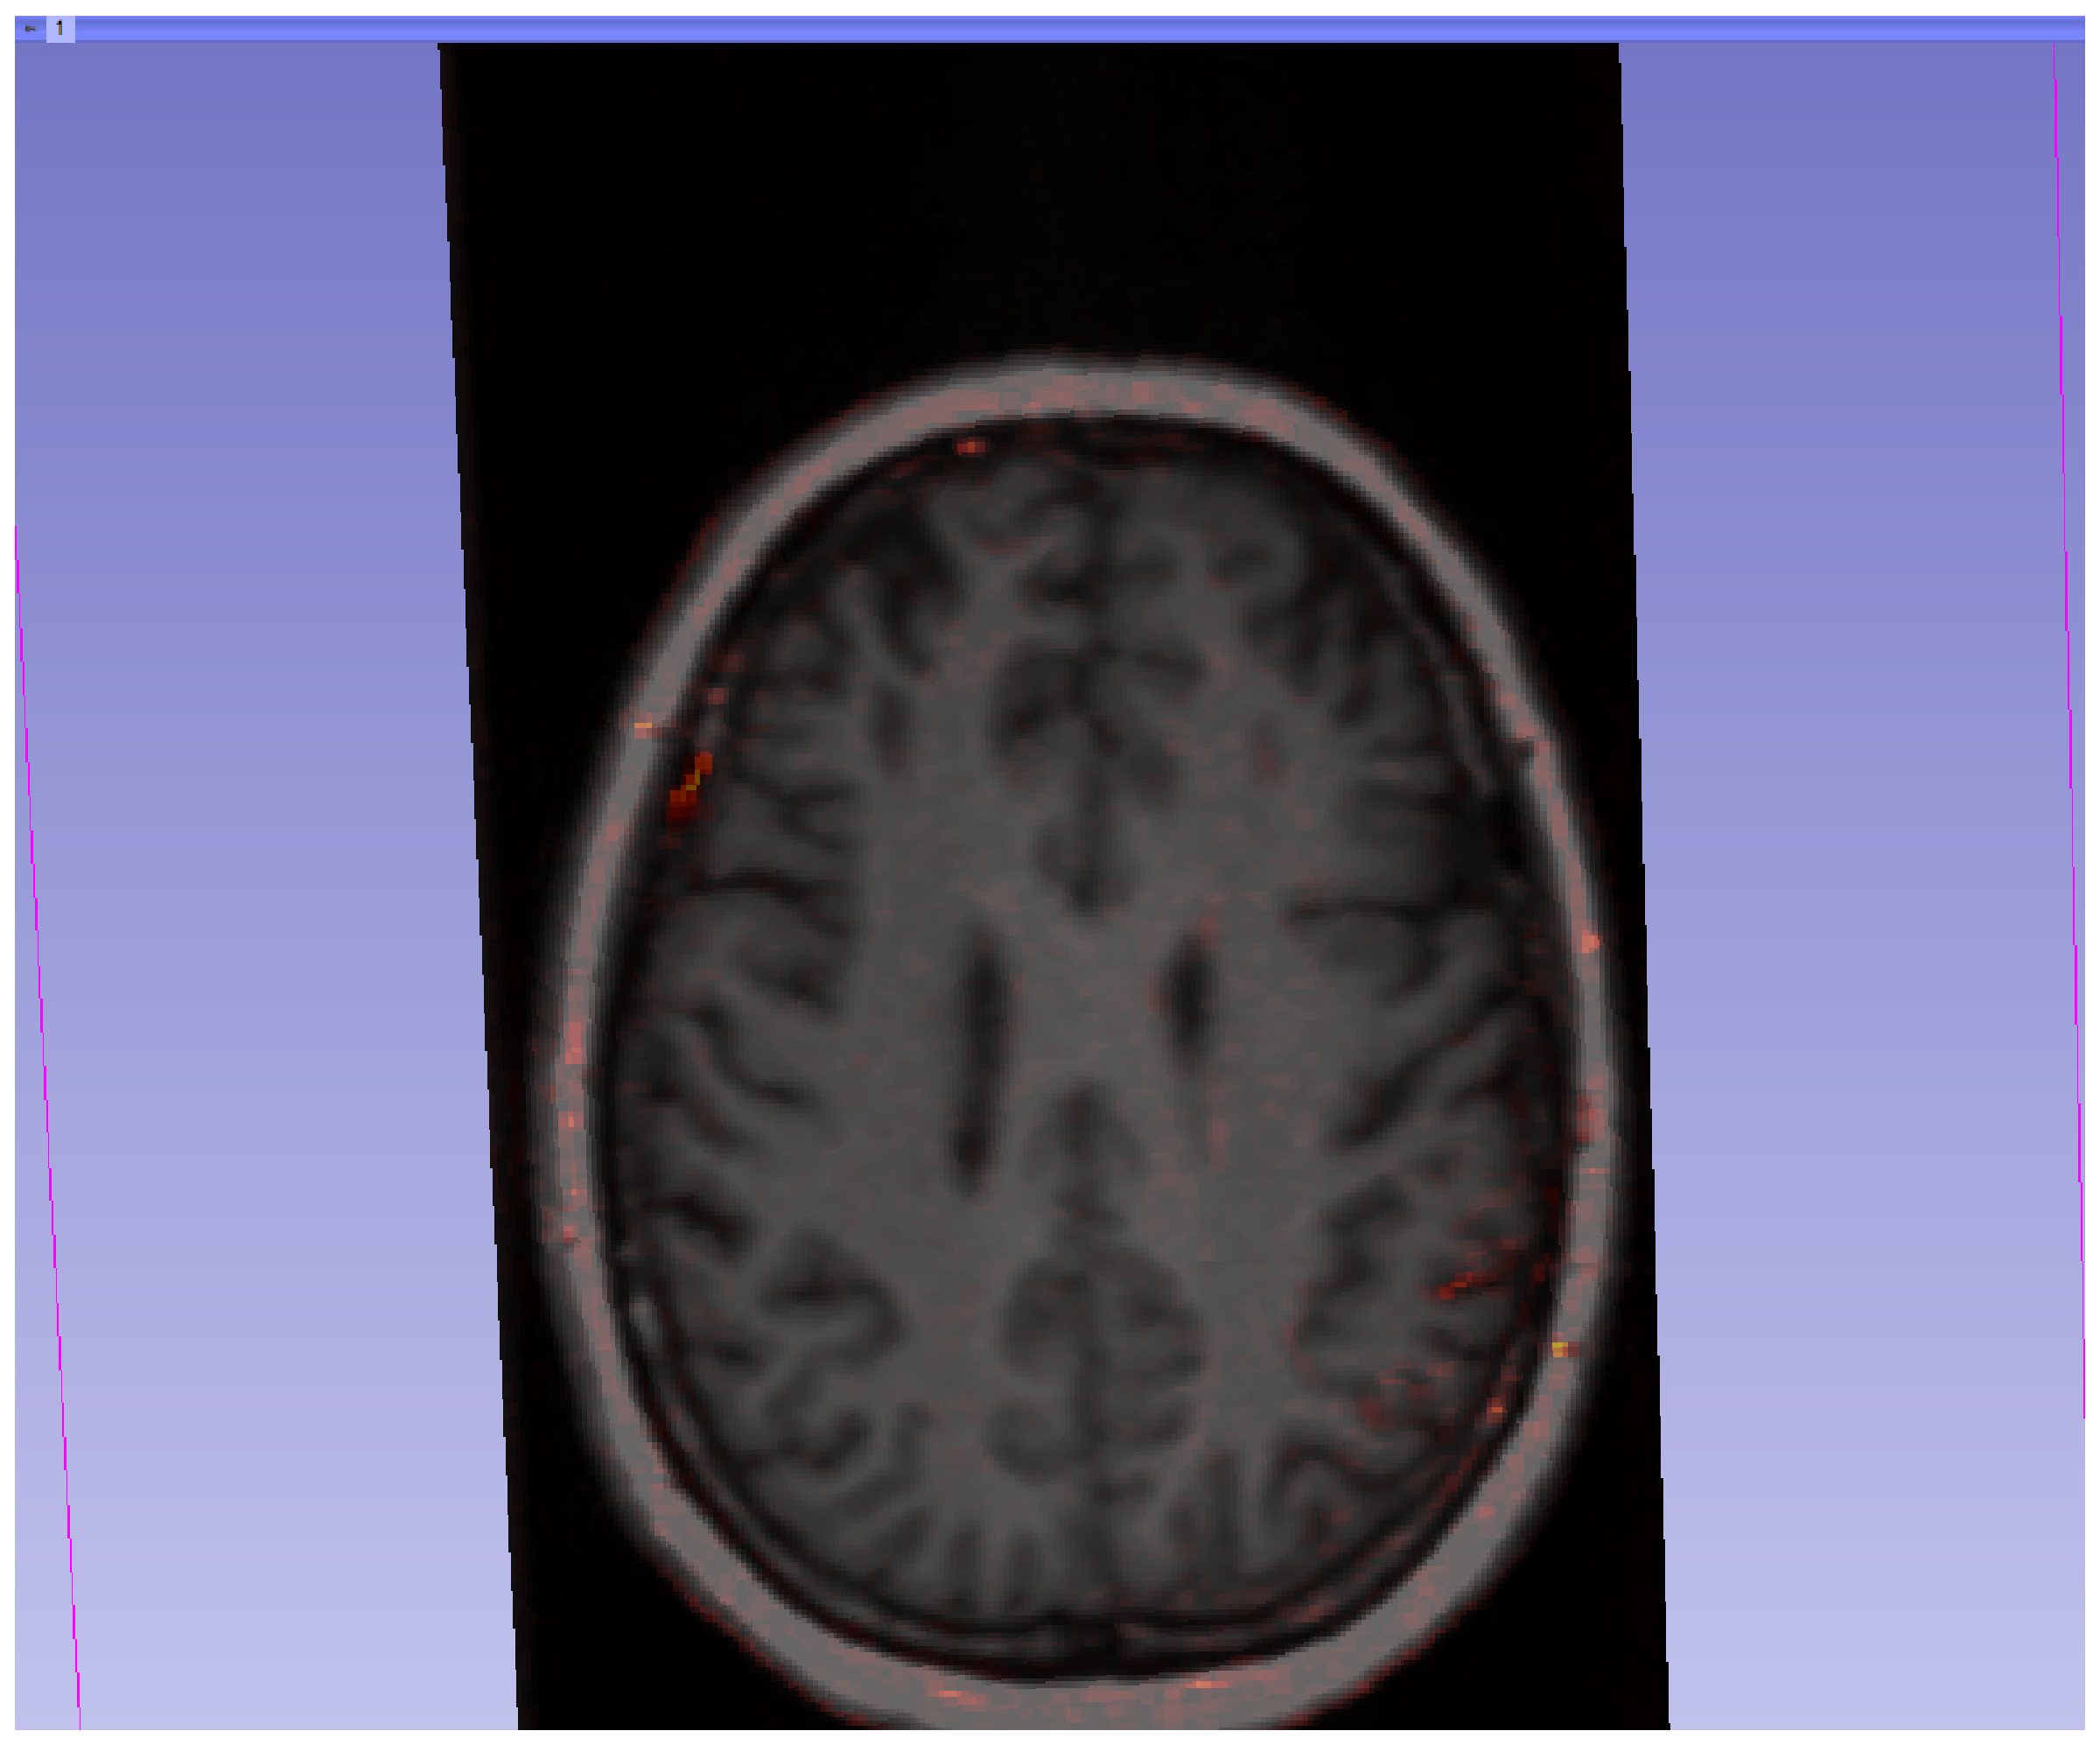
\includegraphics[scale=0.2]{/experiment_CL_P1/CL_Traversal.eps}
  \caption{Voxel-based method. Patient 1: Traversal plane}
  \label{CL_Traversal}
\end{figure}

\begin{figure}[H]
  \centering
  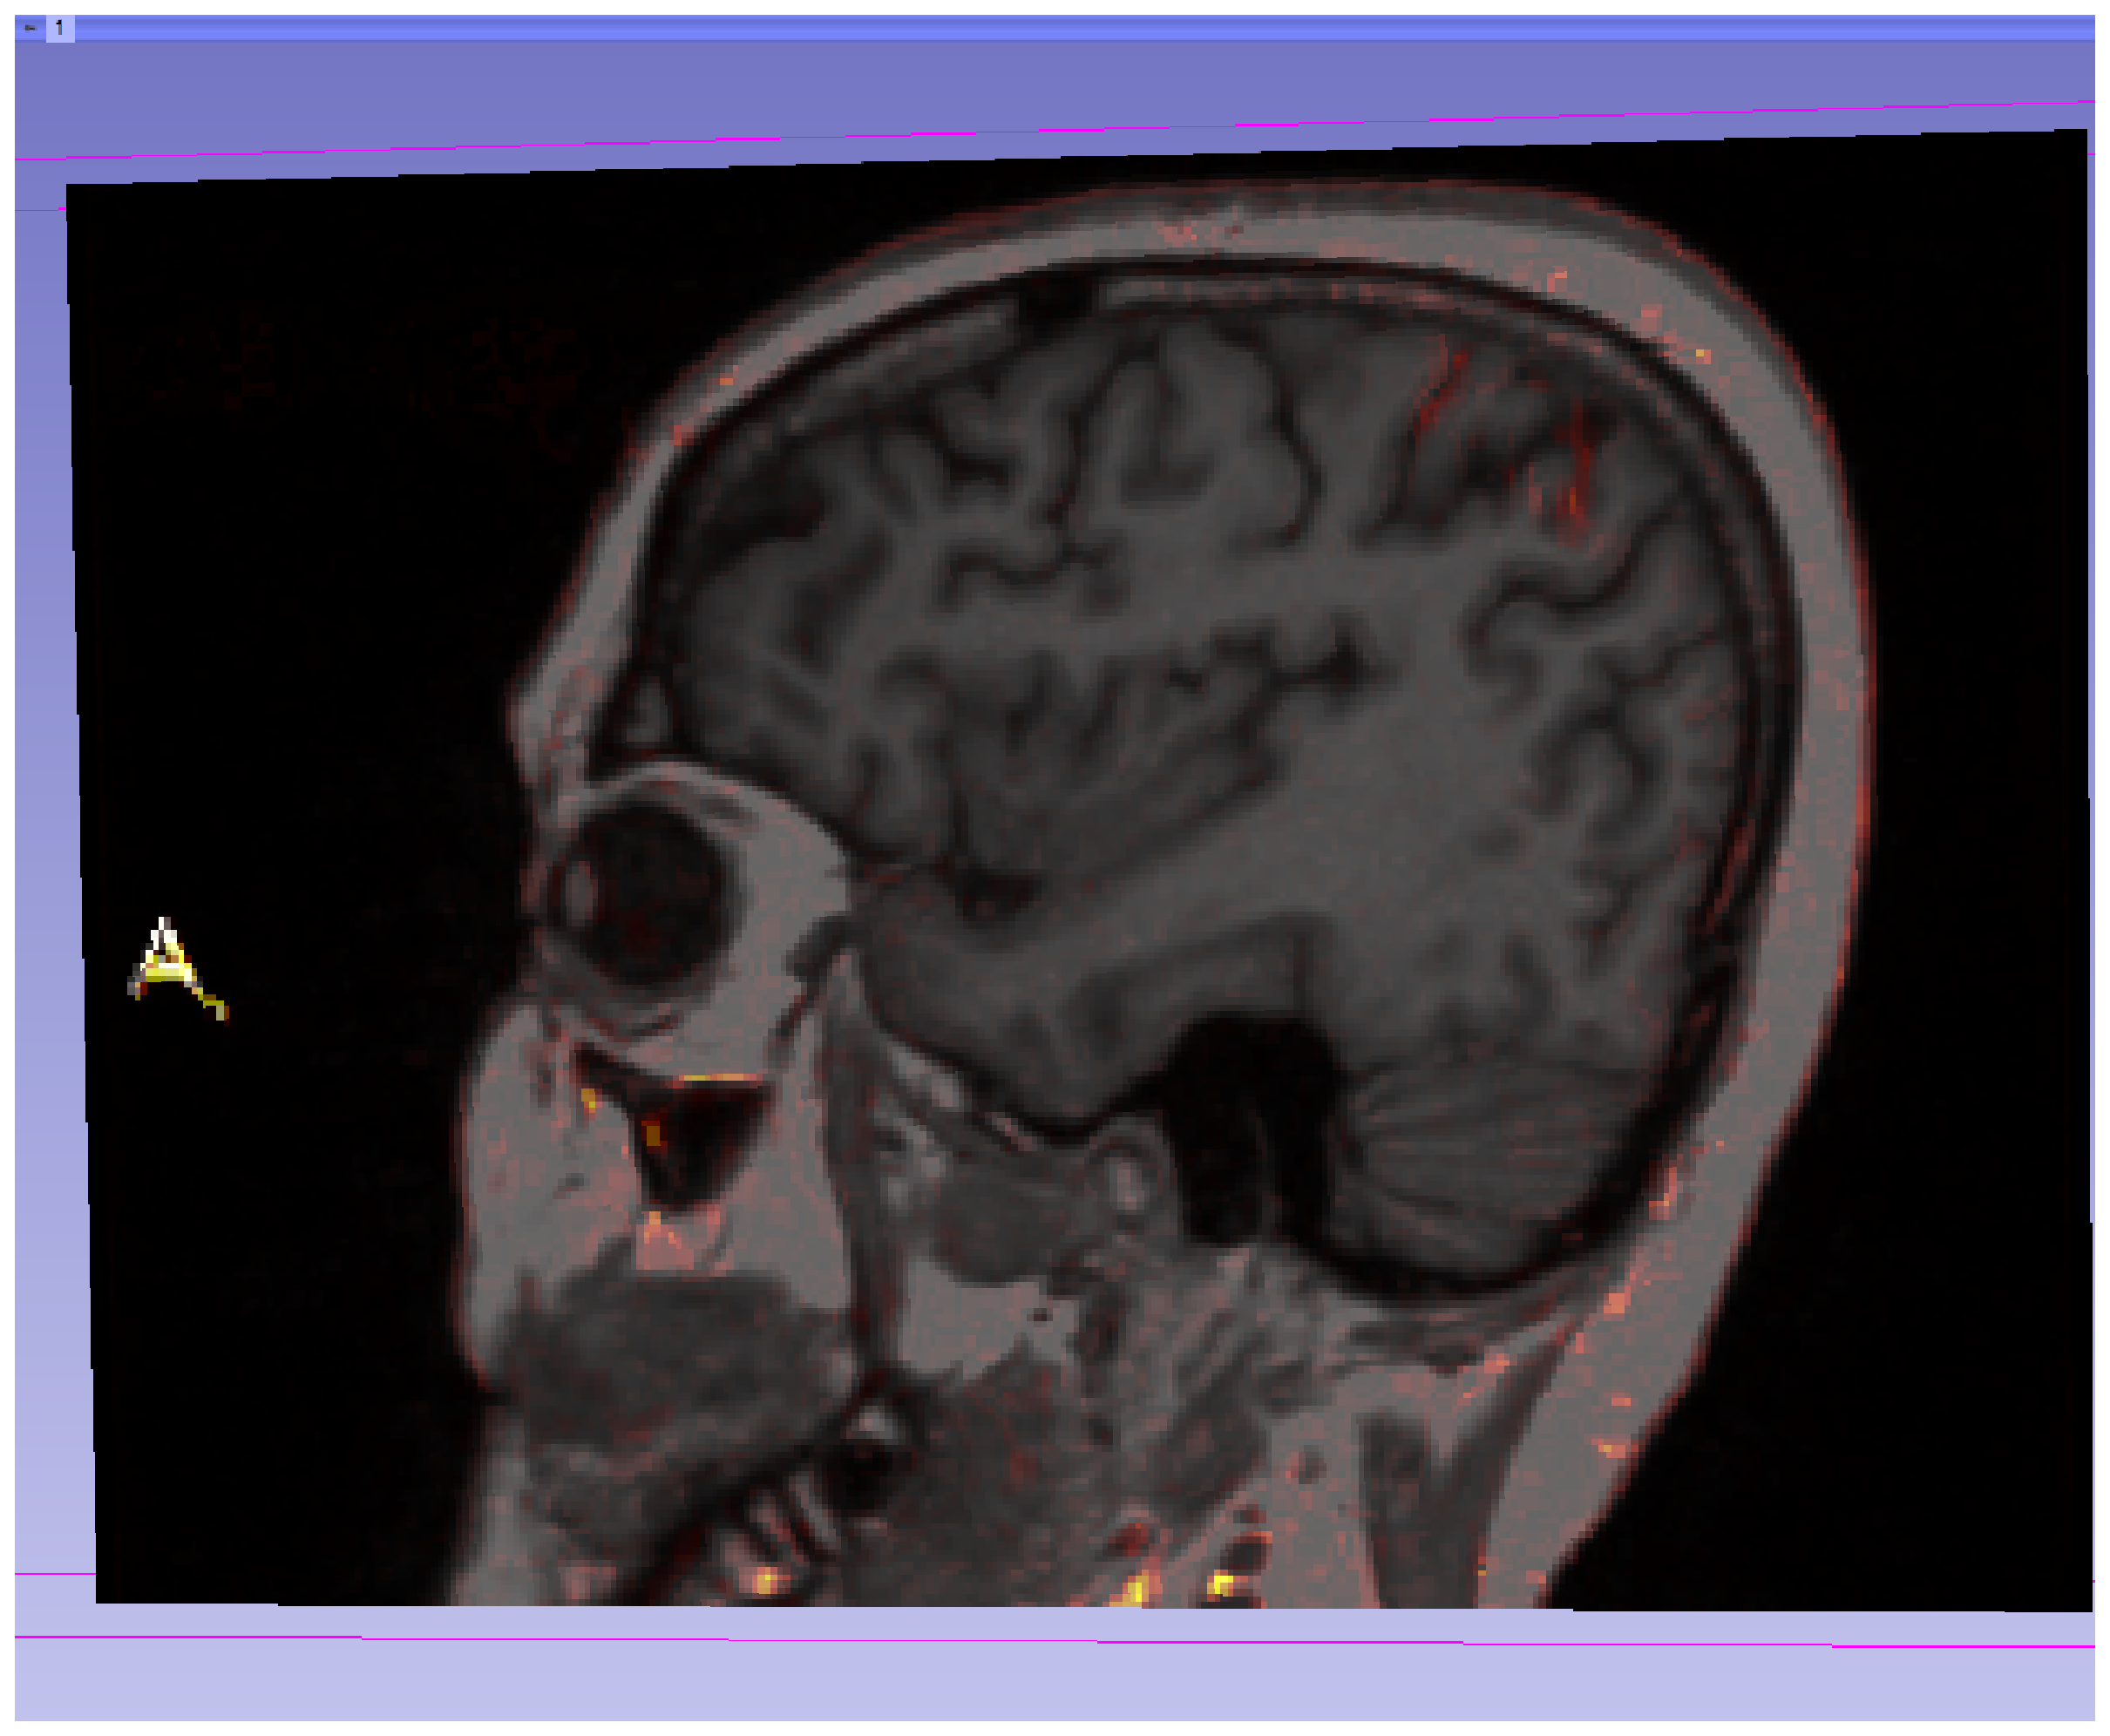
\includegraphics[scale=0.2]{/experiment_CL_P1/CL_Sagittal.eps}
  \caption{Voxel-based method. Patient 1: Sagittal plane}
  \label{CL_Sagittal}
\end{figure}


\subsubsection{Tensor-based Method}
Parameters used:
\begin{description}
\item \textit{Deformation field smoothing sigma:} 2.5
\item \textit{Shrinkage percentage:} 70
\item \textit{Growth percentage:} 75
\end{description}

\begin{figure}[H]
  \centering
  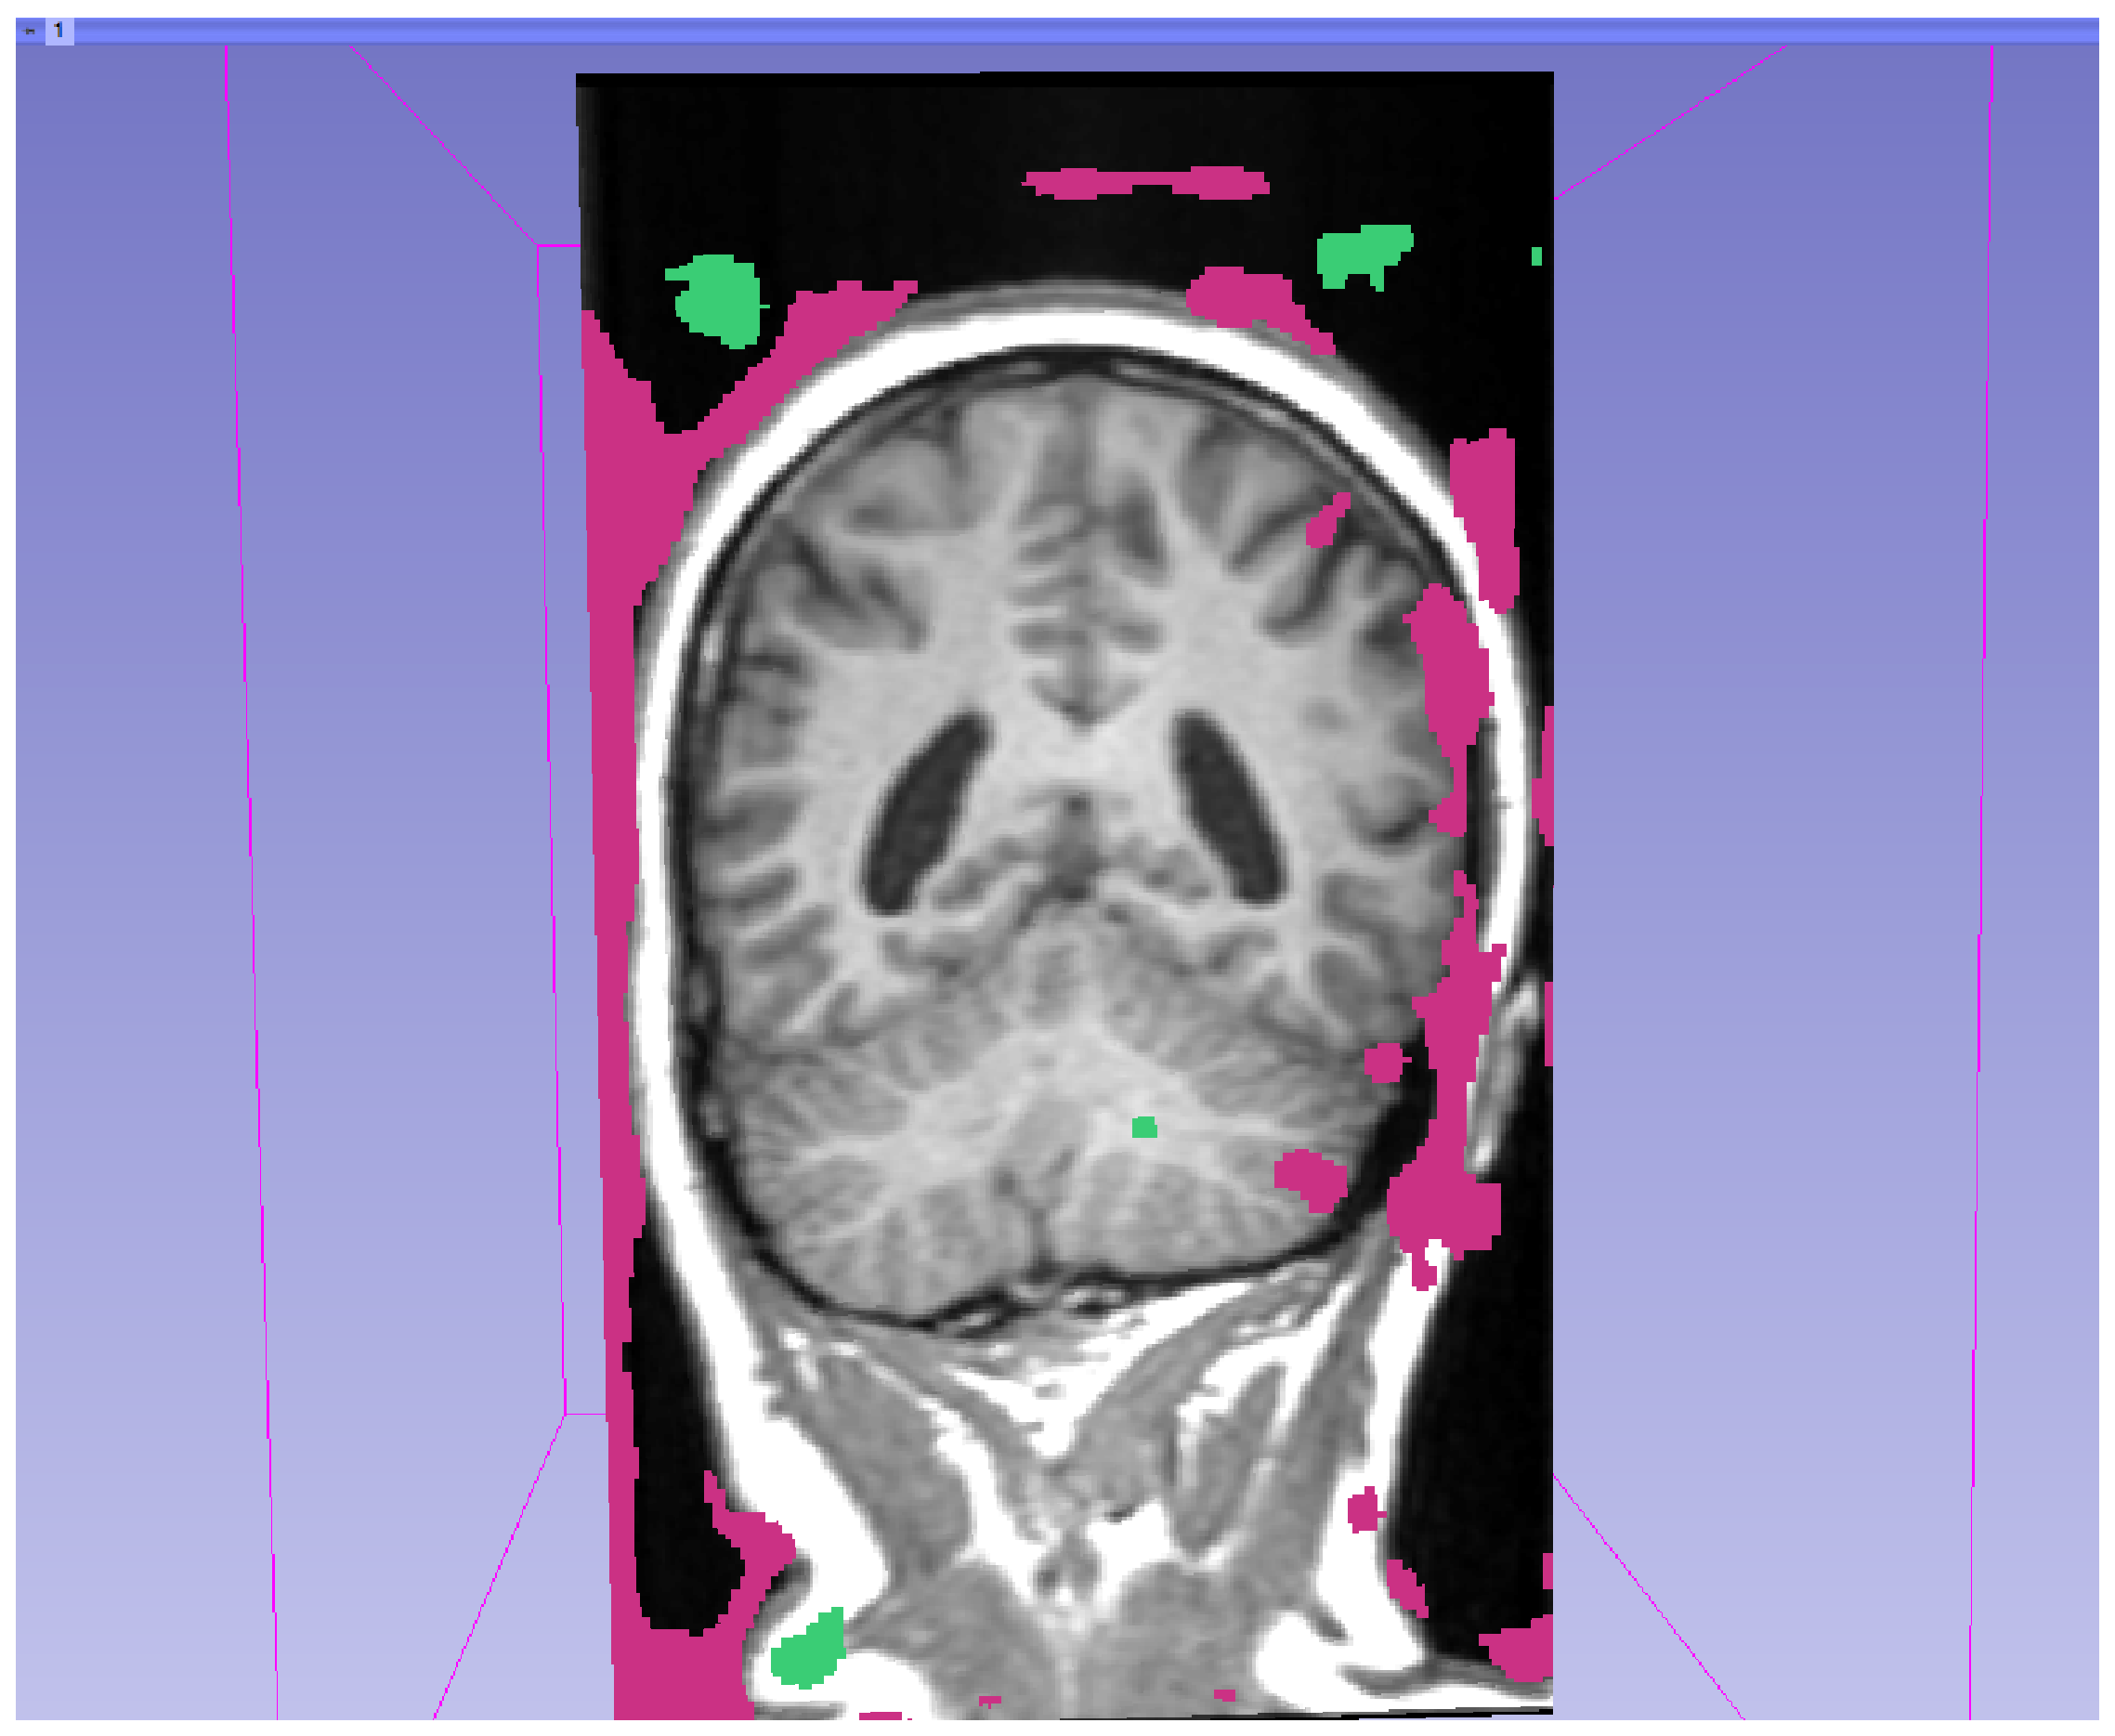
\includegraphics[scale=0.2]{/experiment_CL_P1/CL_Tensor_Coronal.eps}
  \caption{Tensor-based method. Patient 1: Coronal plane}
  \label{CL_TCoronal}
\end{figure}

\begin{figure}[H]
  \centering
  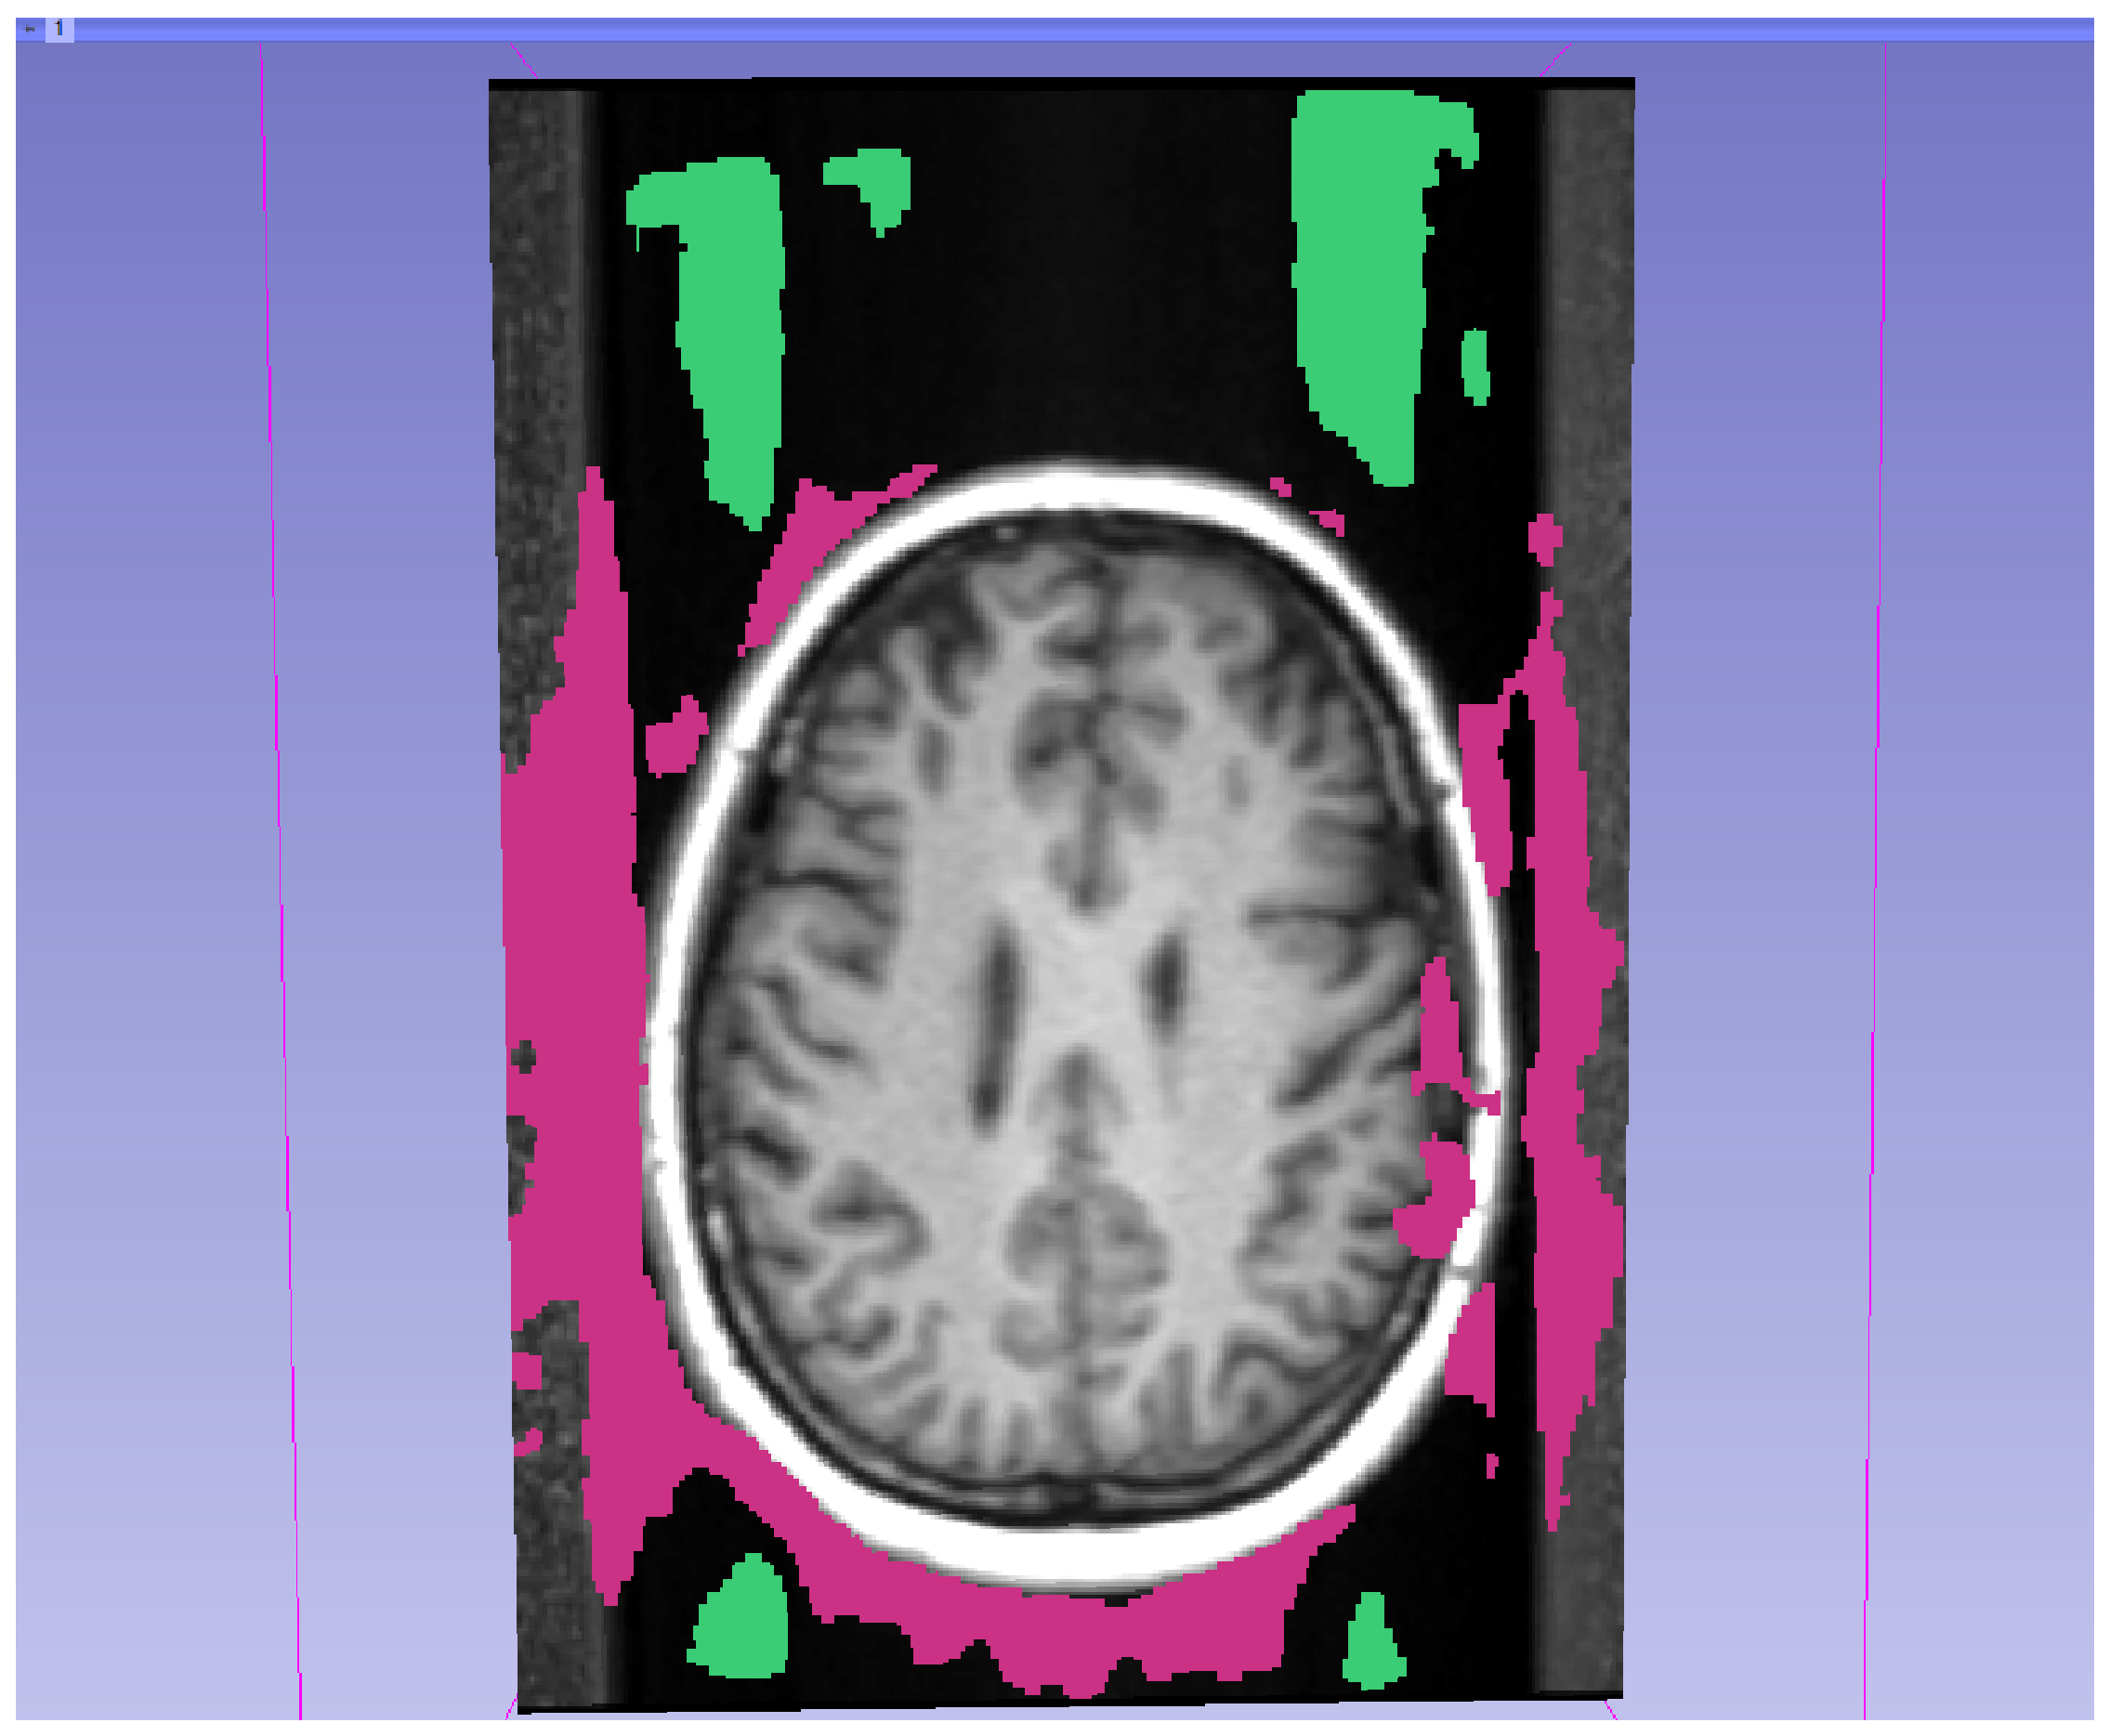
\includegraphics[scale=0.2]{/experiment_CL_P1/CL_Tensor_Traversal.eps}
  \caption{Tensor-based method. Patient 1: Traversal plane}
  \label{CL_TTraversal}
\end{figure}

\begin{figure}[H]
  \centering
  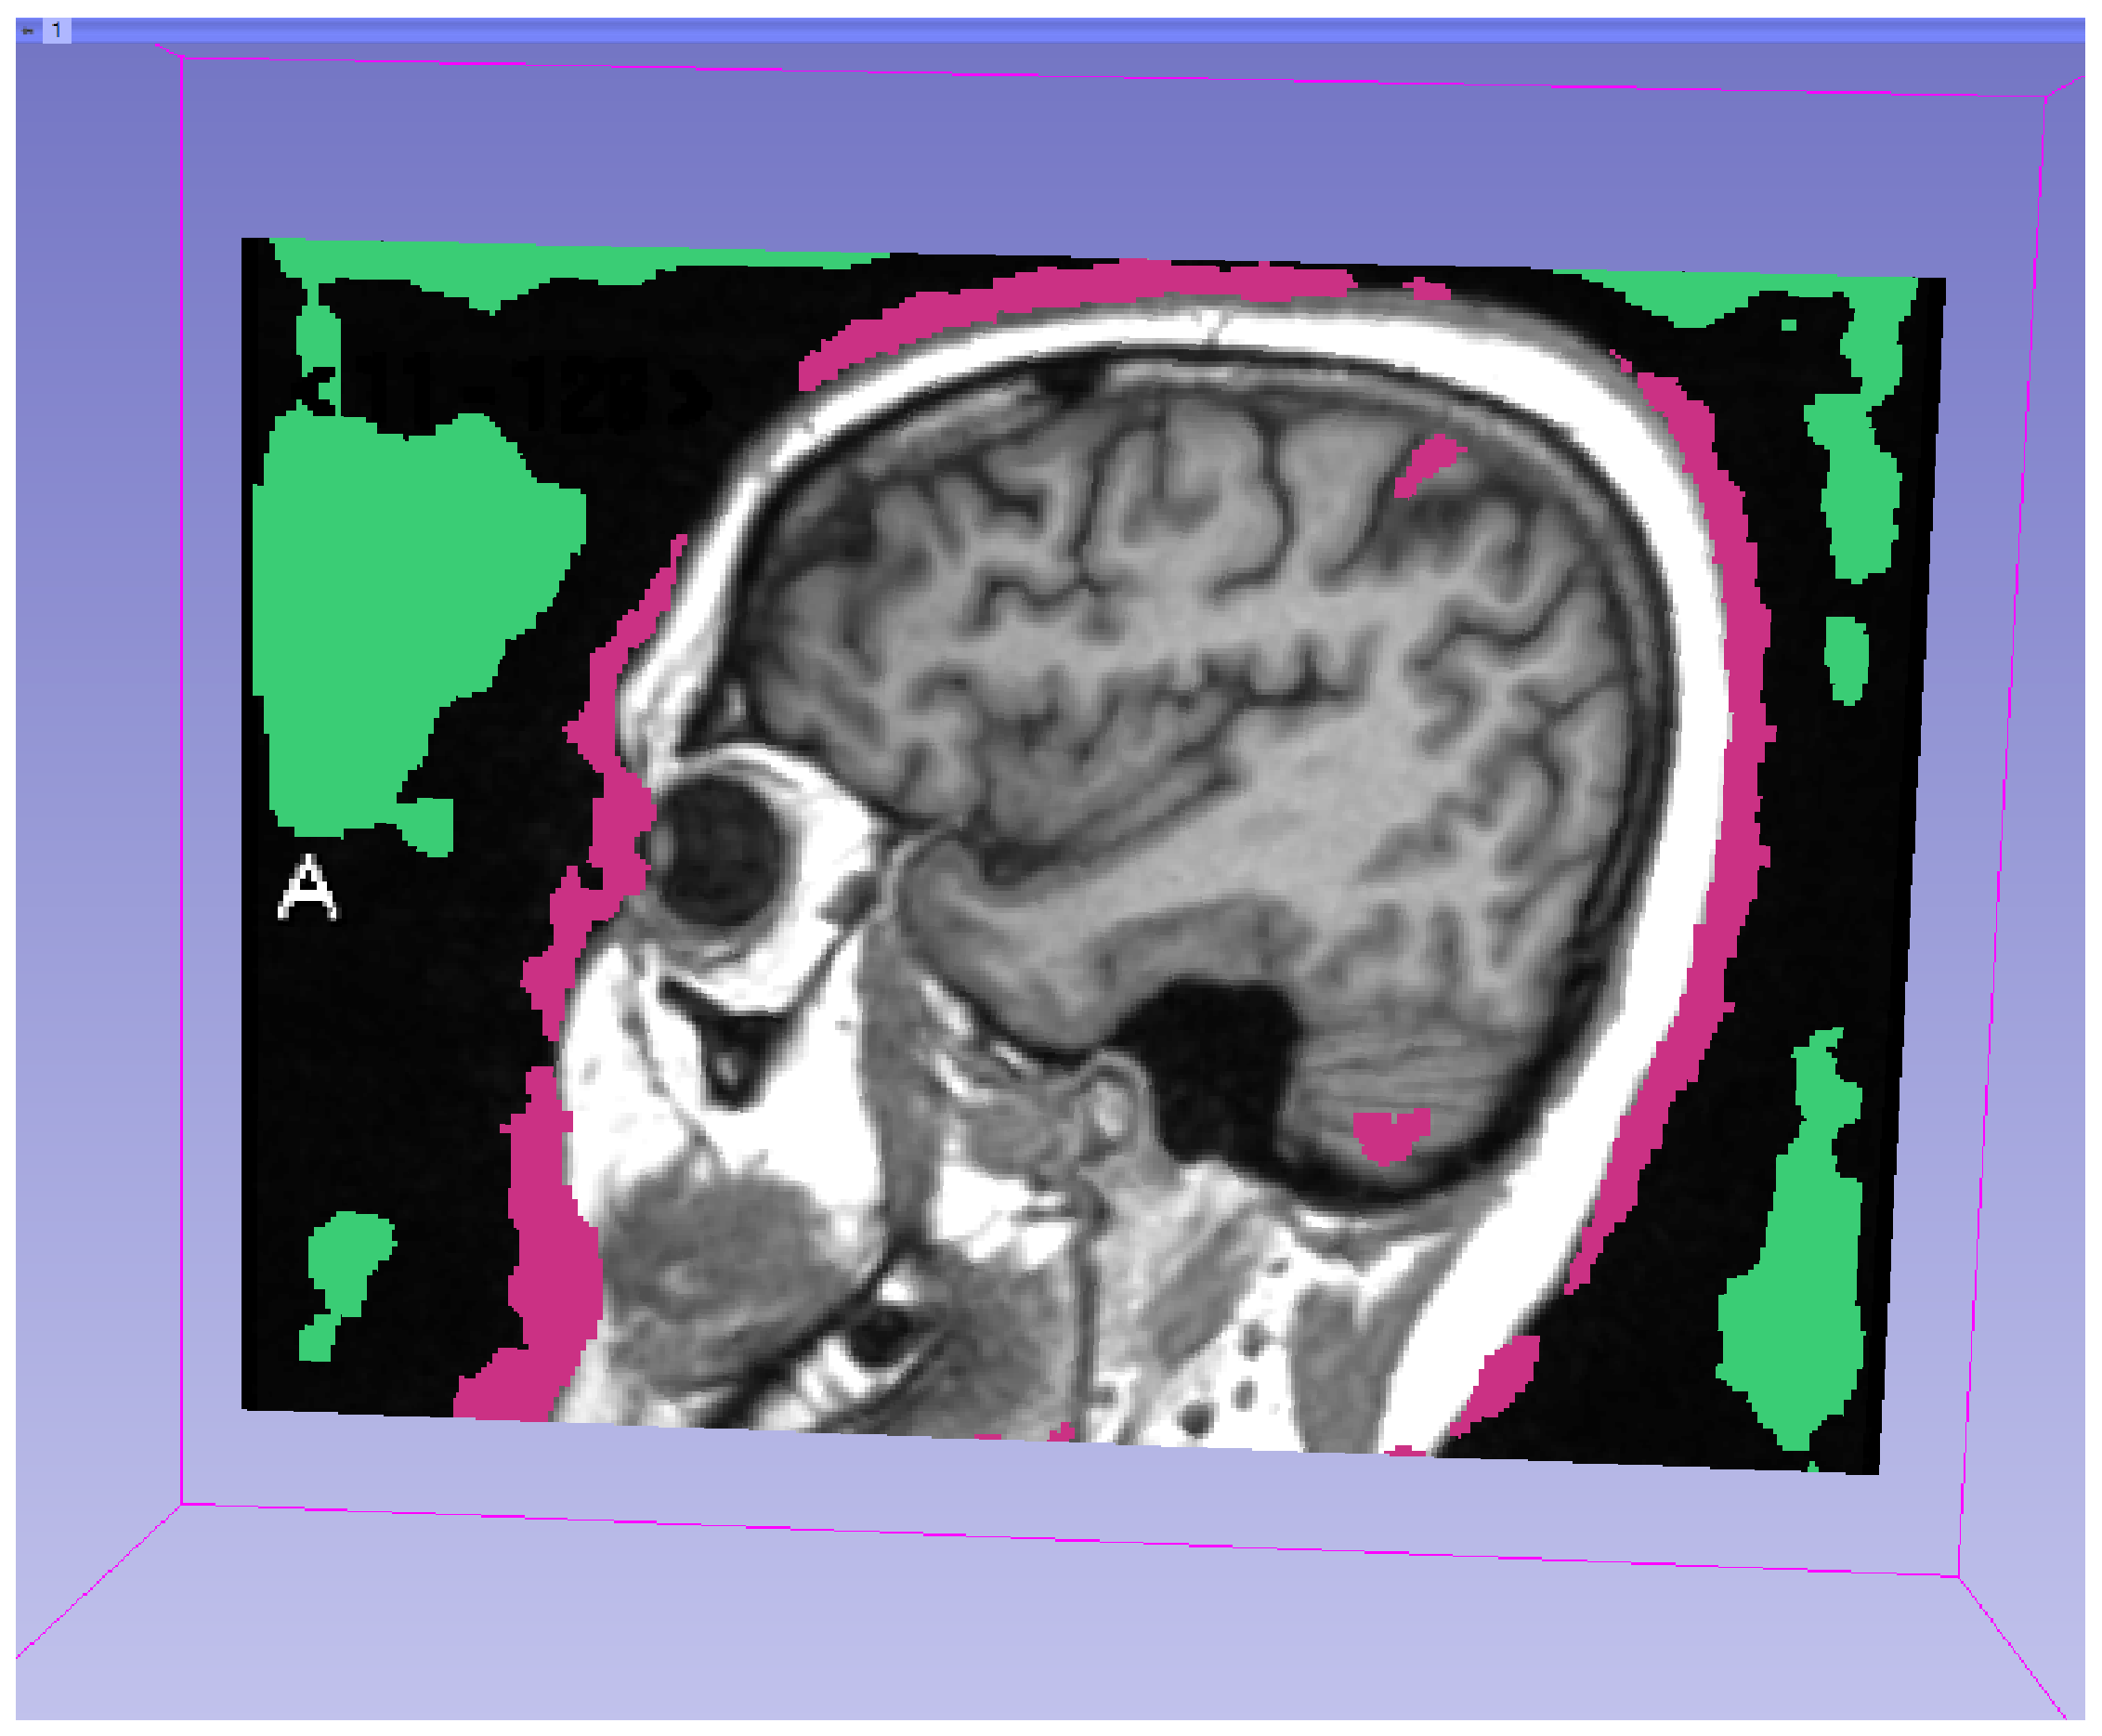
\includegraphics[scale=0.2]{/experiment_CL_P1/CL_Tensor_Sagittal.eps}
  \caption{Tensor-based method. Patient 1: Sagittal plane}
  \label{CL_TSagittal}
\end{figure}


\subsection{Patient 2}
The differences in this patient, if actually present, are really
small. 

\subsubsection{Voxel-based Method}
The voxel-based method shows small differences near the corpus
callosum on the three planes; this differences, accourding to the
medical expert, might be real because this is a very common area
affected by trauma.\\

The registration method used was \textit{Affine registration}.

\begin{figure}[H]
  \centering
  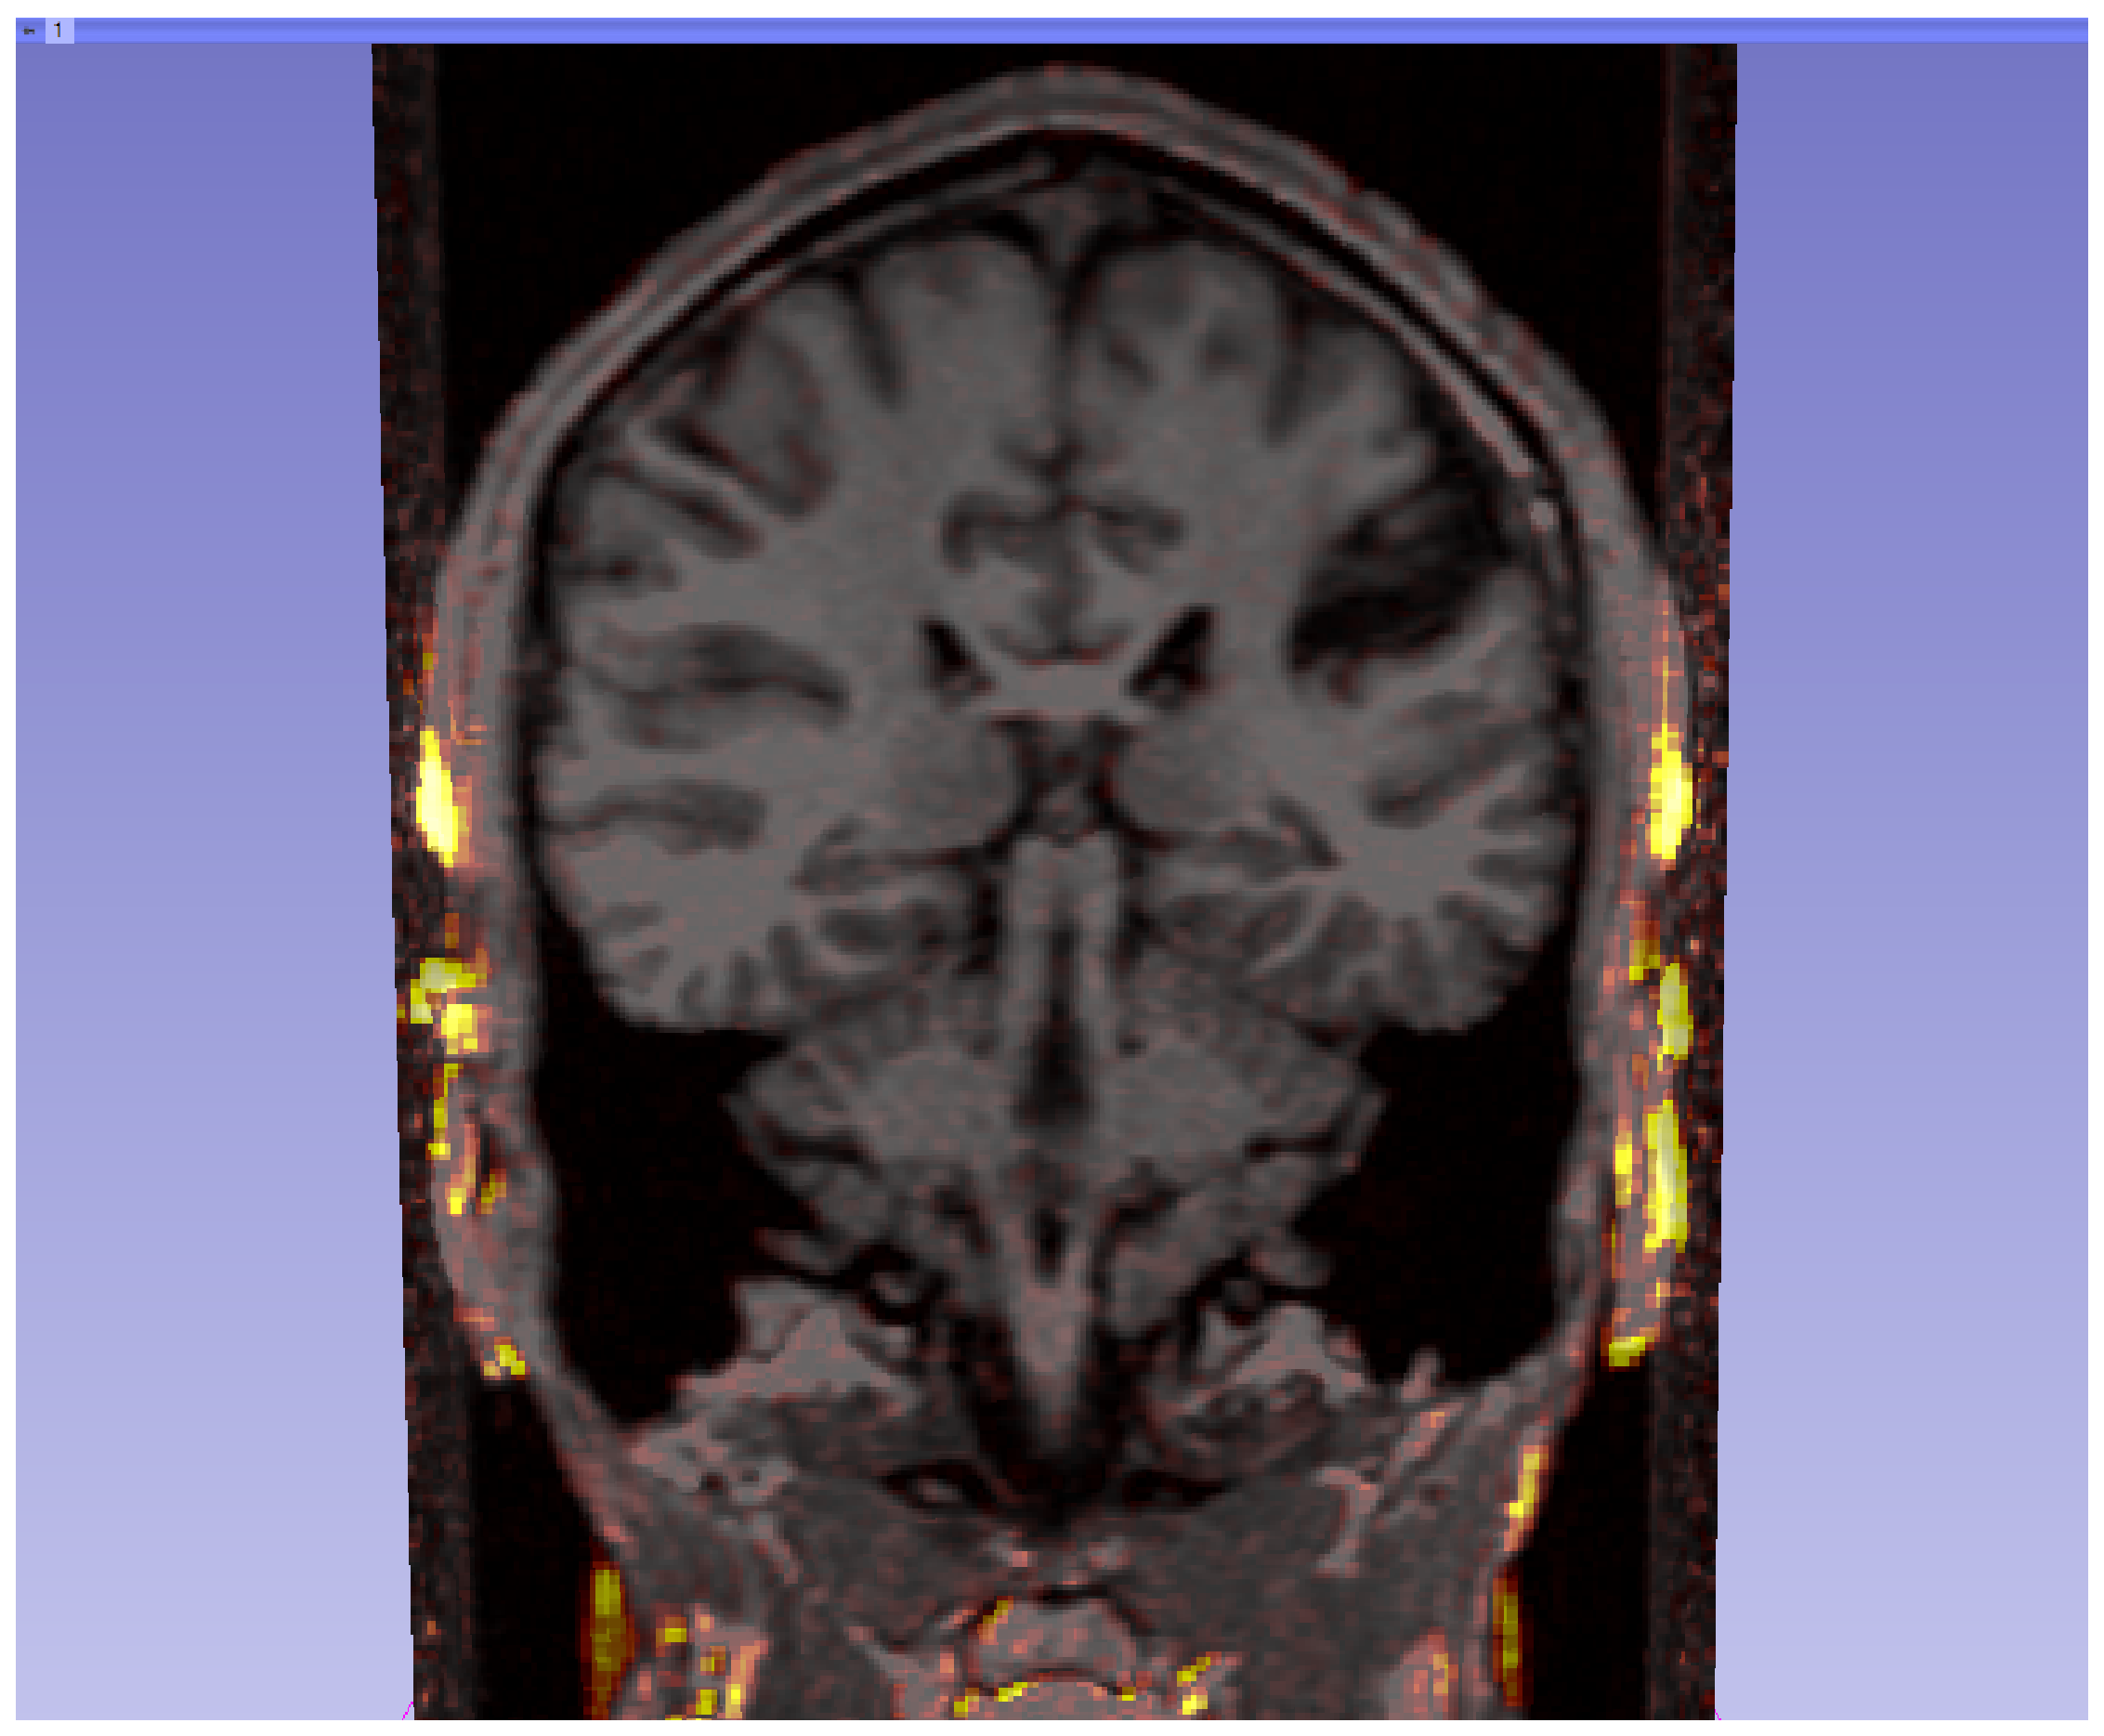
\includegraphics[scale=0.2]{/experiment_PB_P2/PB_Coronal.eps}
  \caption{Voxel-based method. Patient 2: Coronal plane}
  \label{PB_Coronal}
\end{figure}

\begin{figure}[H]
  \centering
  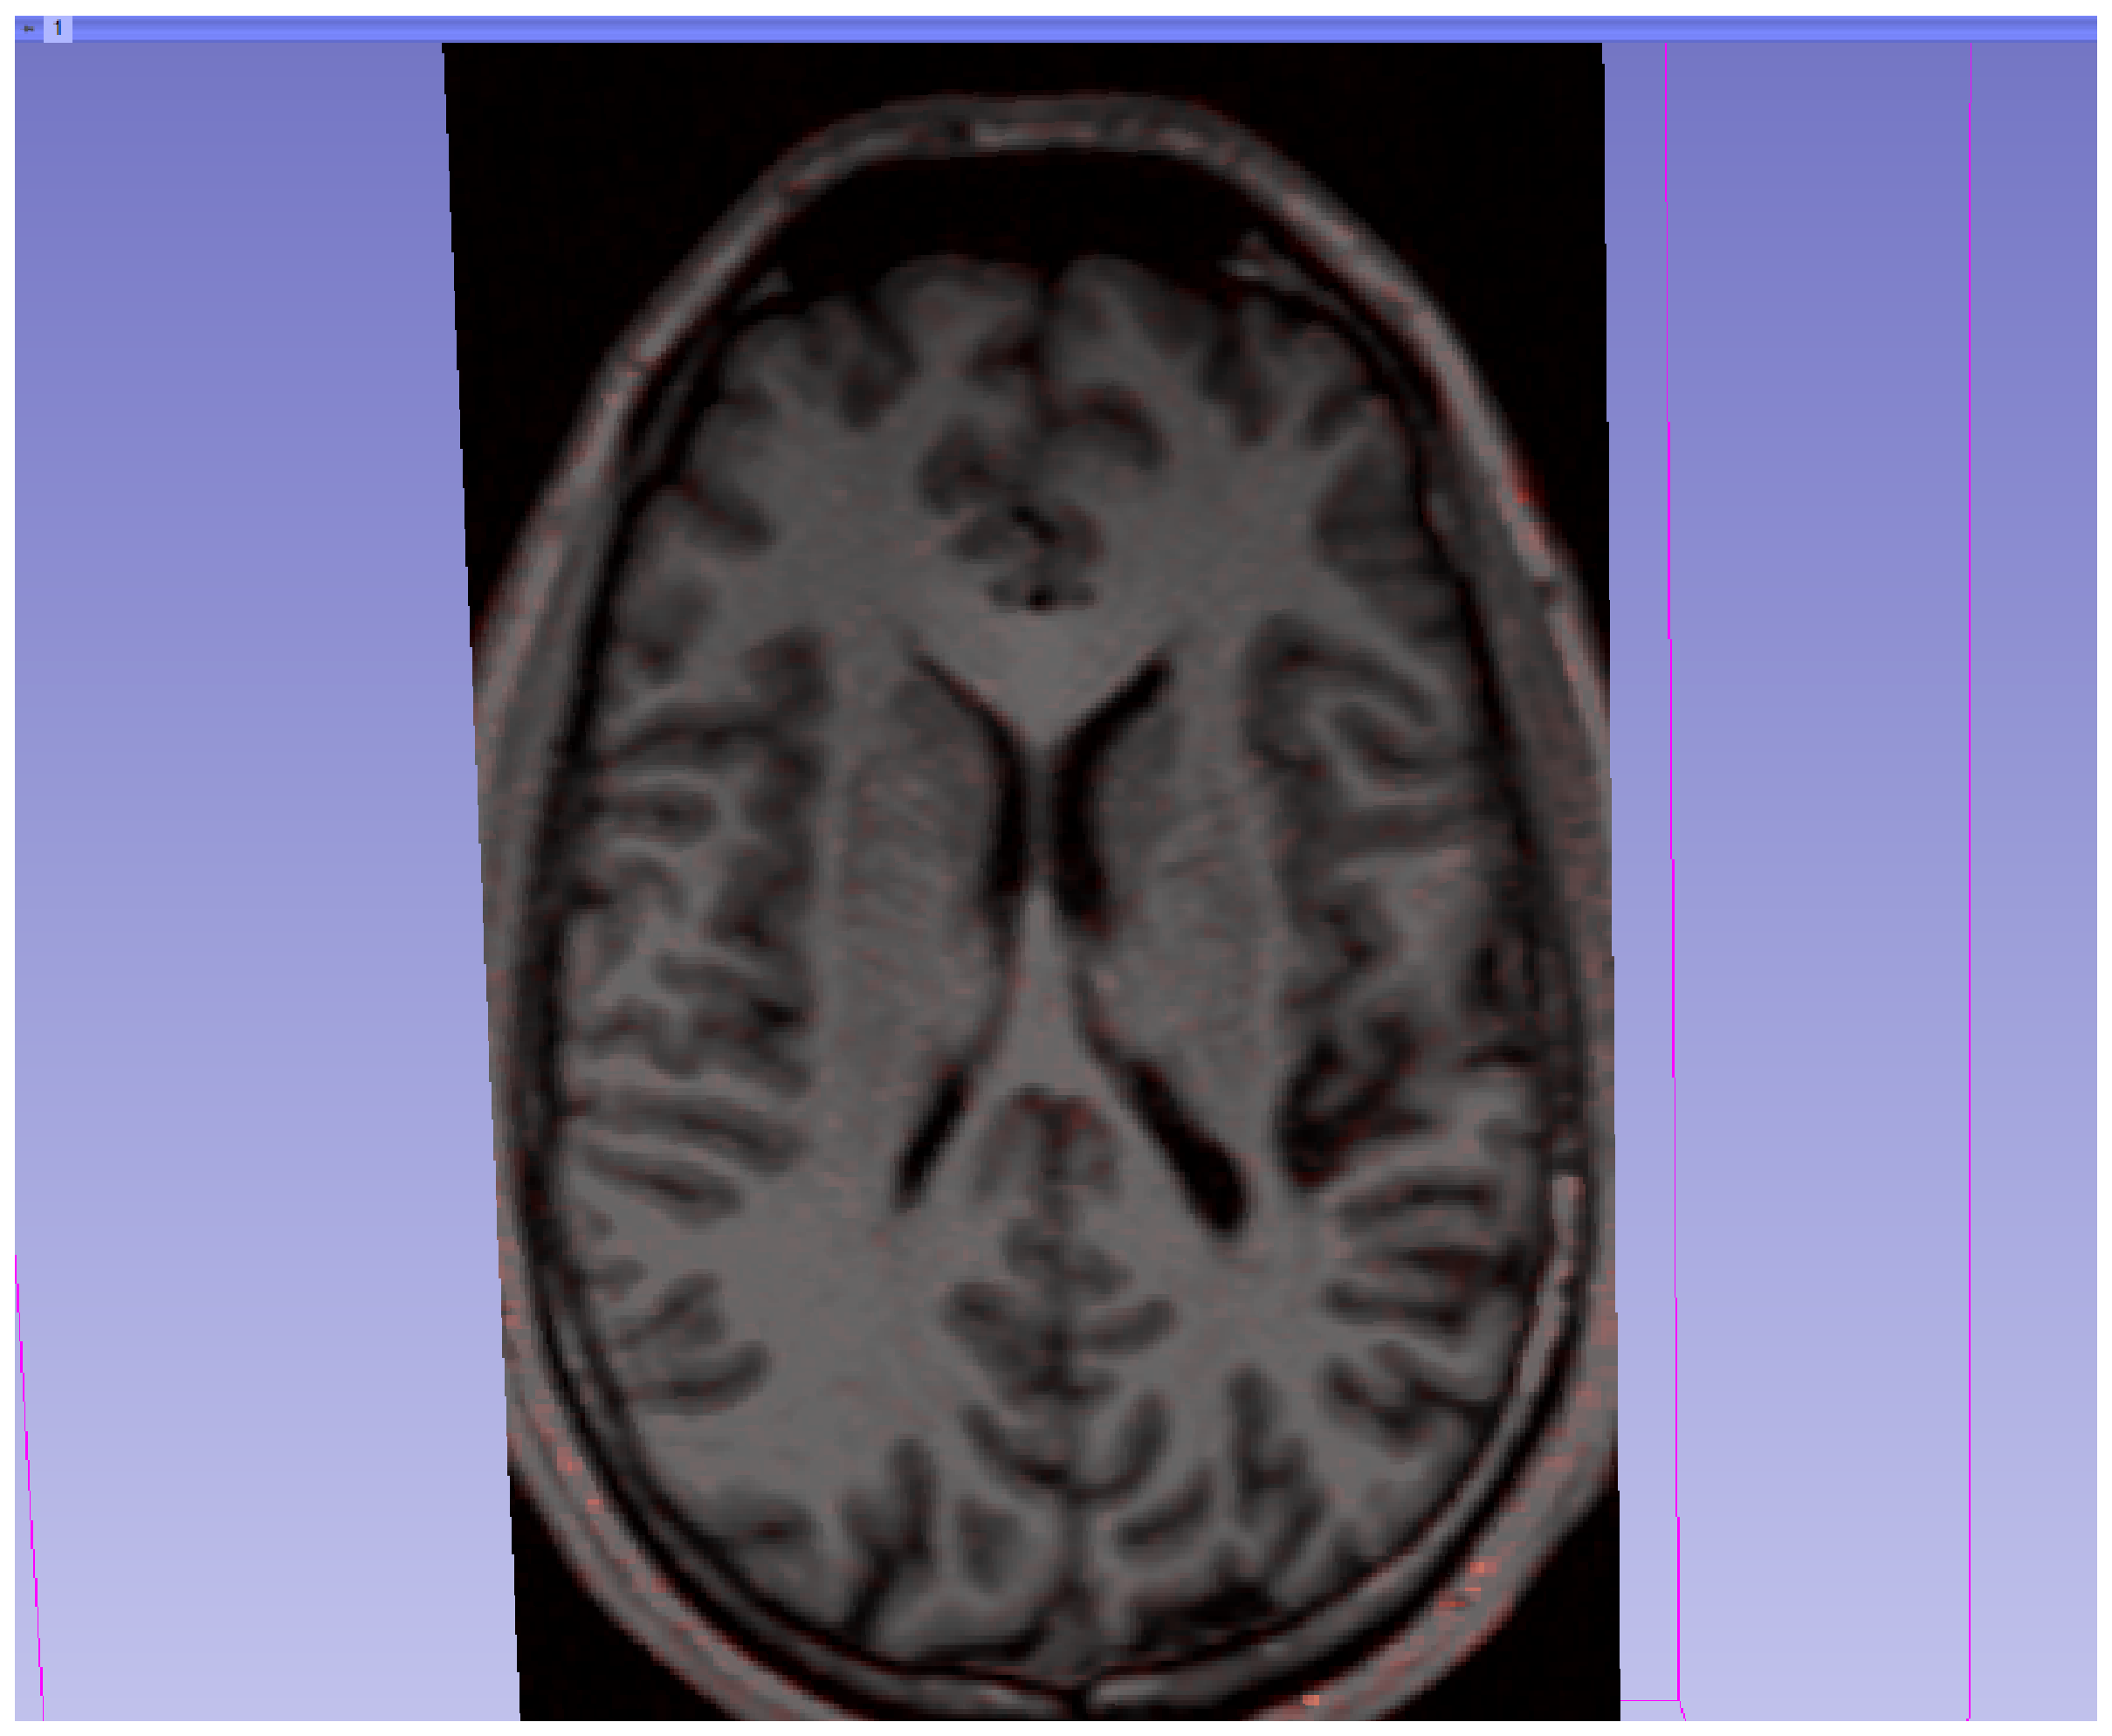
\includegraphics[scale=0.2]{/experiment_PB_P2/PB_Traversal.eps}
  \caption{Voxel-based method. Patient 2: Traversal plane}
  \label{PB_Traversal}
\end{figure}

\begin{figure}[H]
  \centering
  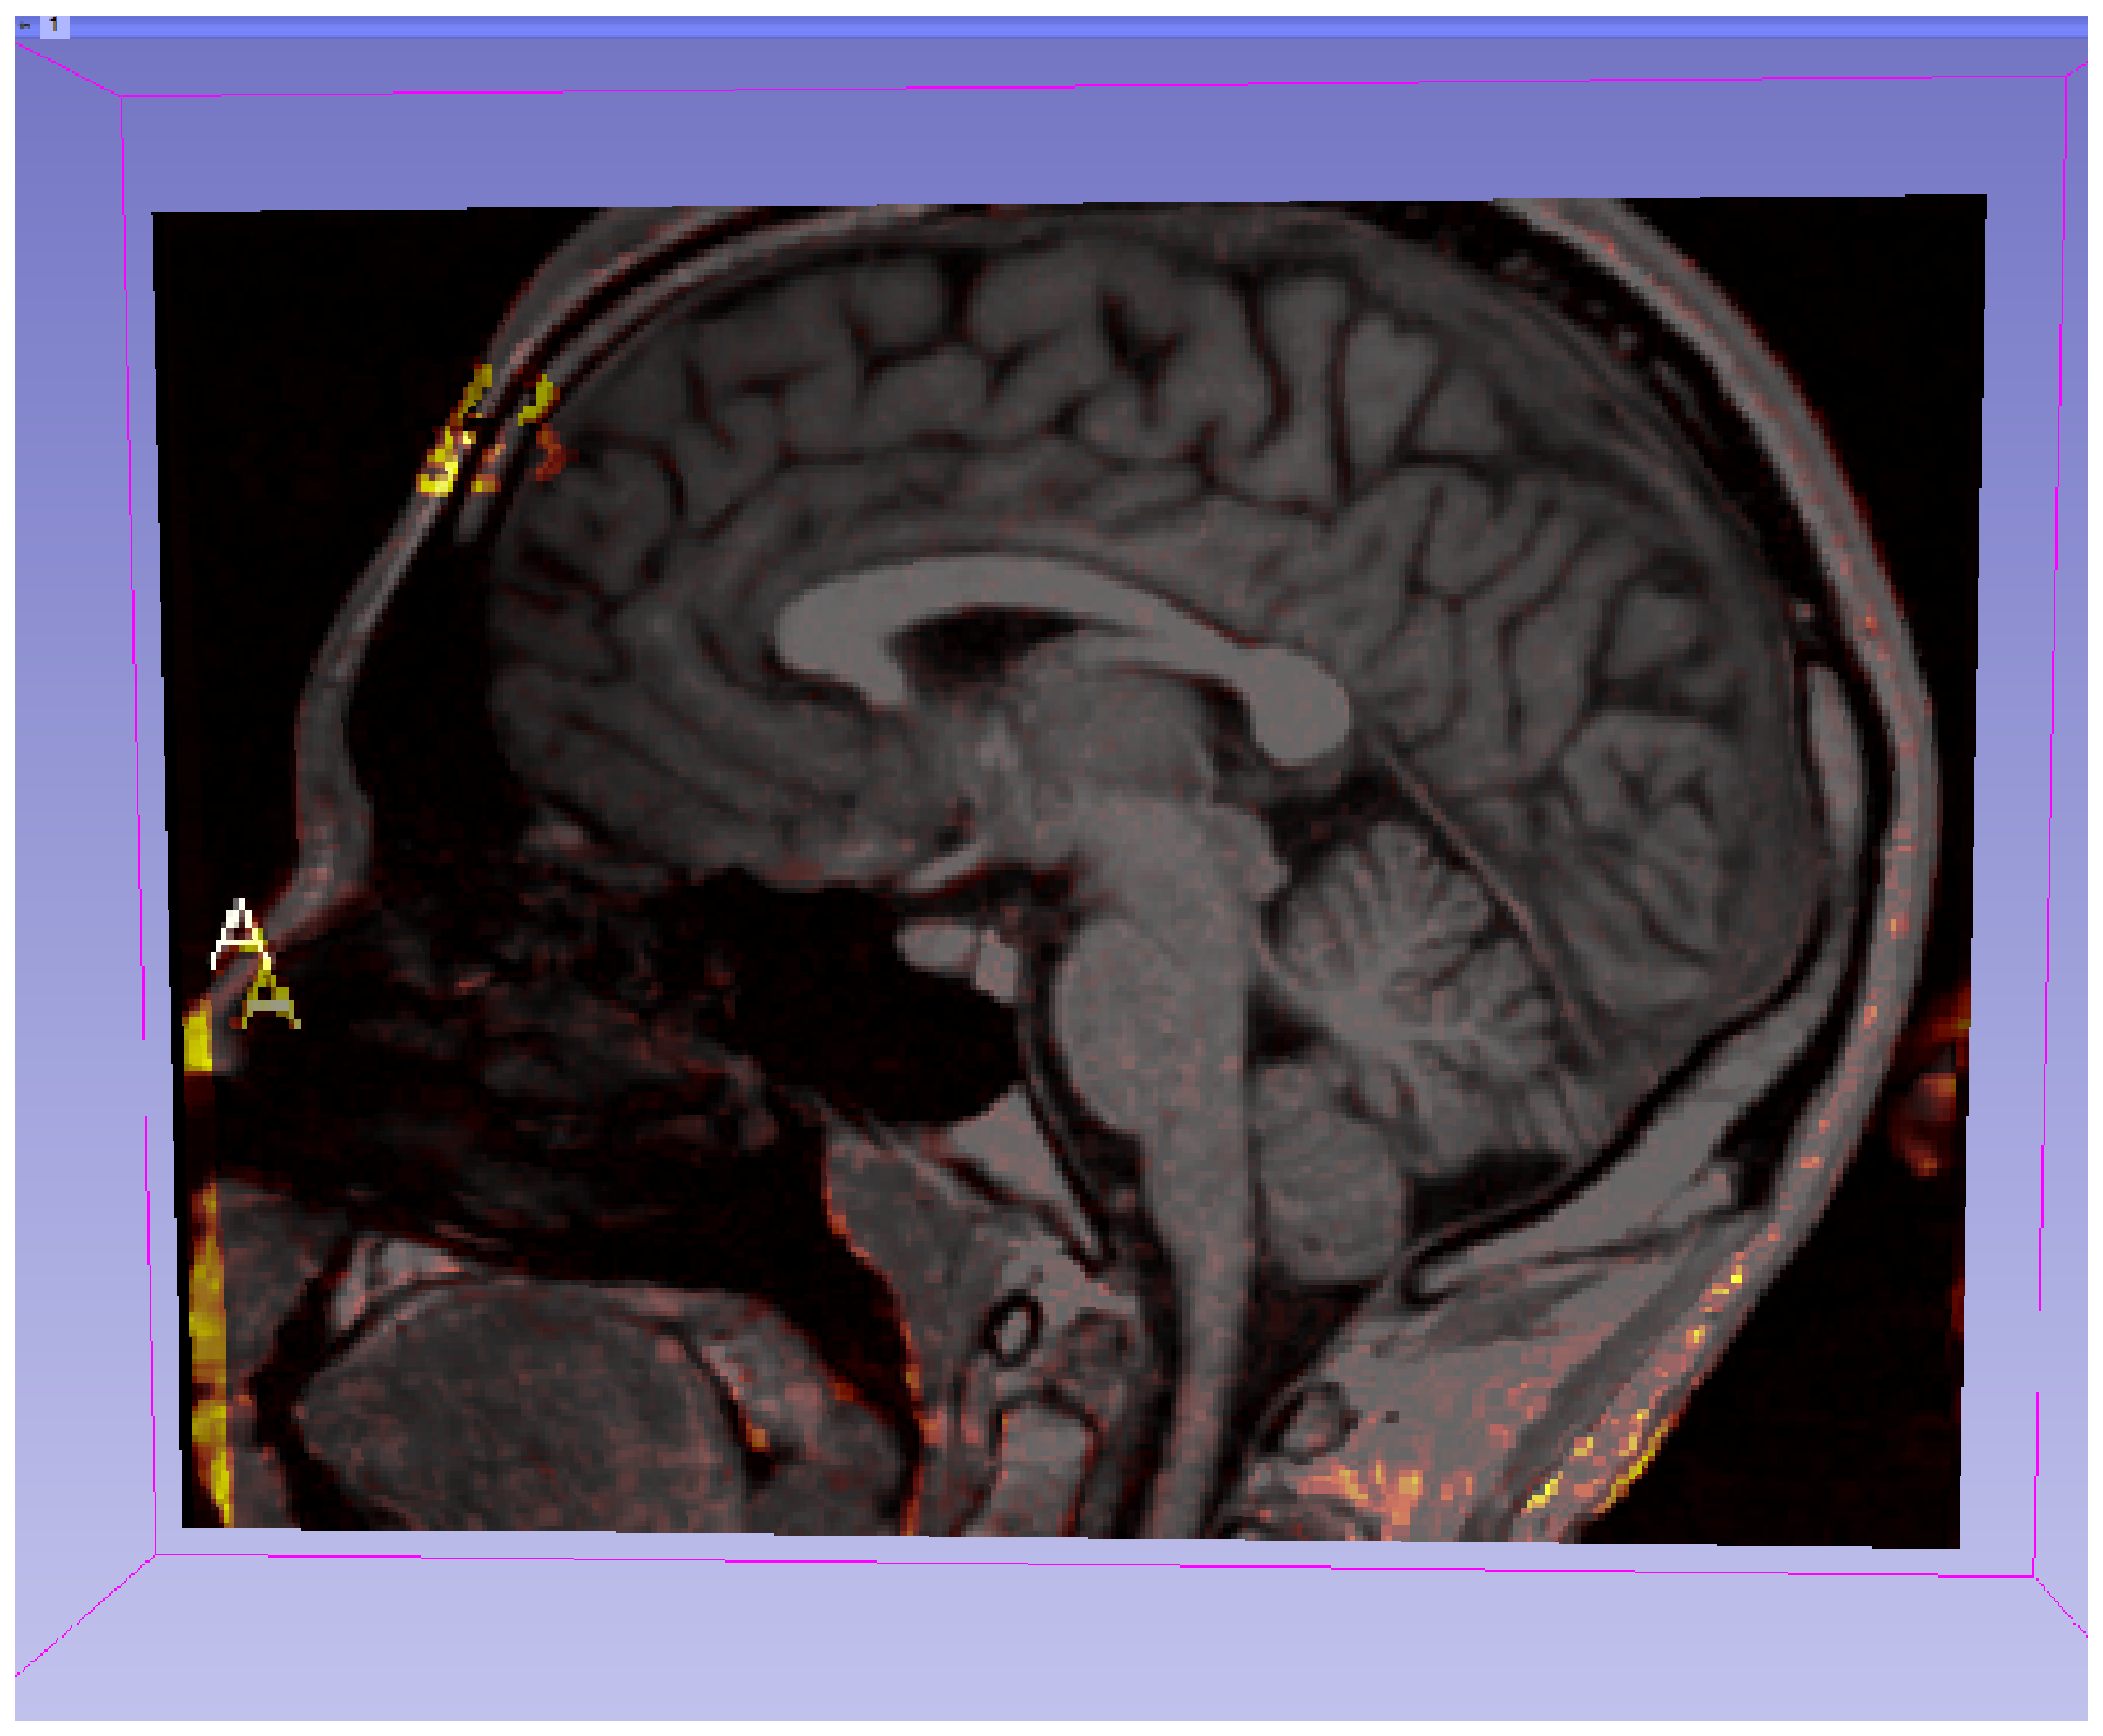
\includegraphics[scale=0.2]{/experiment_PB_P2/PB_Sagittal.eps}
  \caption{Voxel-based method. Patient 2: Sagittal plane}
  \label{PB_Sagittal}
\end{figure}


\subsubsection{Tensor-based Method}
The tensor-base method doesn't find the same differences in the corpus
callosum as the previous method. With the usual percentage values
(from $70\%$ to $80\%$ for both growth and shrinkage), the method almost
doesn't find any differences. 

In order to show some of the possible places where the method shows
some type of differences, the value of the shrinkage percentage was
increased until $88\%$. Given this, the pink areas shown are not
necessarily real differences.\\

Parameters used:
\begin{description}
\item \textit{Deformation field smoothing sigma:} 2.5
\item \textit{Shrinkage percentage:} 80
\item \textit{Growth percentage:} 88
\end{description}

\begin{figure}[H]
  \centering
  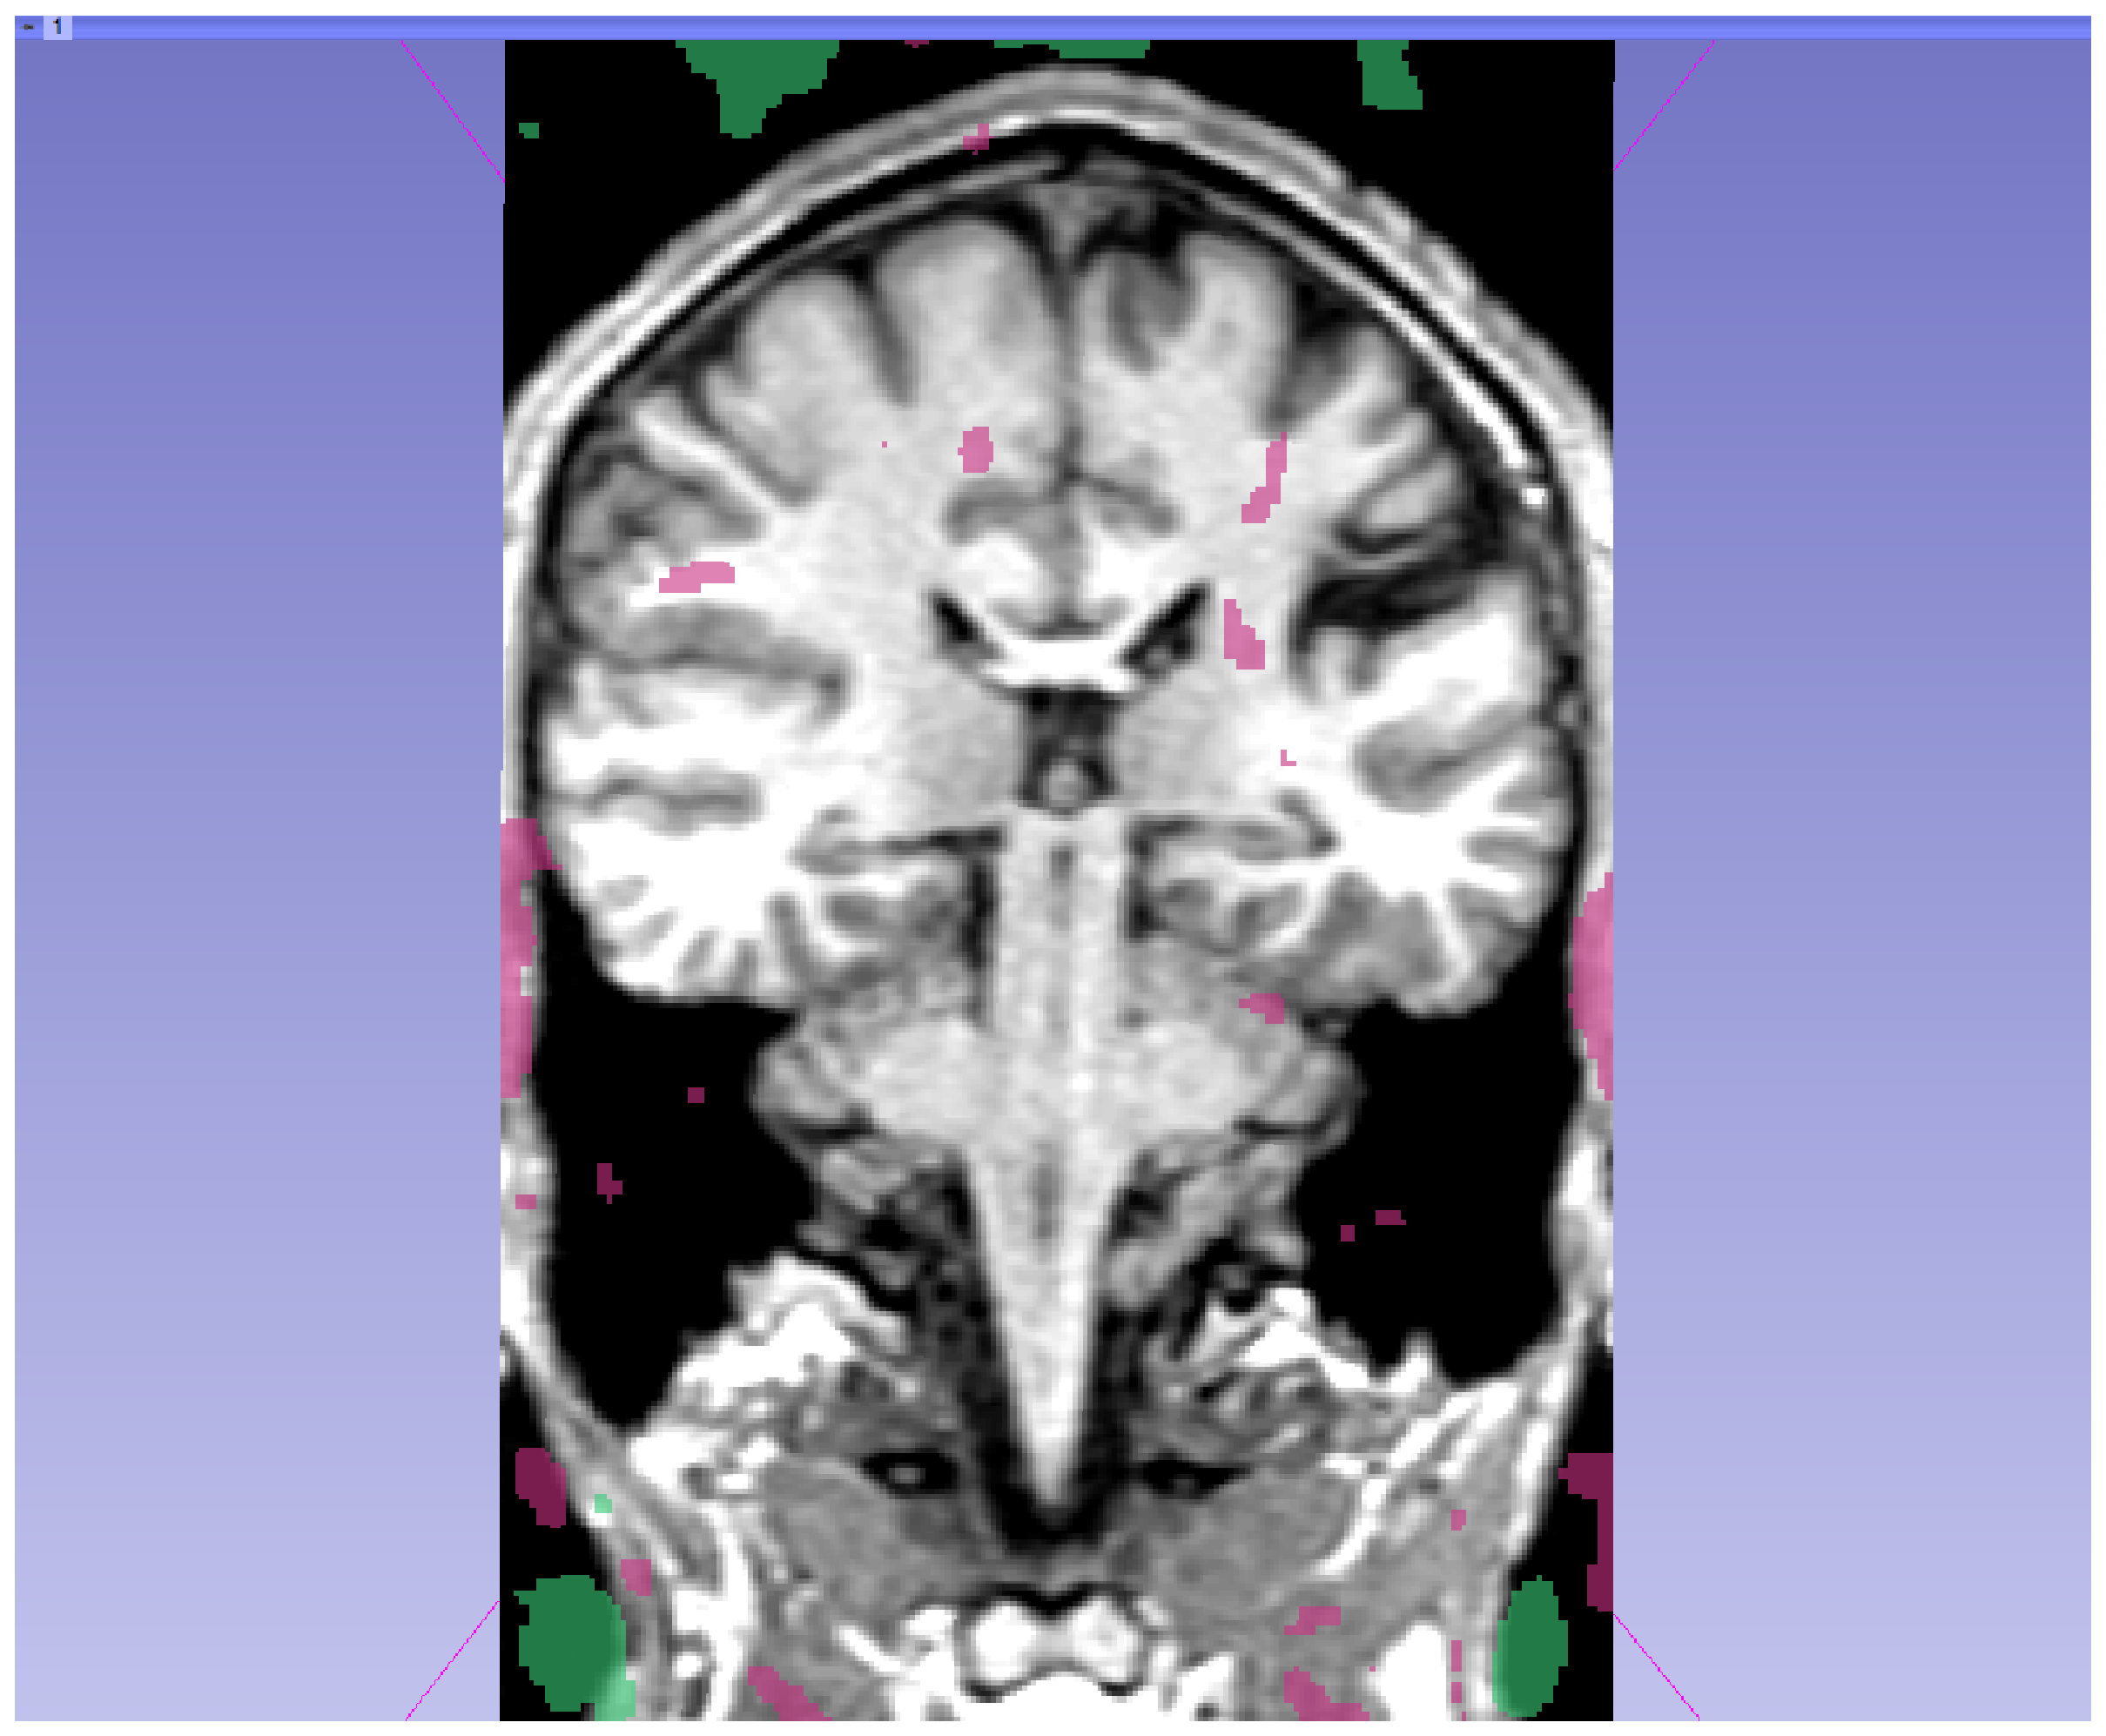
\includegraphics[scale=0.2]{/experiment_PB_P2/PB_Tensor_Coronal.eps}
  \caption{Tensor-based method. Patient 2: Coronal plane}
  \label{PB_TCoronal}
\end{figure}

\begin{figure}[H]
  \centering
  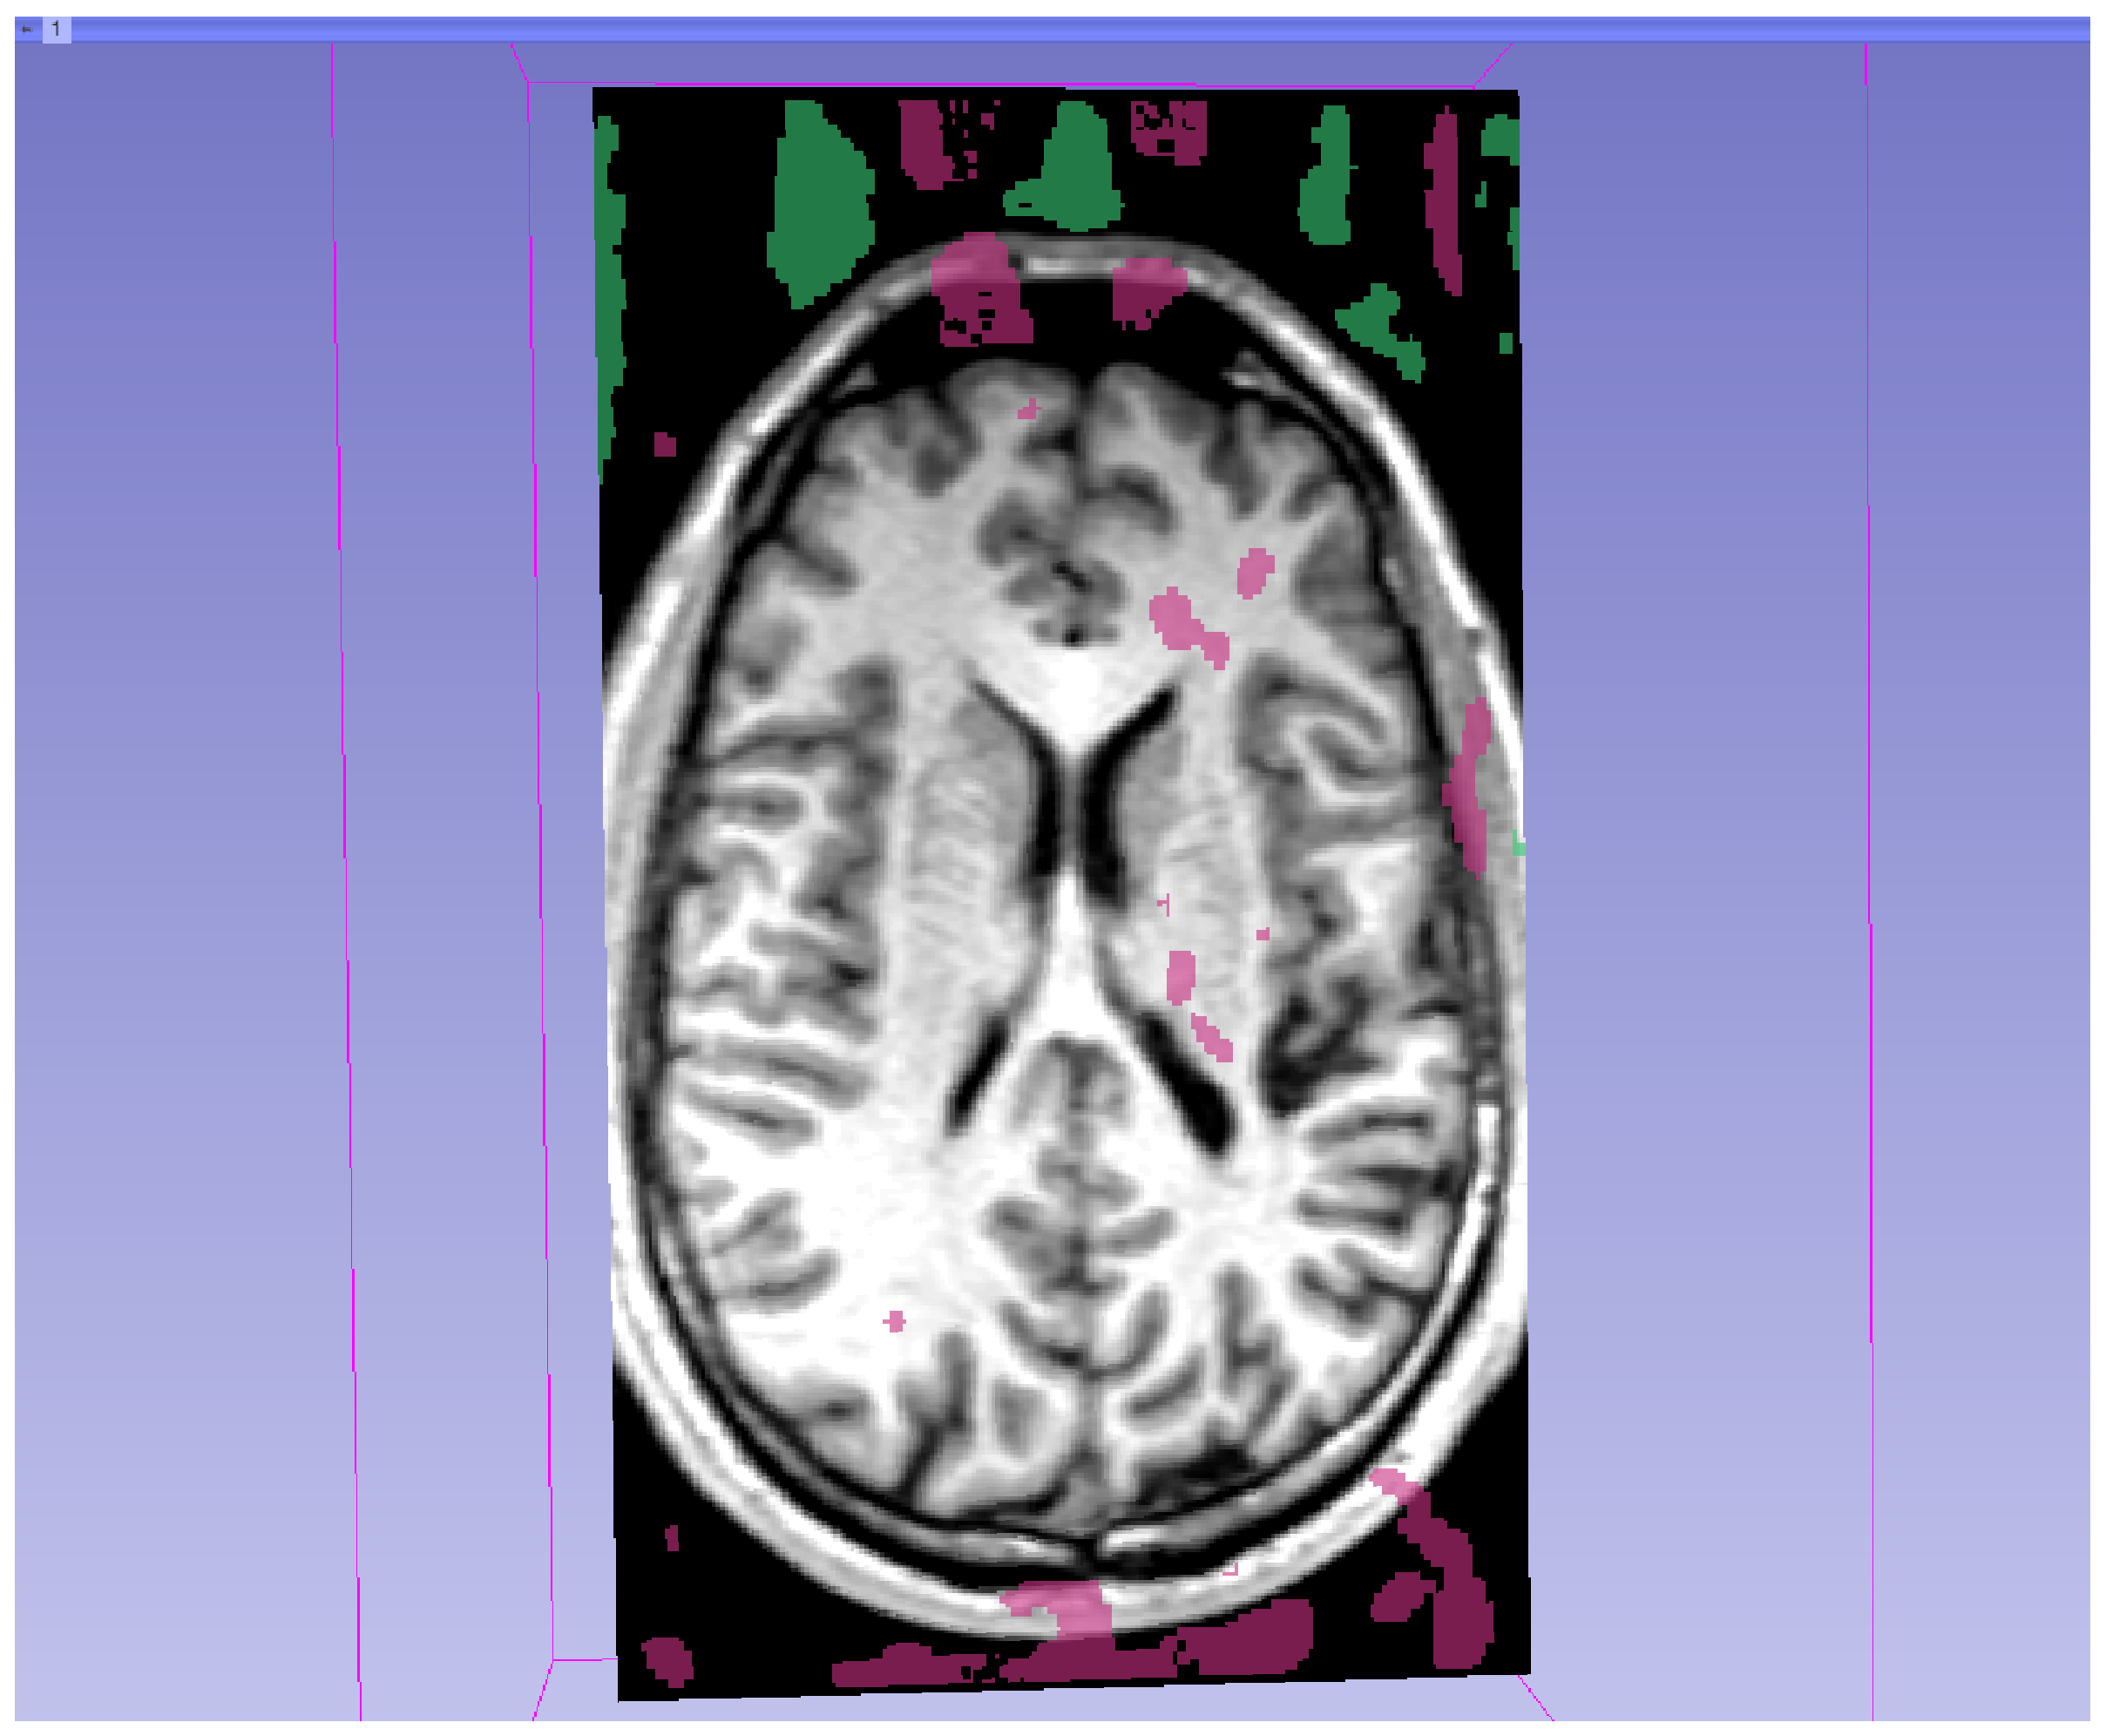
\includegraphics[scale=0.2]{/experiment_PB_P2/PB_Tensor_Traversal.eps}
  \caption{Tensor-based method. Patient 2: Traversal plane}
  \label{PB_TTraversal}
\end{figure}

\begin{figure}[H]
  \centering
  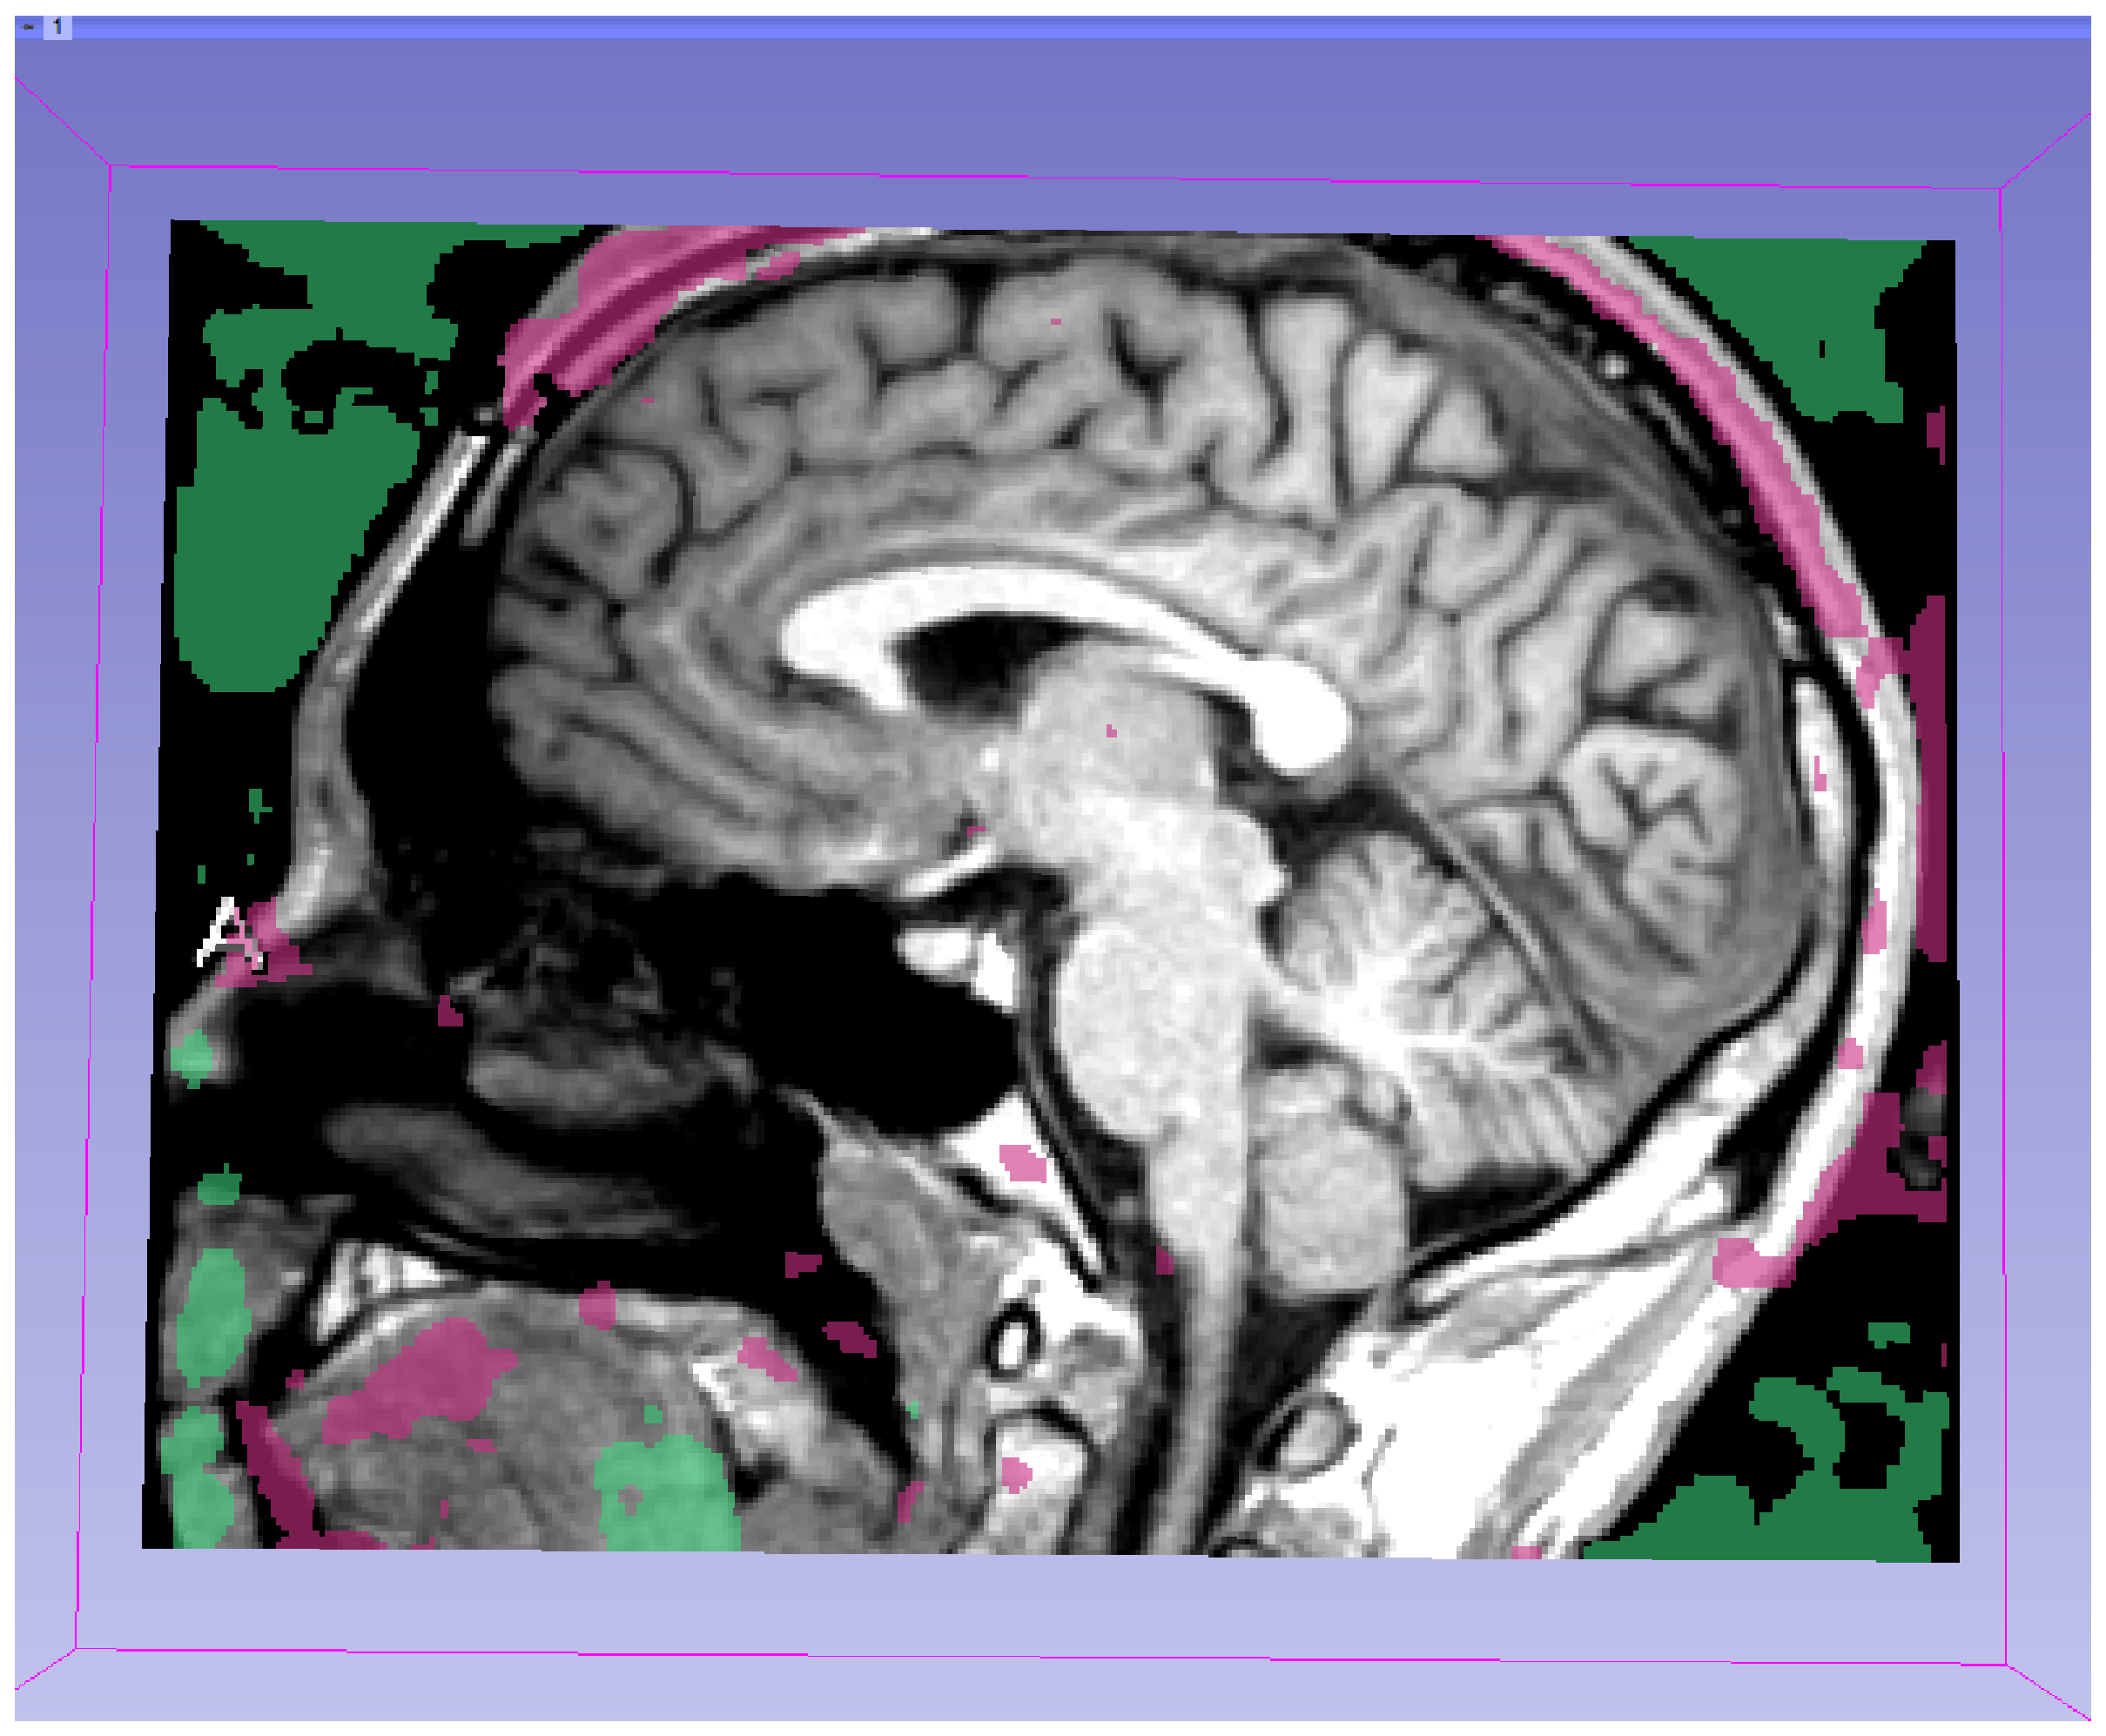
\includegraphics[scale=0.2]{/experiment_PB_P2/PB_Tensor_Sagittal.eps}
  \caption{Tensor-based method. Patient 2: Sagittal plane}
  \label{PB_TSagittal}
\end{figure}


\subsection{Patient 3}
This patient had a medical condition for which it has had two
surgeries performed. A tumor, located on the right hemisphere of the
frontal lobe, was removed during the first surgery. The MRIs used
during this experiment were taken before and after the second surgery,
in which a second growth was removed located the same area.


\subsubsection{Voxel-based Method}
The method shows the expected differences in the right hemisphere of
the frontal lobe of the brain. It also shows some size differences
especially in the lower parietal lobe, which can be observed in image
\ref{B2_Traversal1}.\\

The registration method used was \textit{Affine registration}.

\begin{figure}[H]
  \centering
  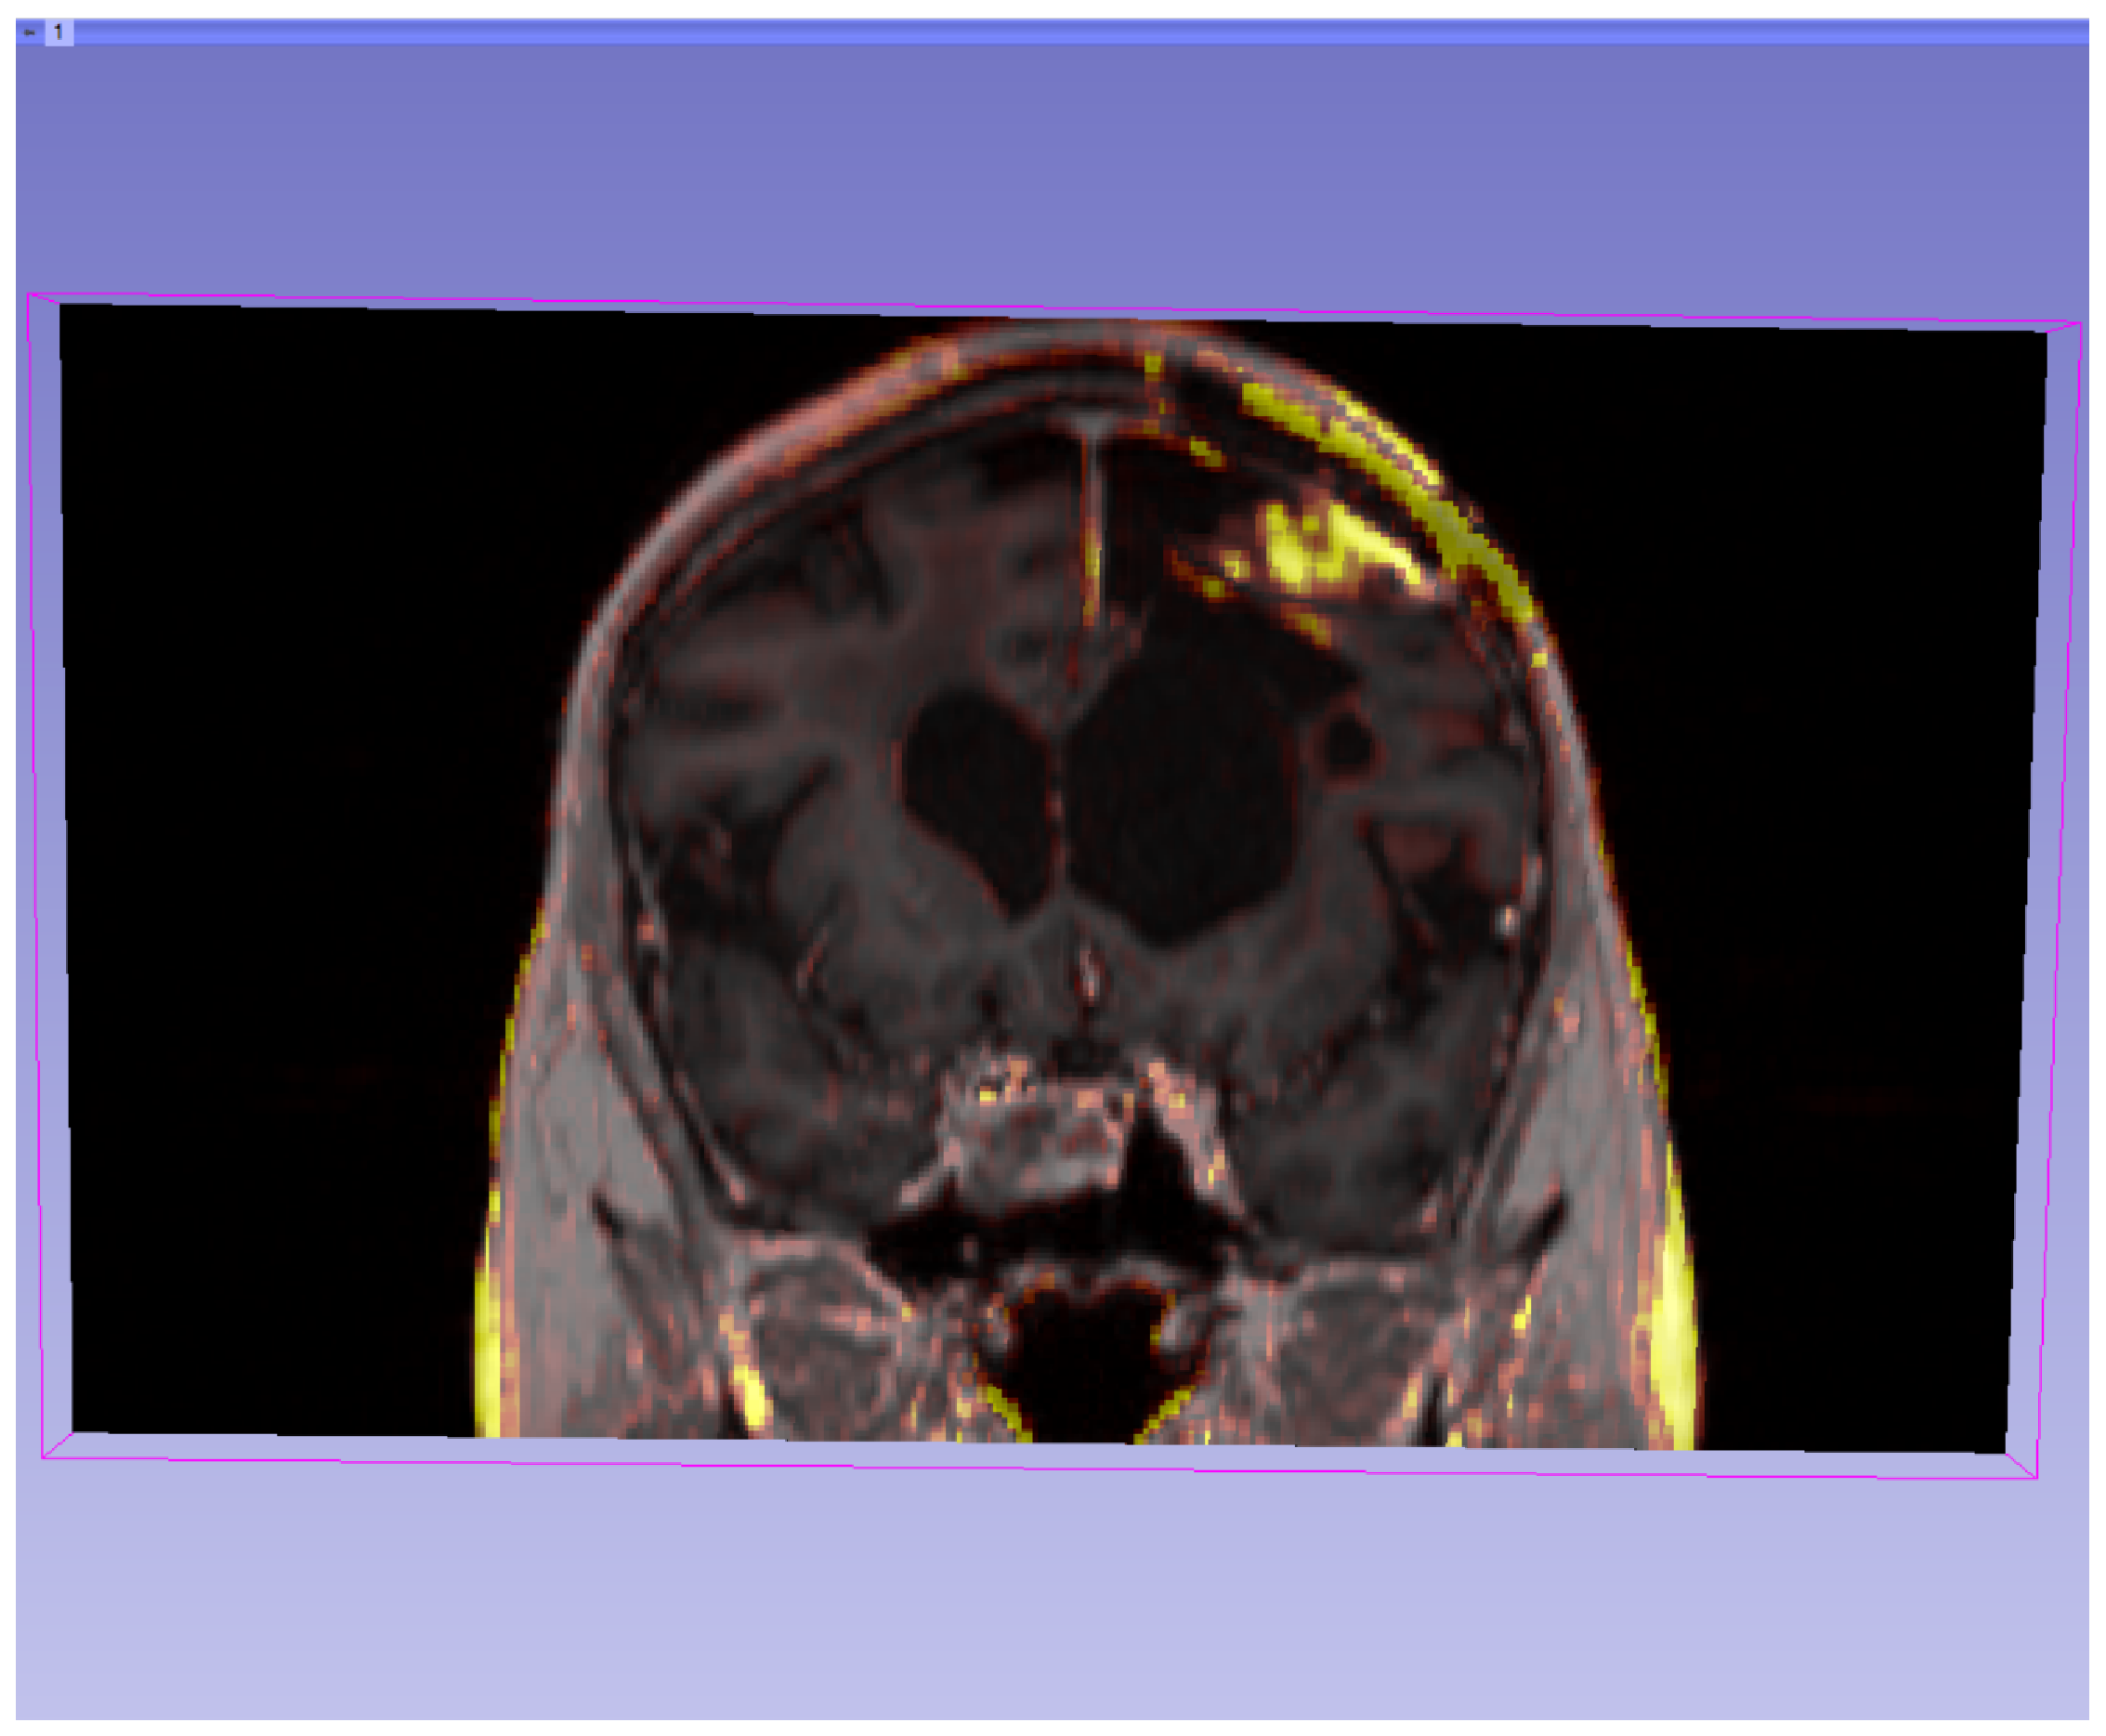
\includegraphics[scale=0.2]{/experiment_B2_P3/B2_Coronal.eps}
  \caption{Voxel-based method. Patient 3: Coronal plane}
  \label{B2_Coronal}
\end{figure}

\begin{figure}[H]
  \centering
  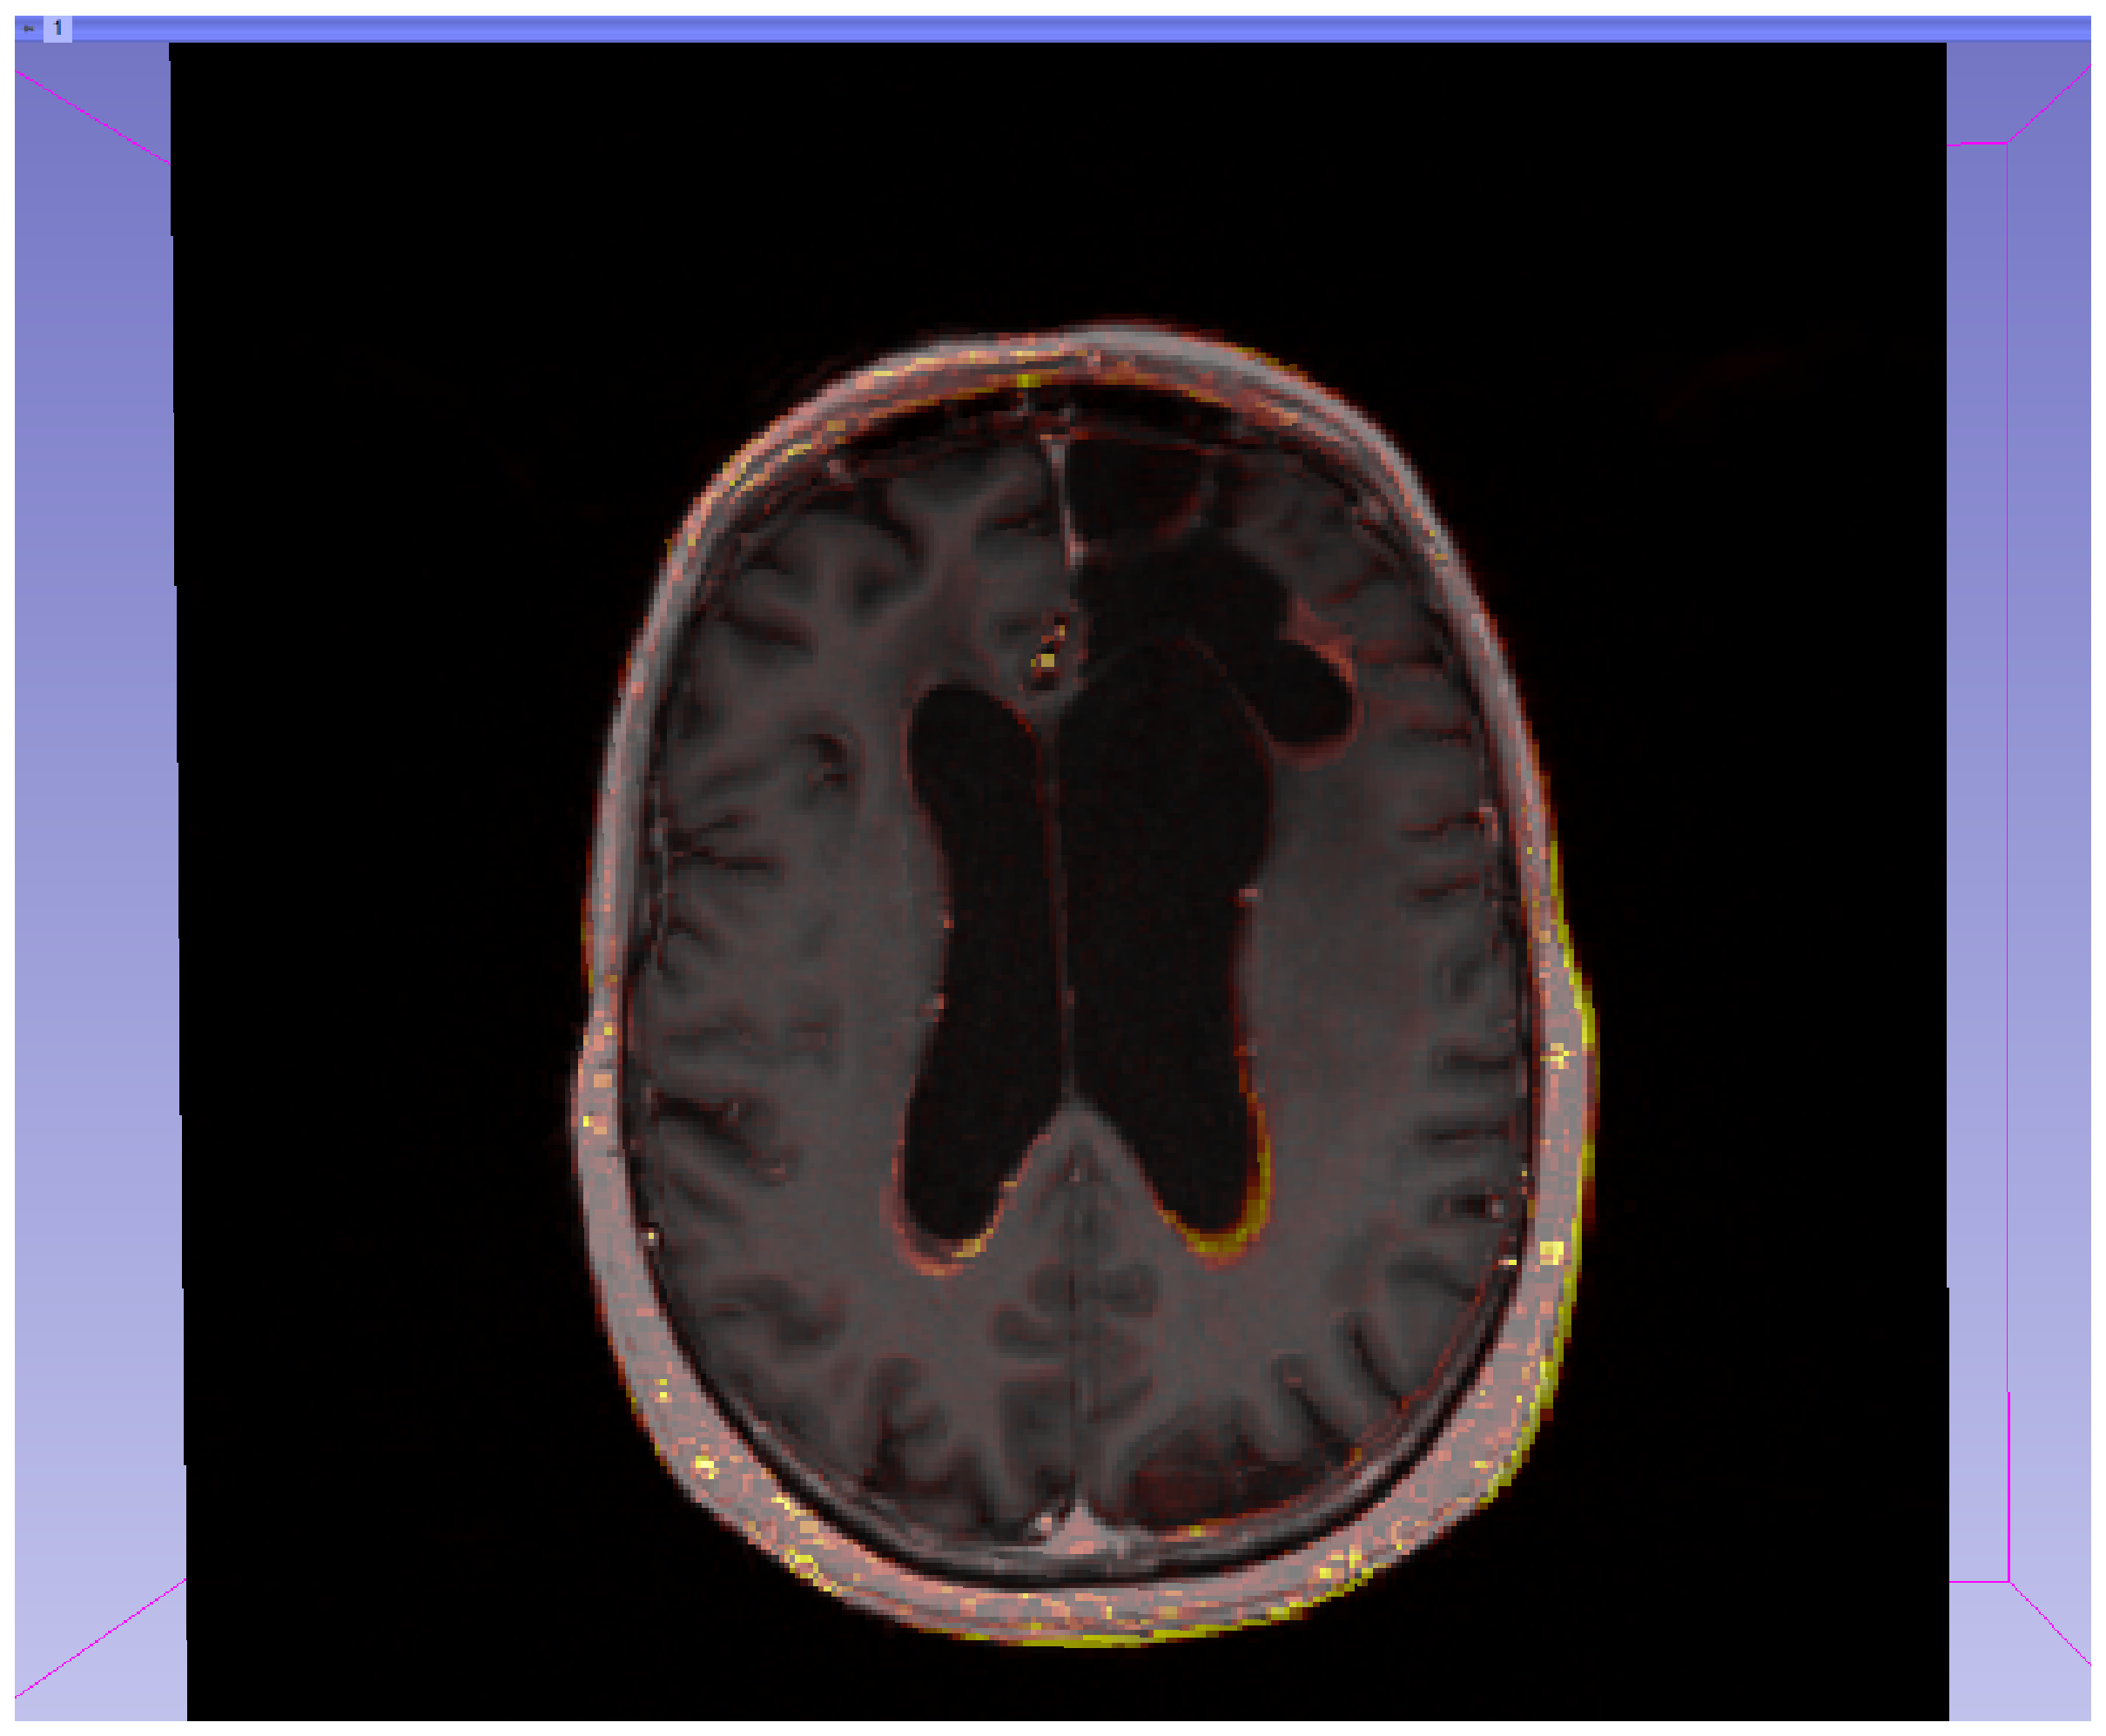
\includegraphics[scale=0.2]{/experiment_B2_P3/B2_Traversal1.eps}
  \caption{Voxel-based method. Patient 3: Traversal plane}
  \label{B2_Traversal1}
\end{figure}

\begin{figure}[H]
  \centering
  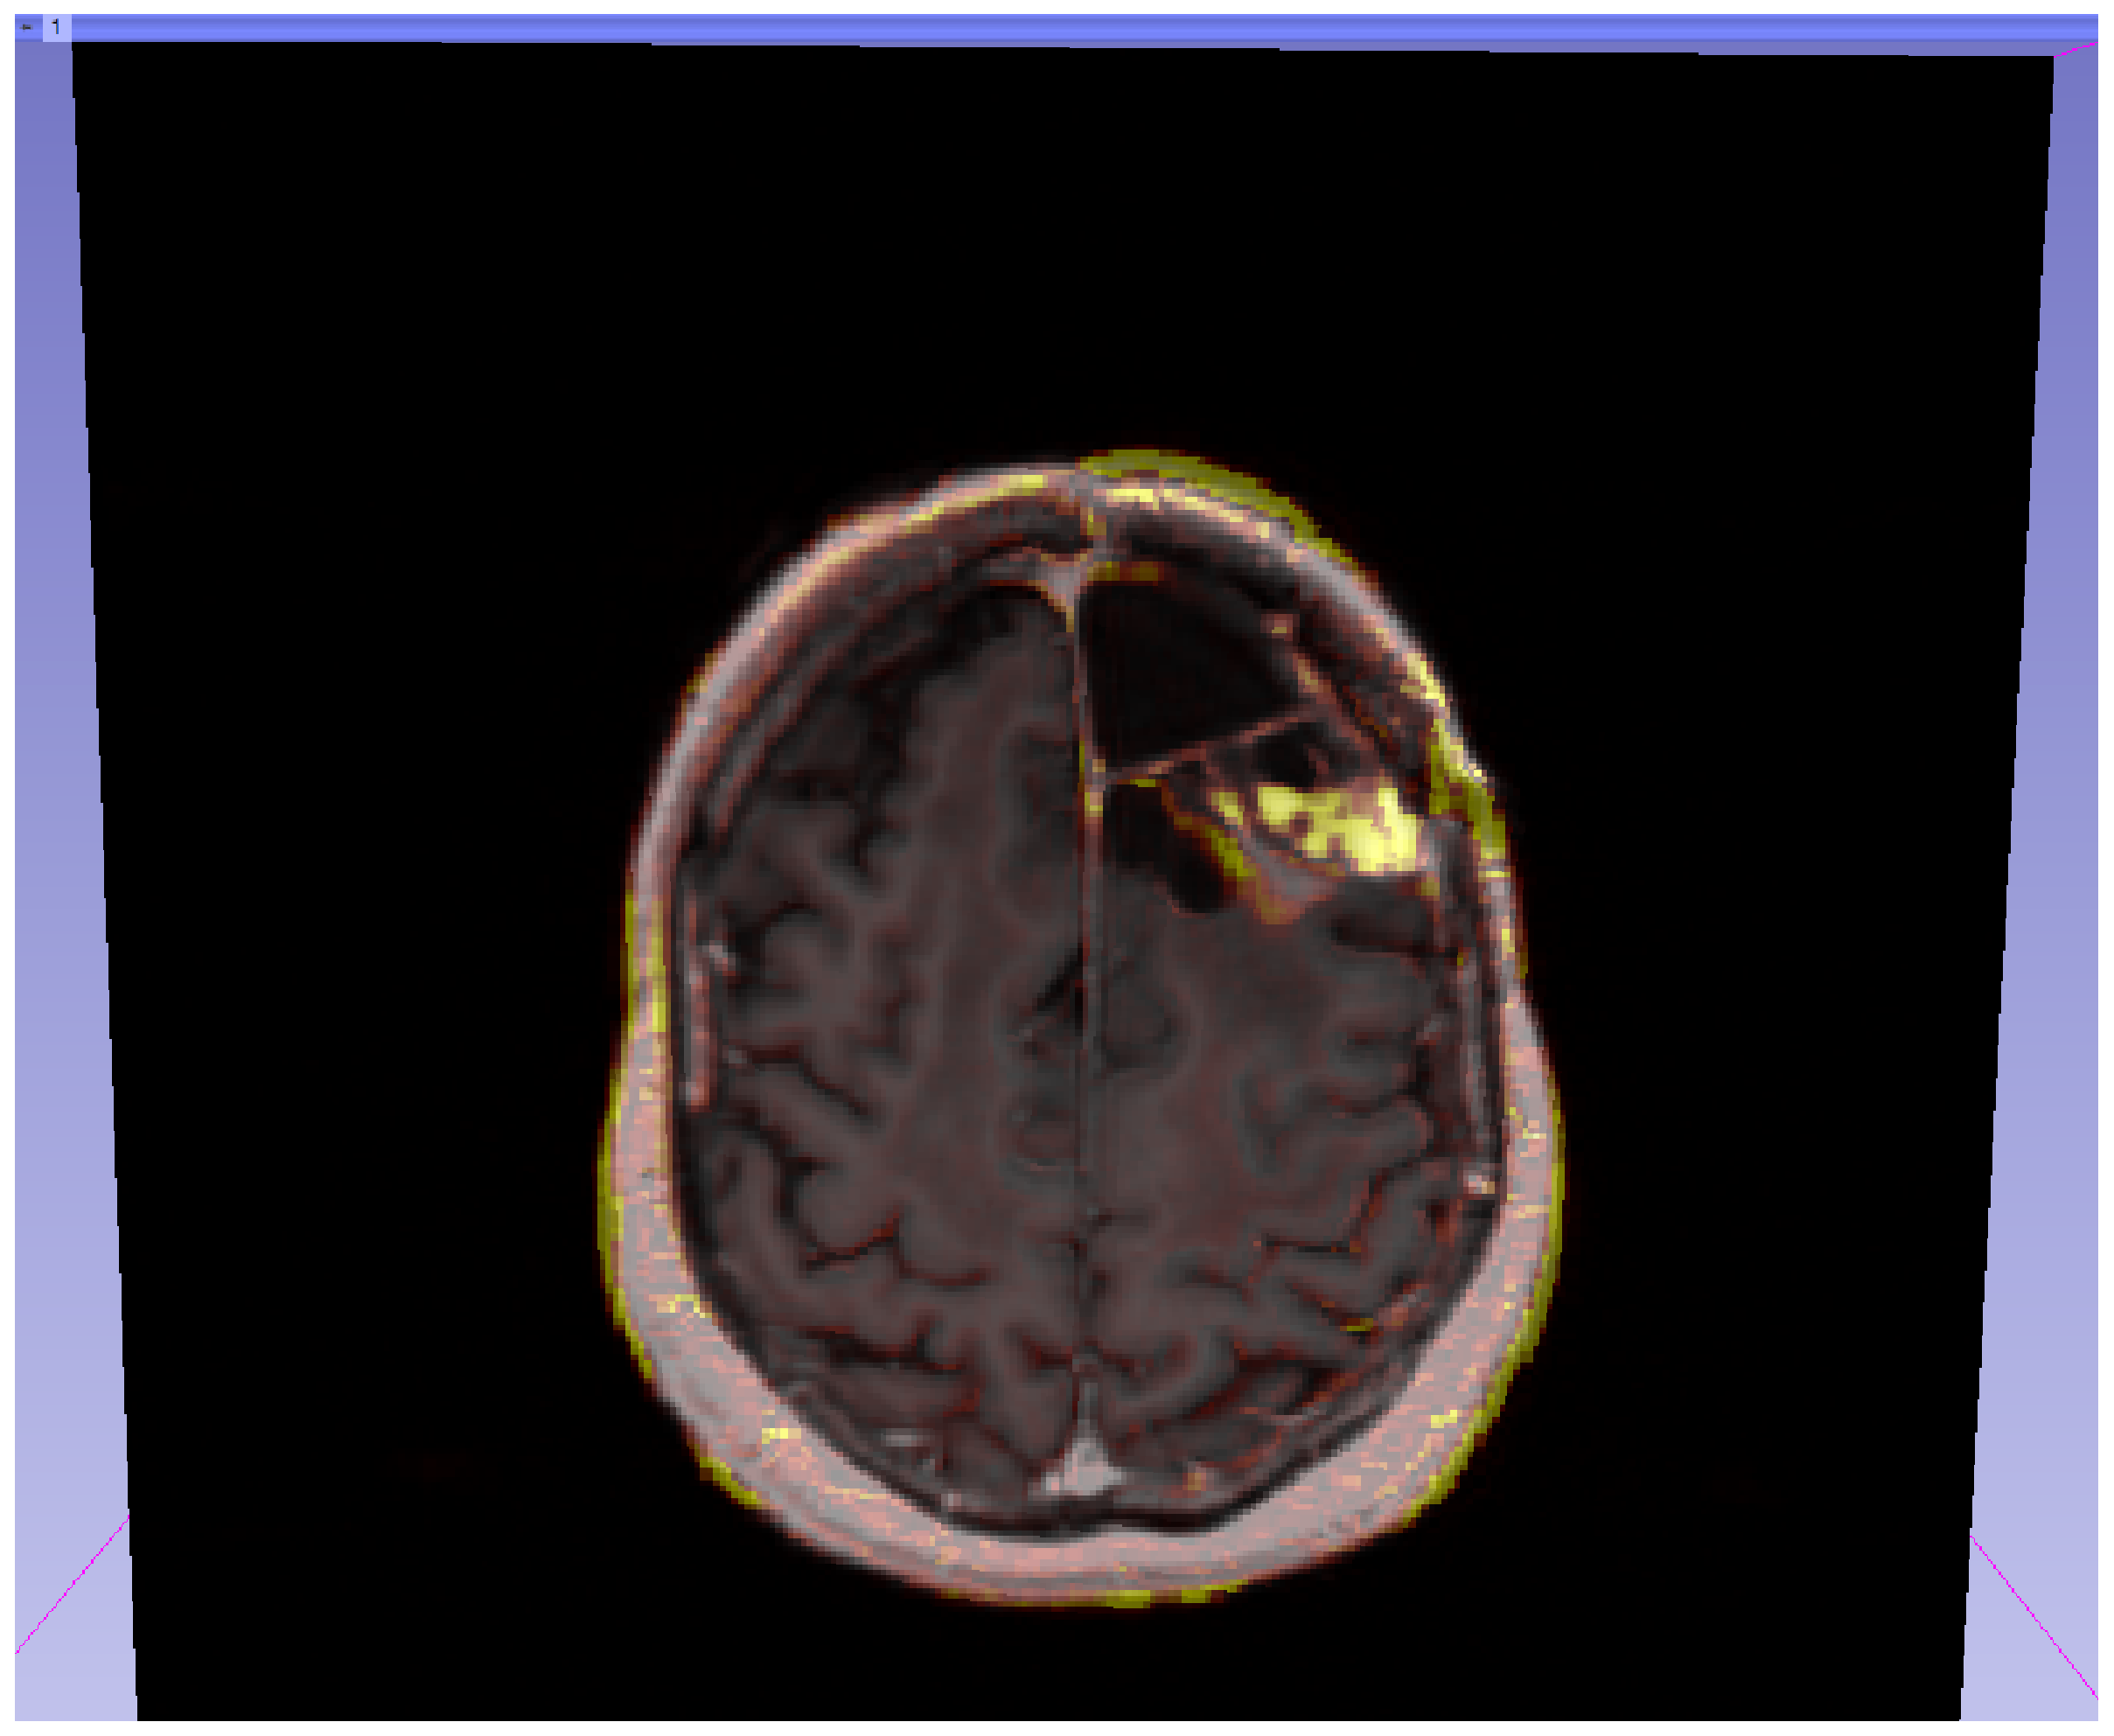
\includegraphics[scale=0.2]{/experiment_B2_P3/B2_Traversal2.eps}
  \caption{Voxel-based method. Patient 3: Upper traversal plane}
  \label{B2_Traversal2}
\end{figure}

\begin{figure}[H]
  \centering
  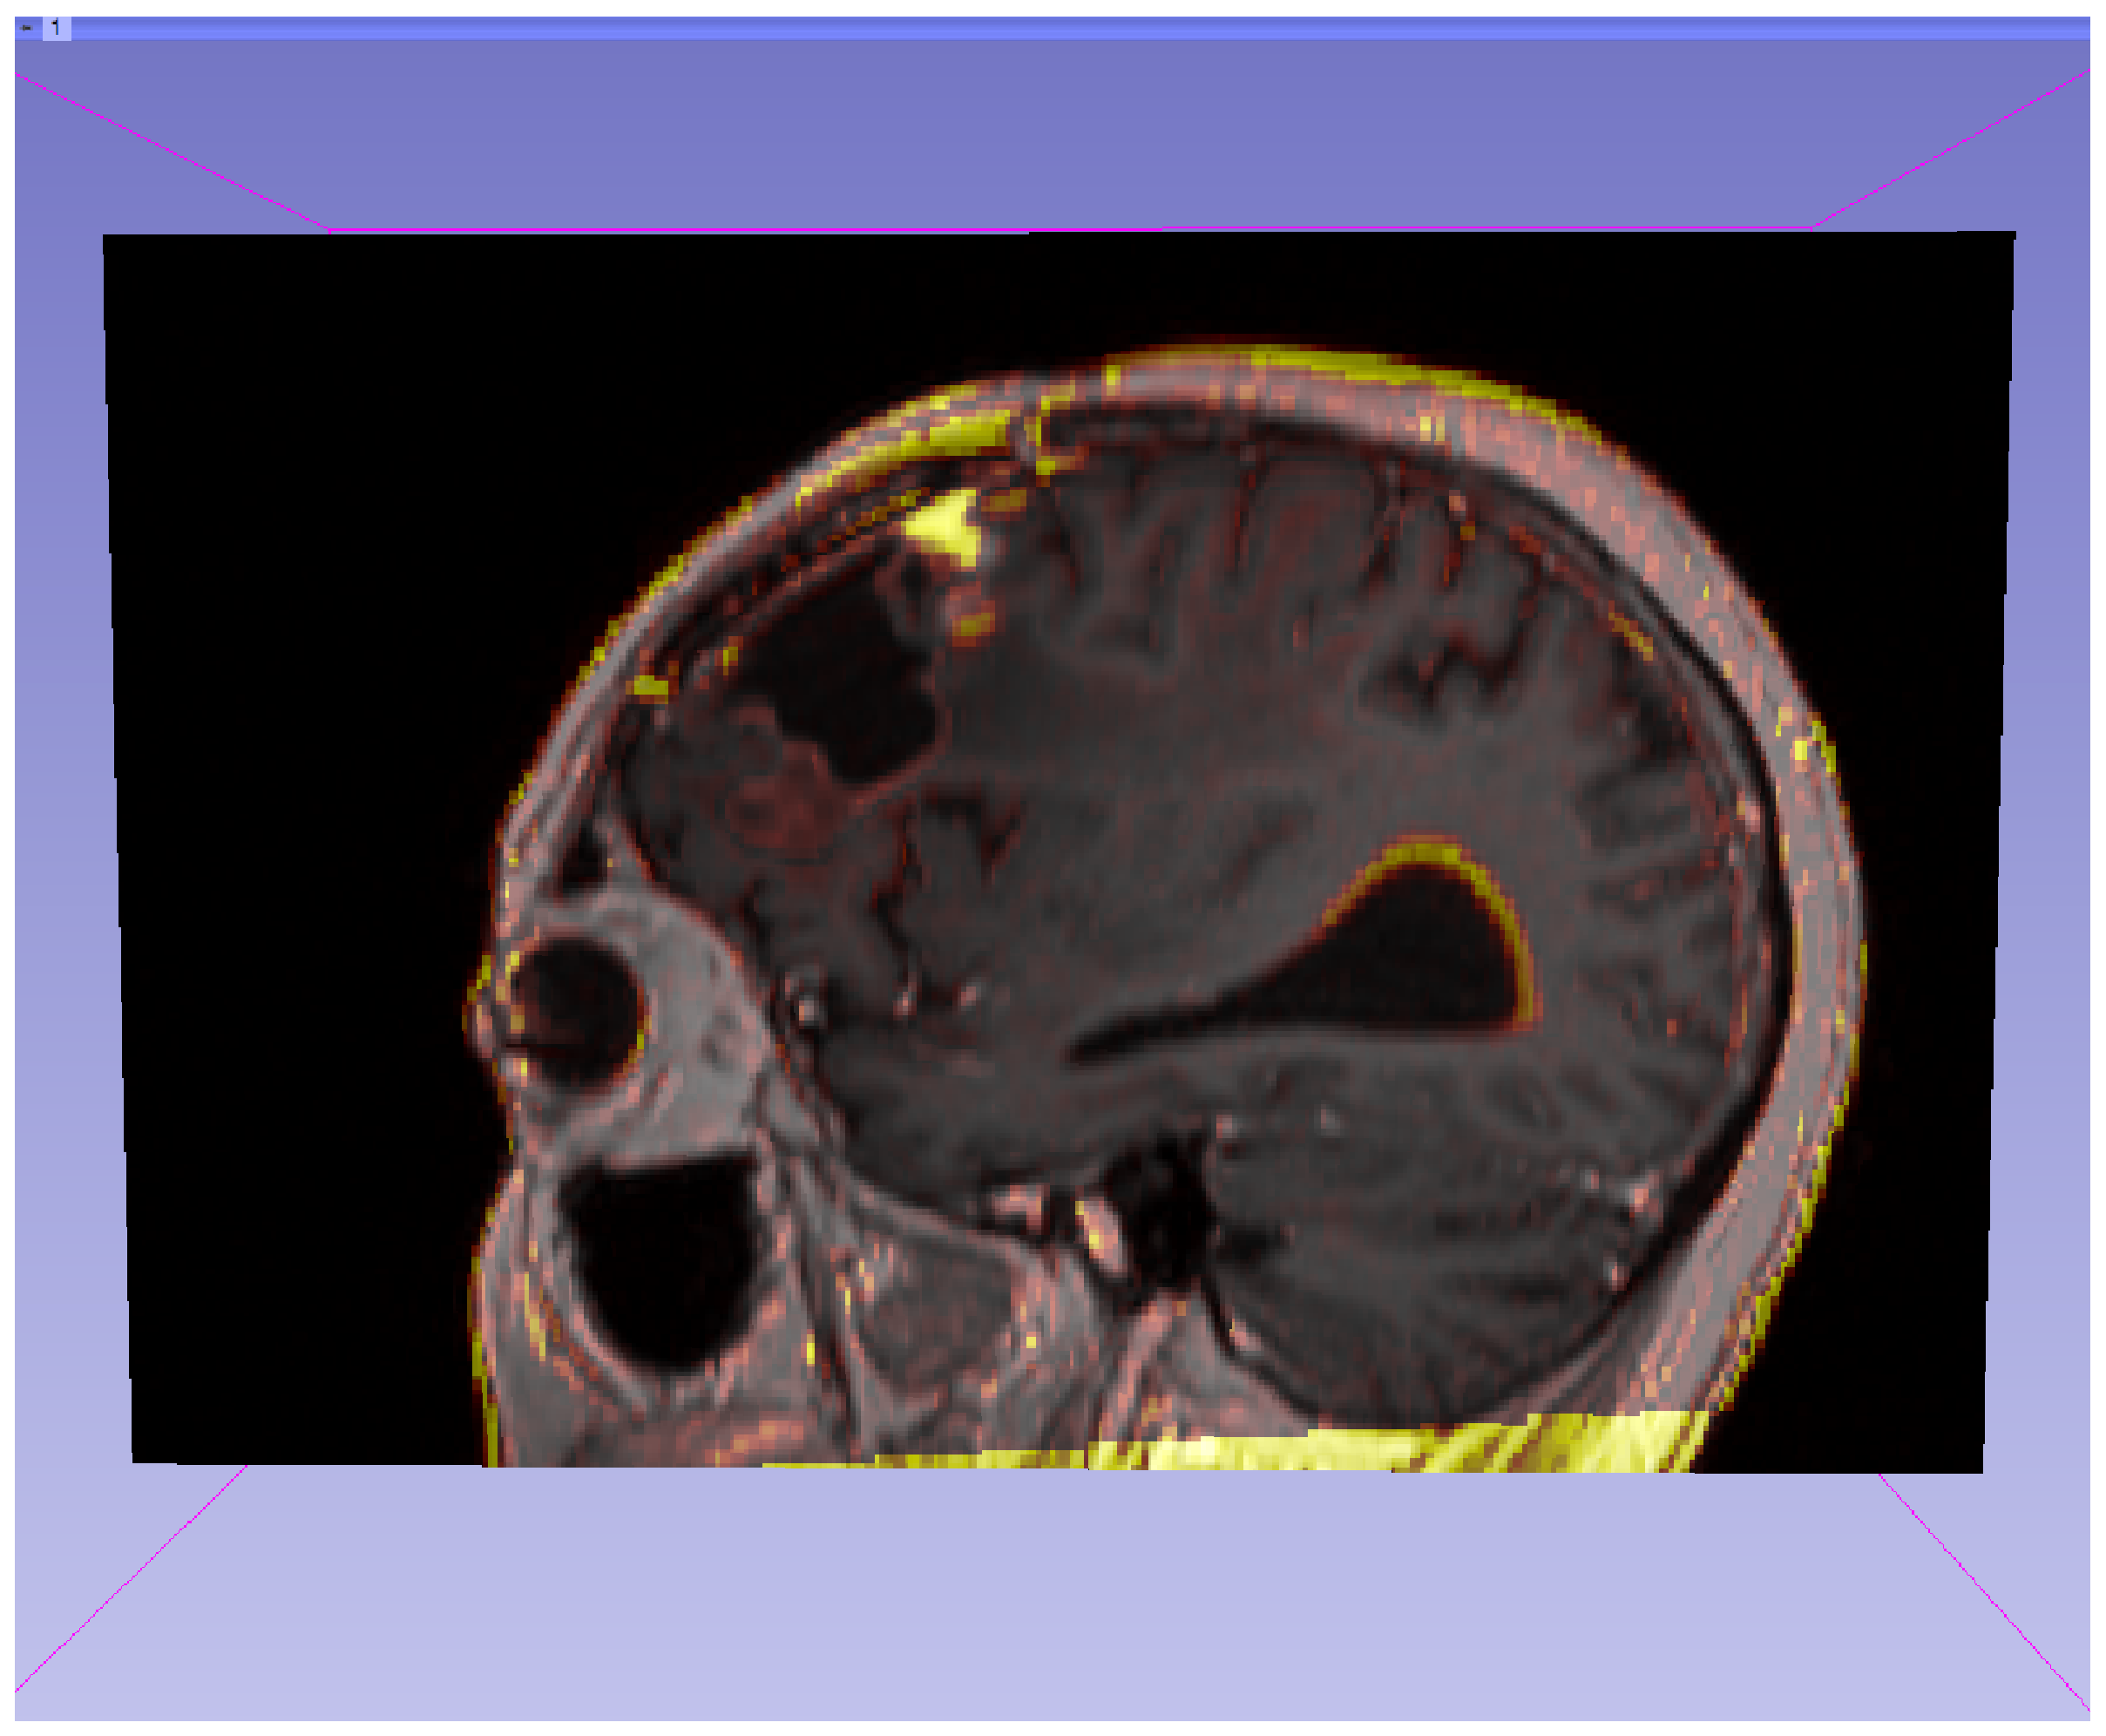
\includegraphics[scale=0.2]{/experiment_B2_P3/B2_Sagittal.eps}
  \caption{Voxel-based method. Patient 3: Sagittal plane}
  \label{B2_Sagittal}
\end{figure}


\subsubsection{Tensor-based Method}
This method also shows the expected difference due to the surgery
(correctly expressed as shrinkage, in green) which can be seen in the
images \ref{B2_TCoronal}, \ref{B2_TTraversal2} and \ref{B2_TSagittal}.

The image \ref{B2_TTraversal1} is showed for comparison with the
differences shown in image \ref{B2_Traversal1} in the previous
method. The tensor-based result doesn't show the exact same result;
however, some growth (in pink) can be seen. This could be attributed
to either inaccuracy of the method or to movement in the brain
consistent with the surgery.\\

Parameters used:
\begin{description}
\item \textit{Deformation field smoothing sigma:} 2.5
\item \textit{Shrinkage percentage:} 60
\item \textit{Growth percentage:} 50
\end{description}

\begin{figure}[H]
  \centering
  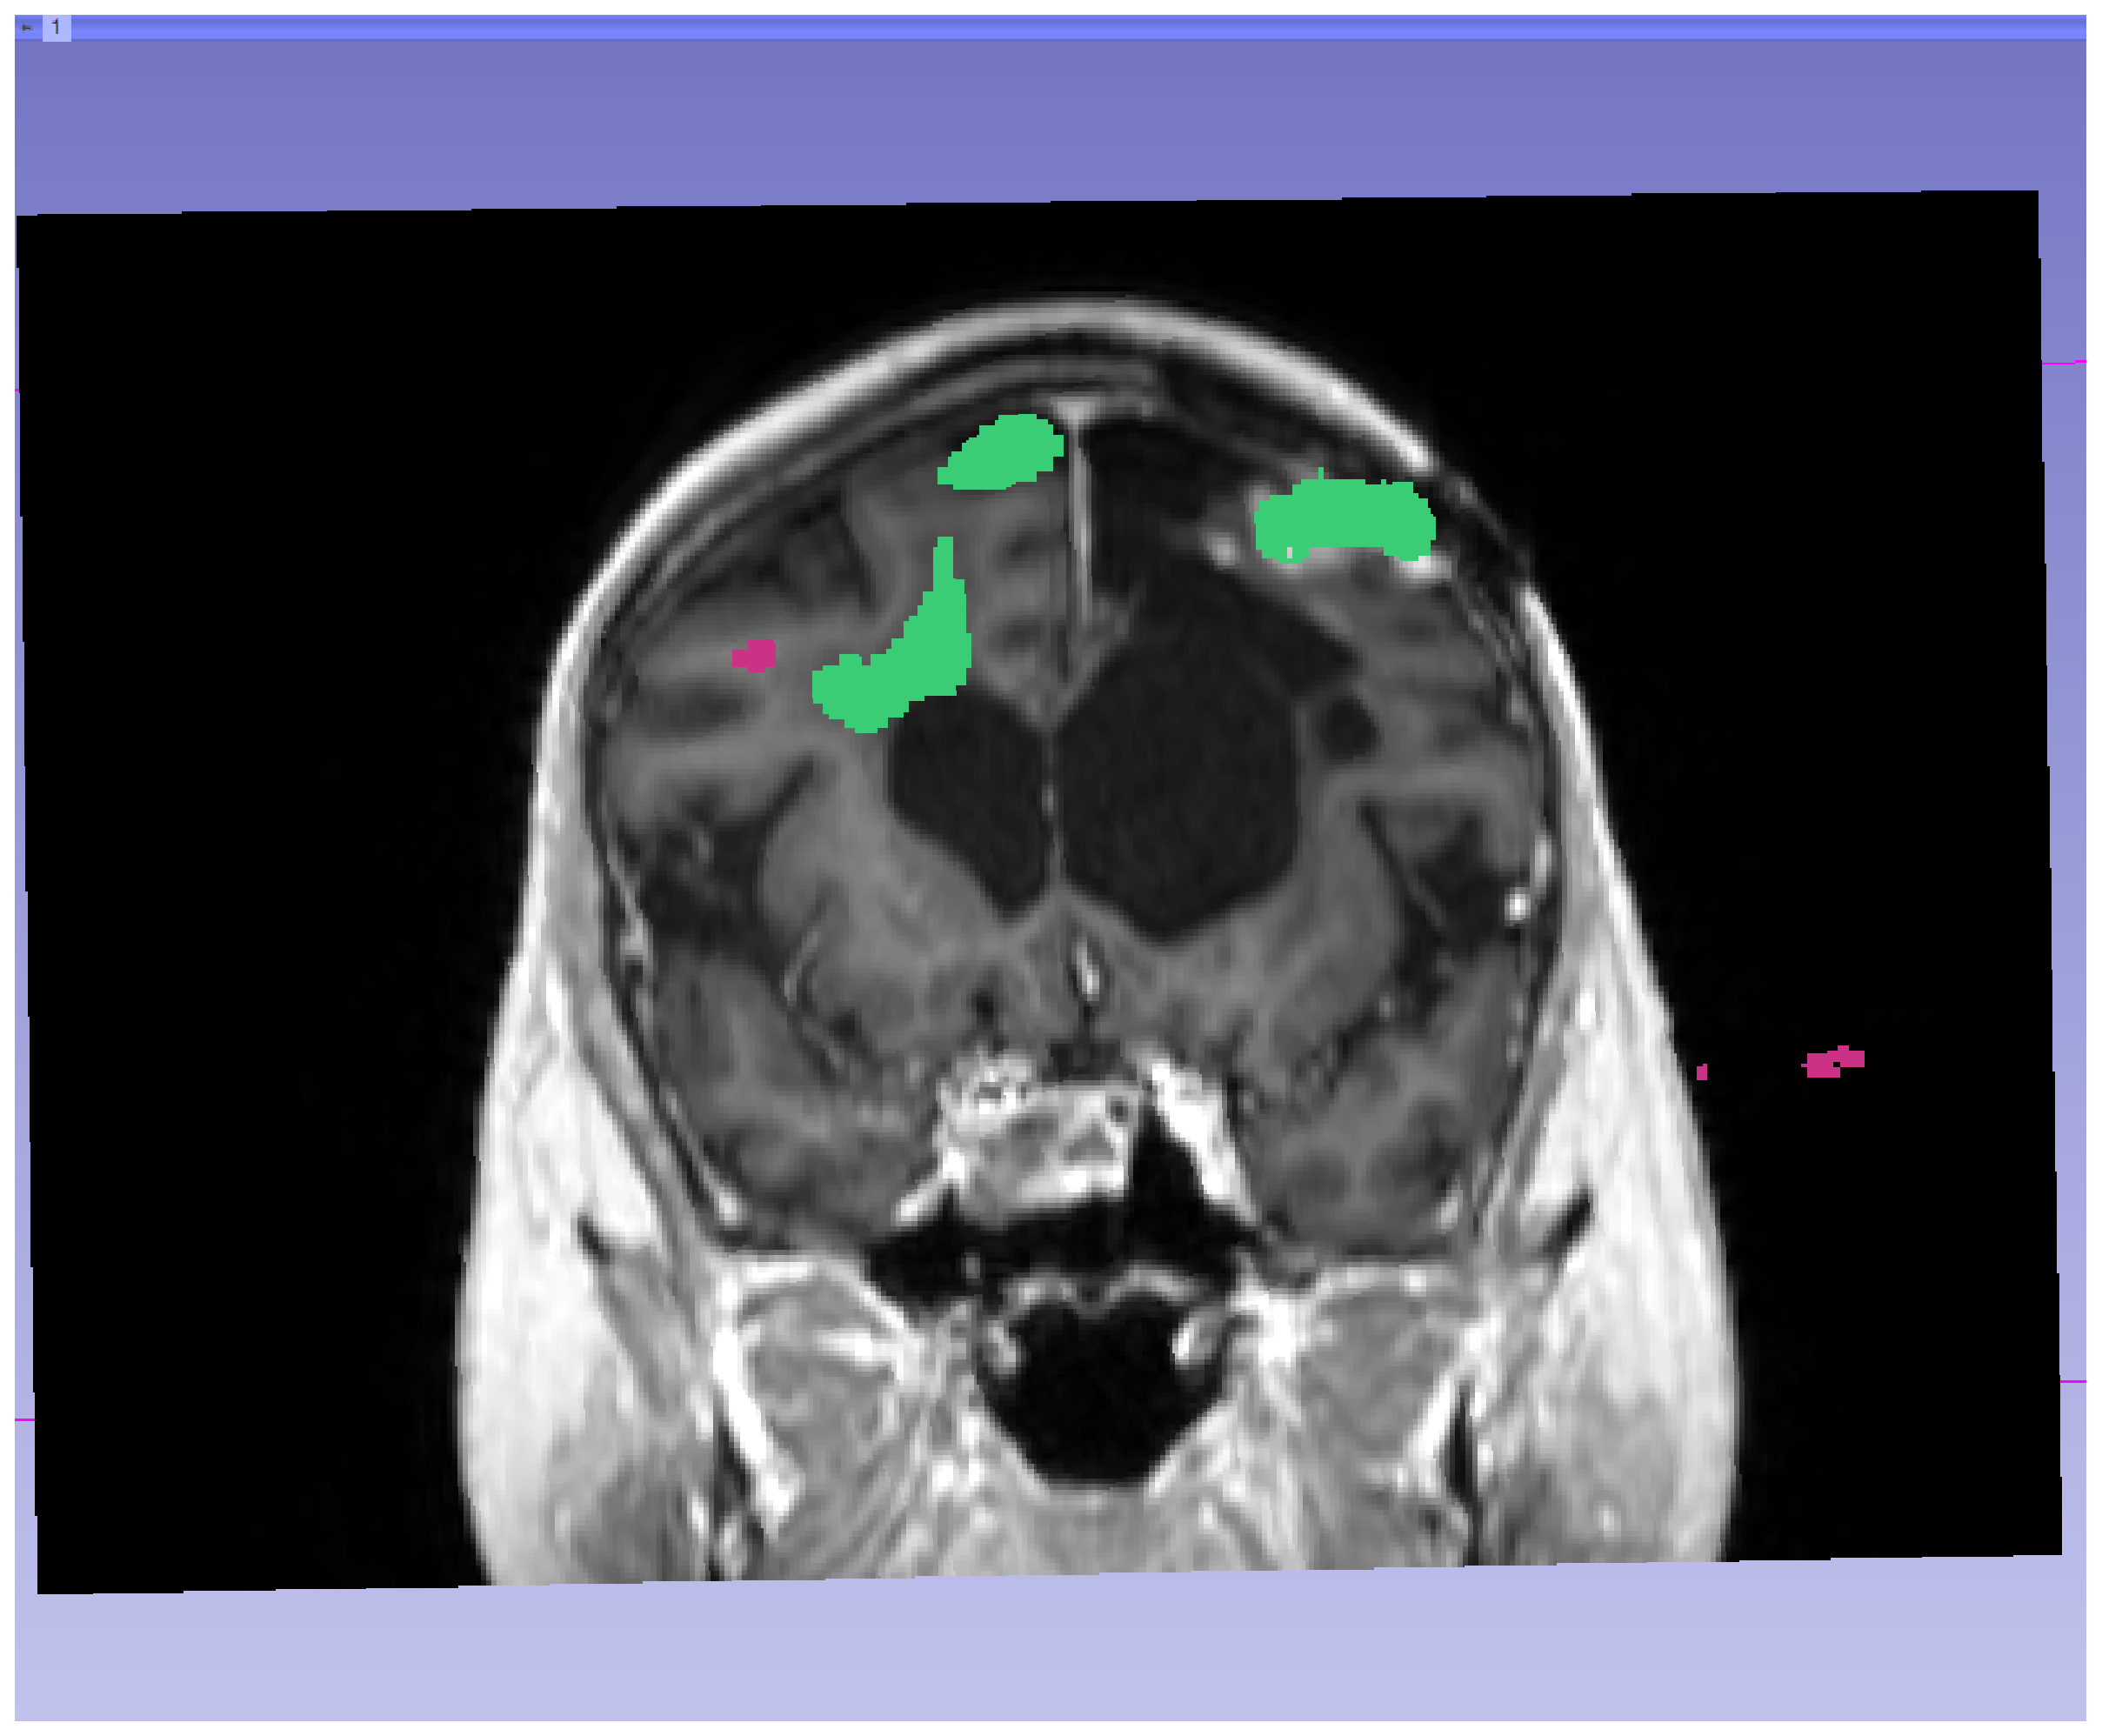
\includegraphics[scale=0.2]{/experiment_B2_P3/B2_Tensor_Coronal.eps}
  \caption{Tensor-based method. Patient 3: Coronal plane}
  \label{B2_TCoronal}
\end{figure}

\begin{figure}[H]
  \centering
  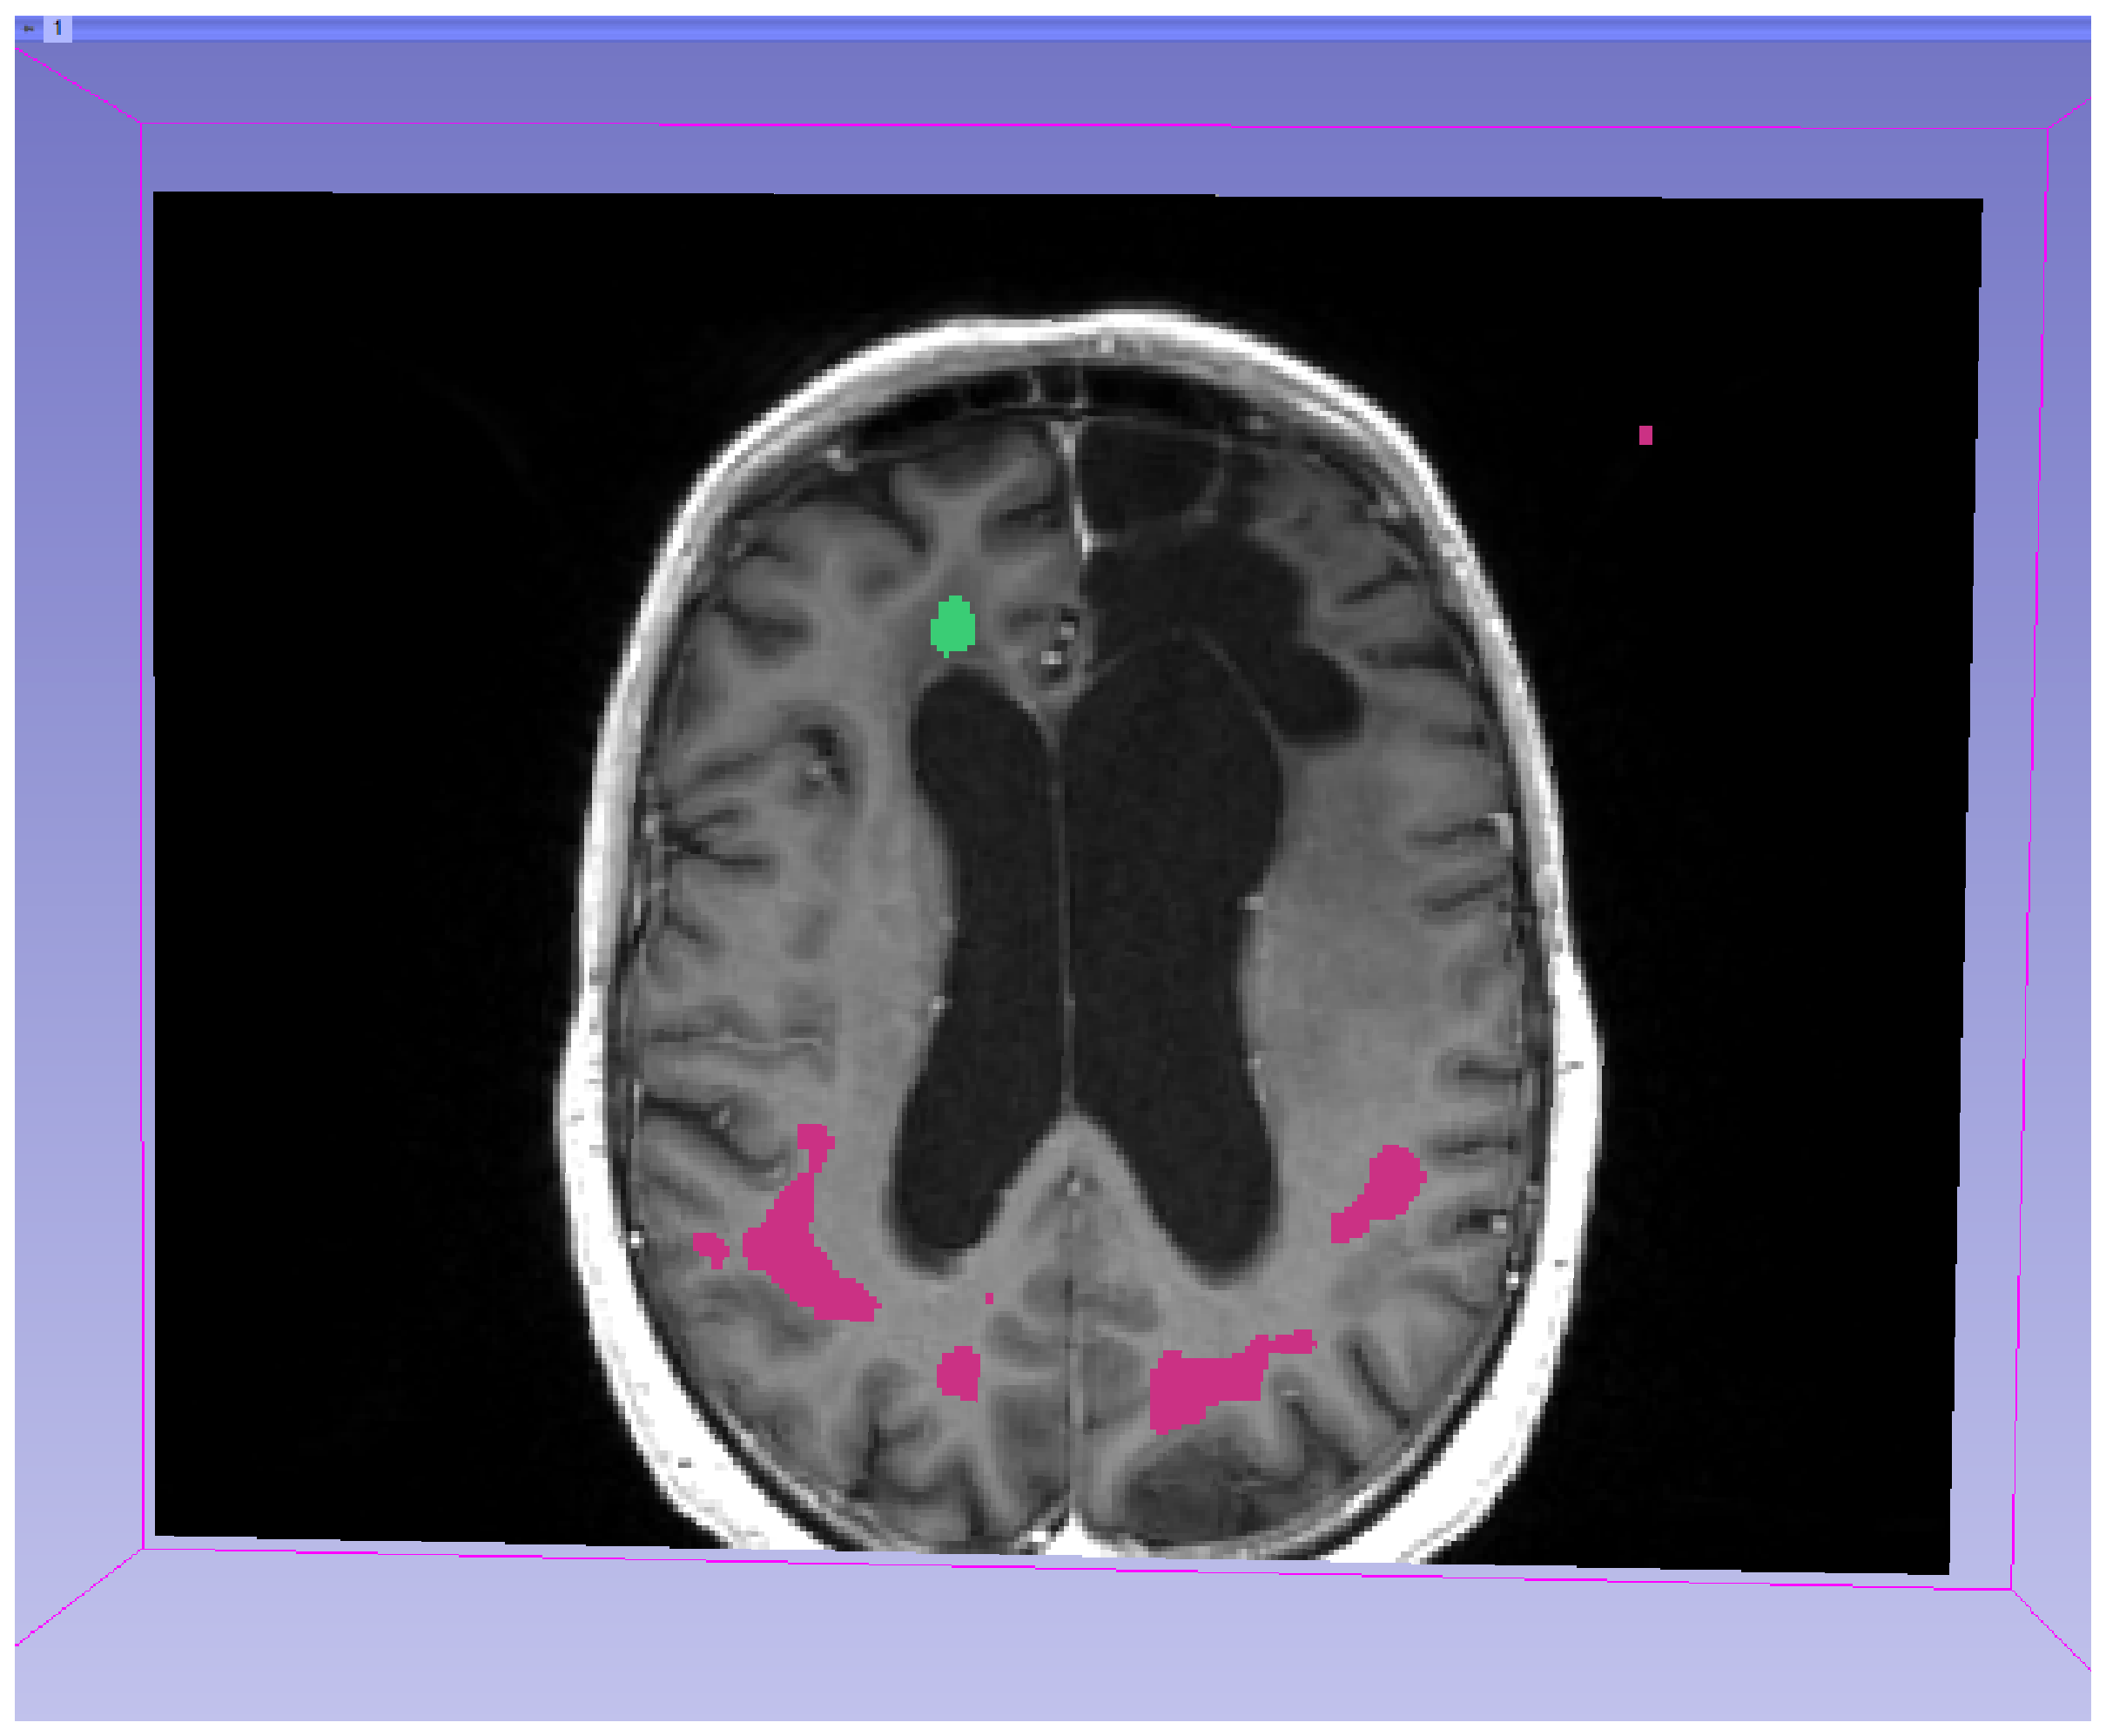
\includegraphics[scale=0.2]{/experiment_B2_P3/B2_Tensor_Traversal1.eps}
  \caption{Tensor-based method. Patient 3: Traversal plane}
  \label{B2_TTraversal1}
\end{figure}

\begin{figure}[H]
  \centering
  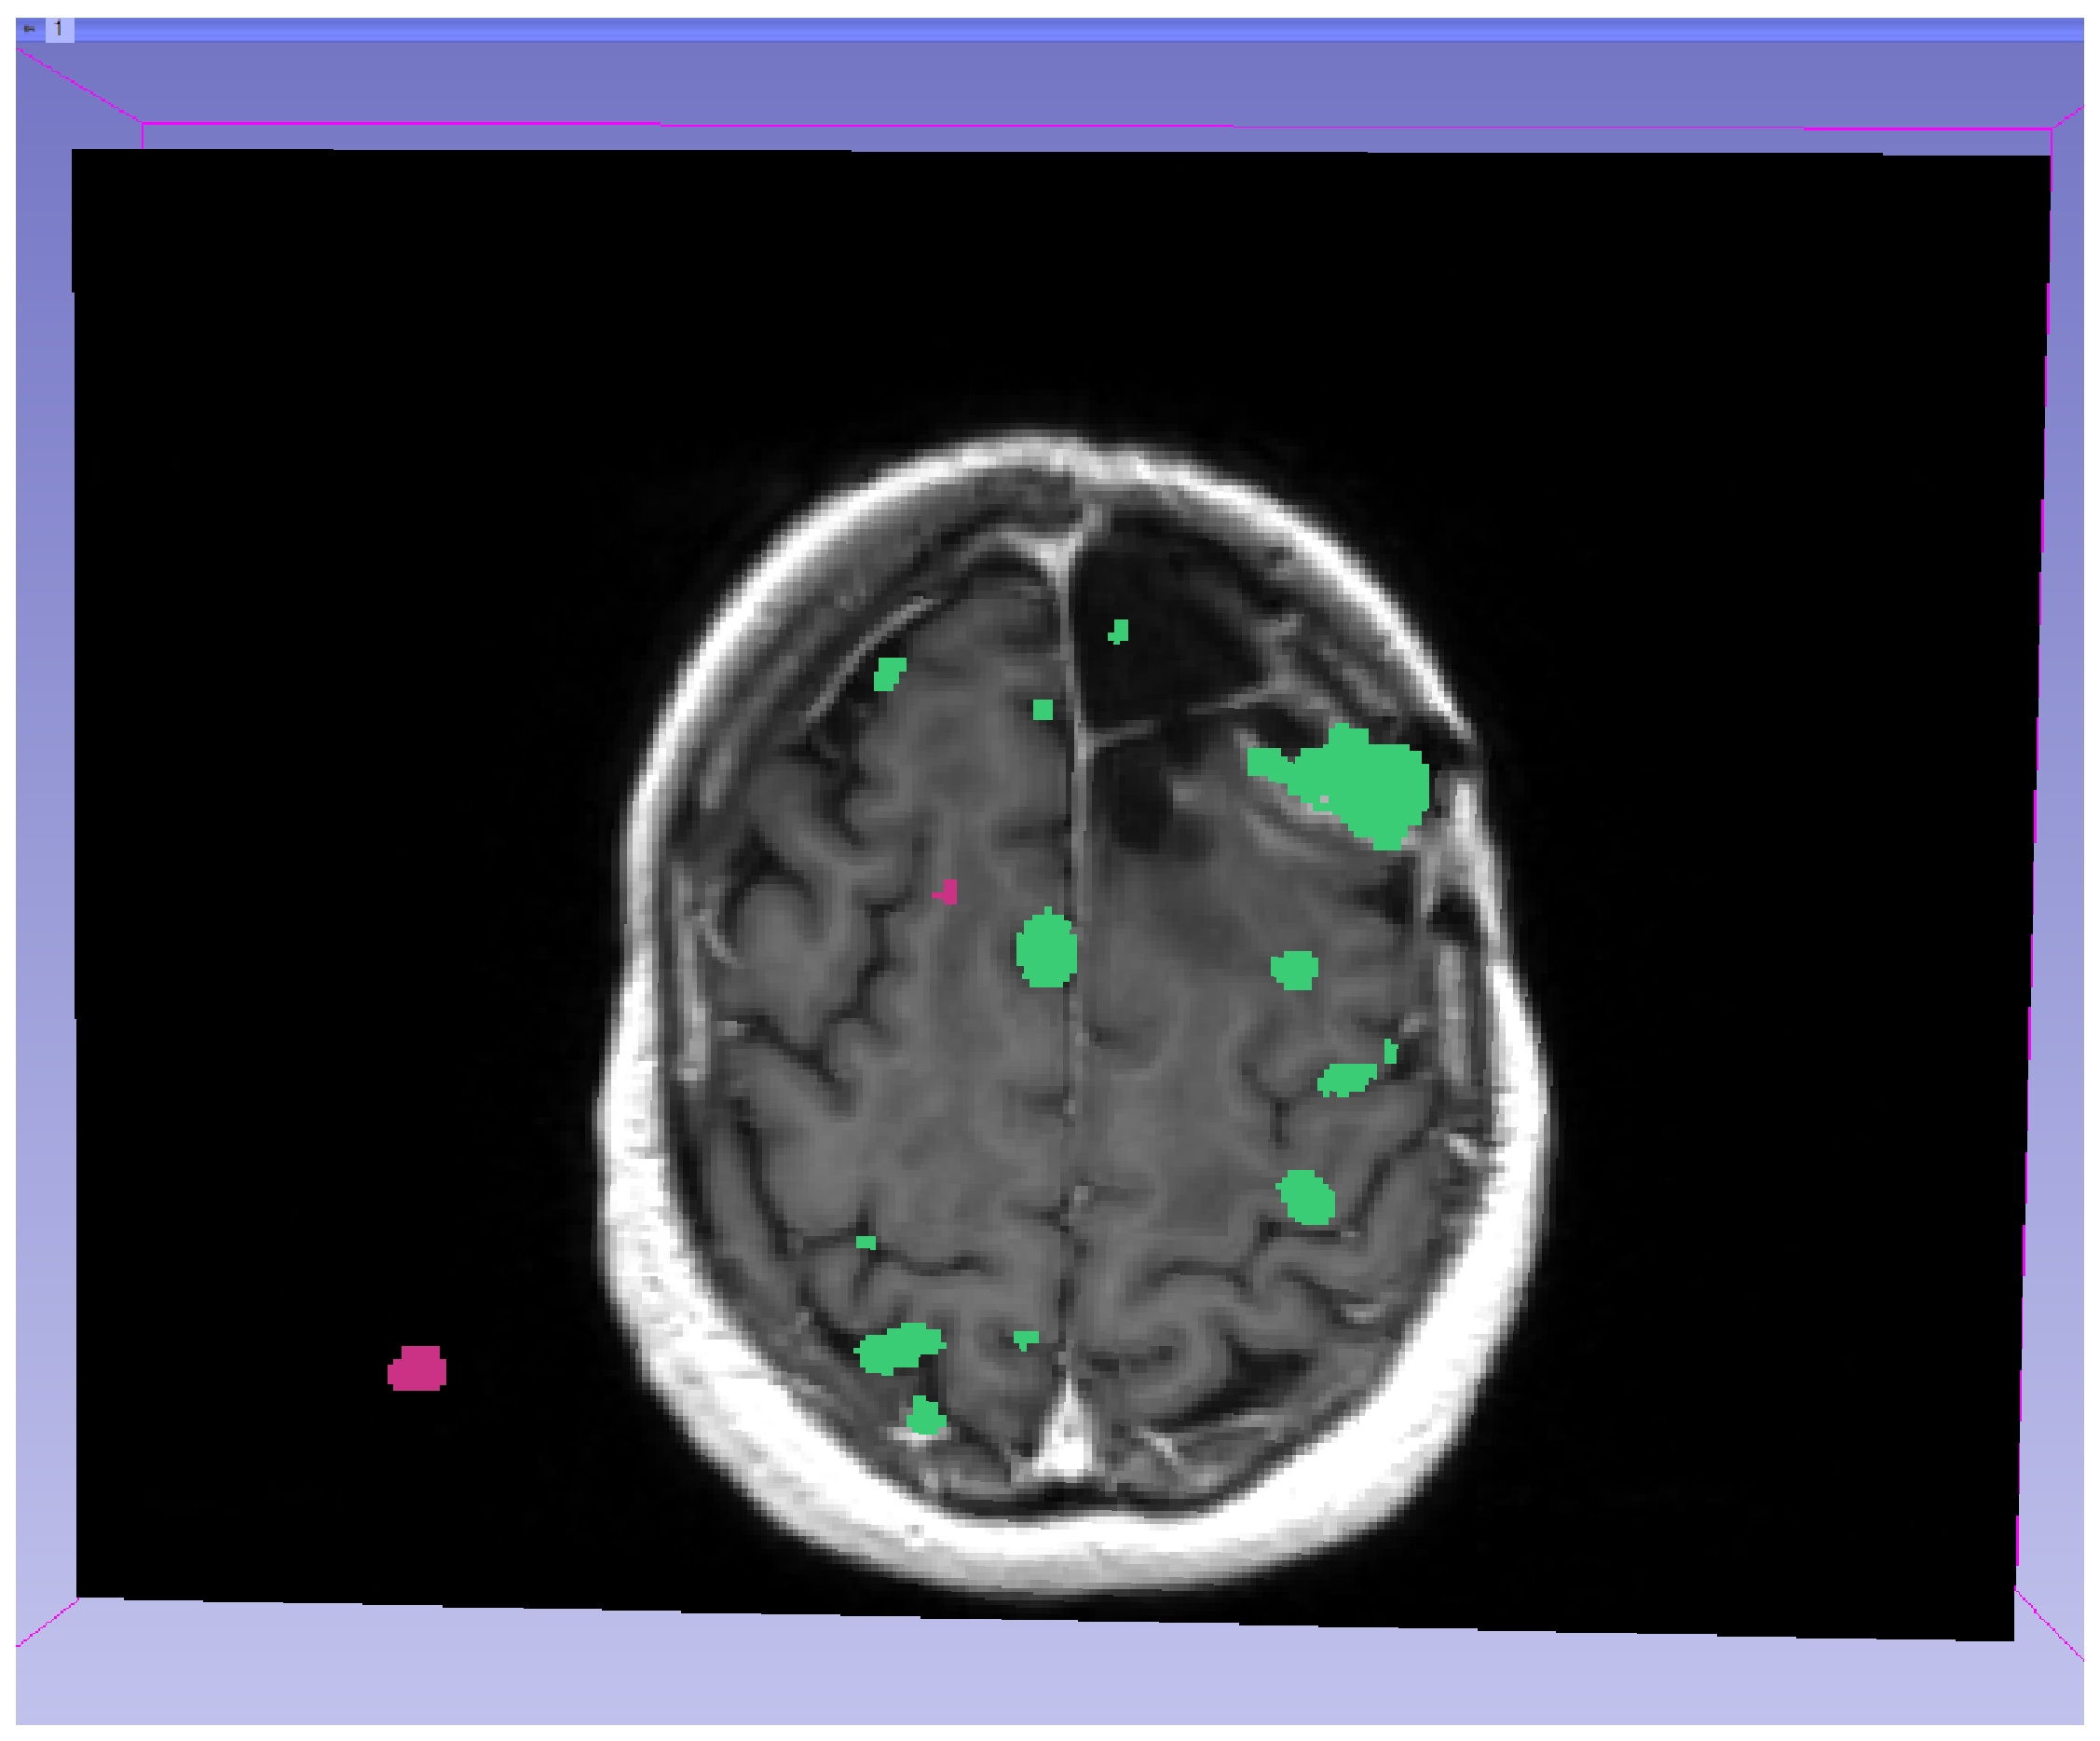
\includegraphics[scale=0.2]{/experiment_B2_P3/B2_Tensor_Traversal2.eps}
  \caption{Tensor-based method. Patient 3: Upper traversal plane}
  \label{B2_TTraversal2}
\end{figure}

\begin{figure}[H]
  \centering
  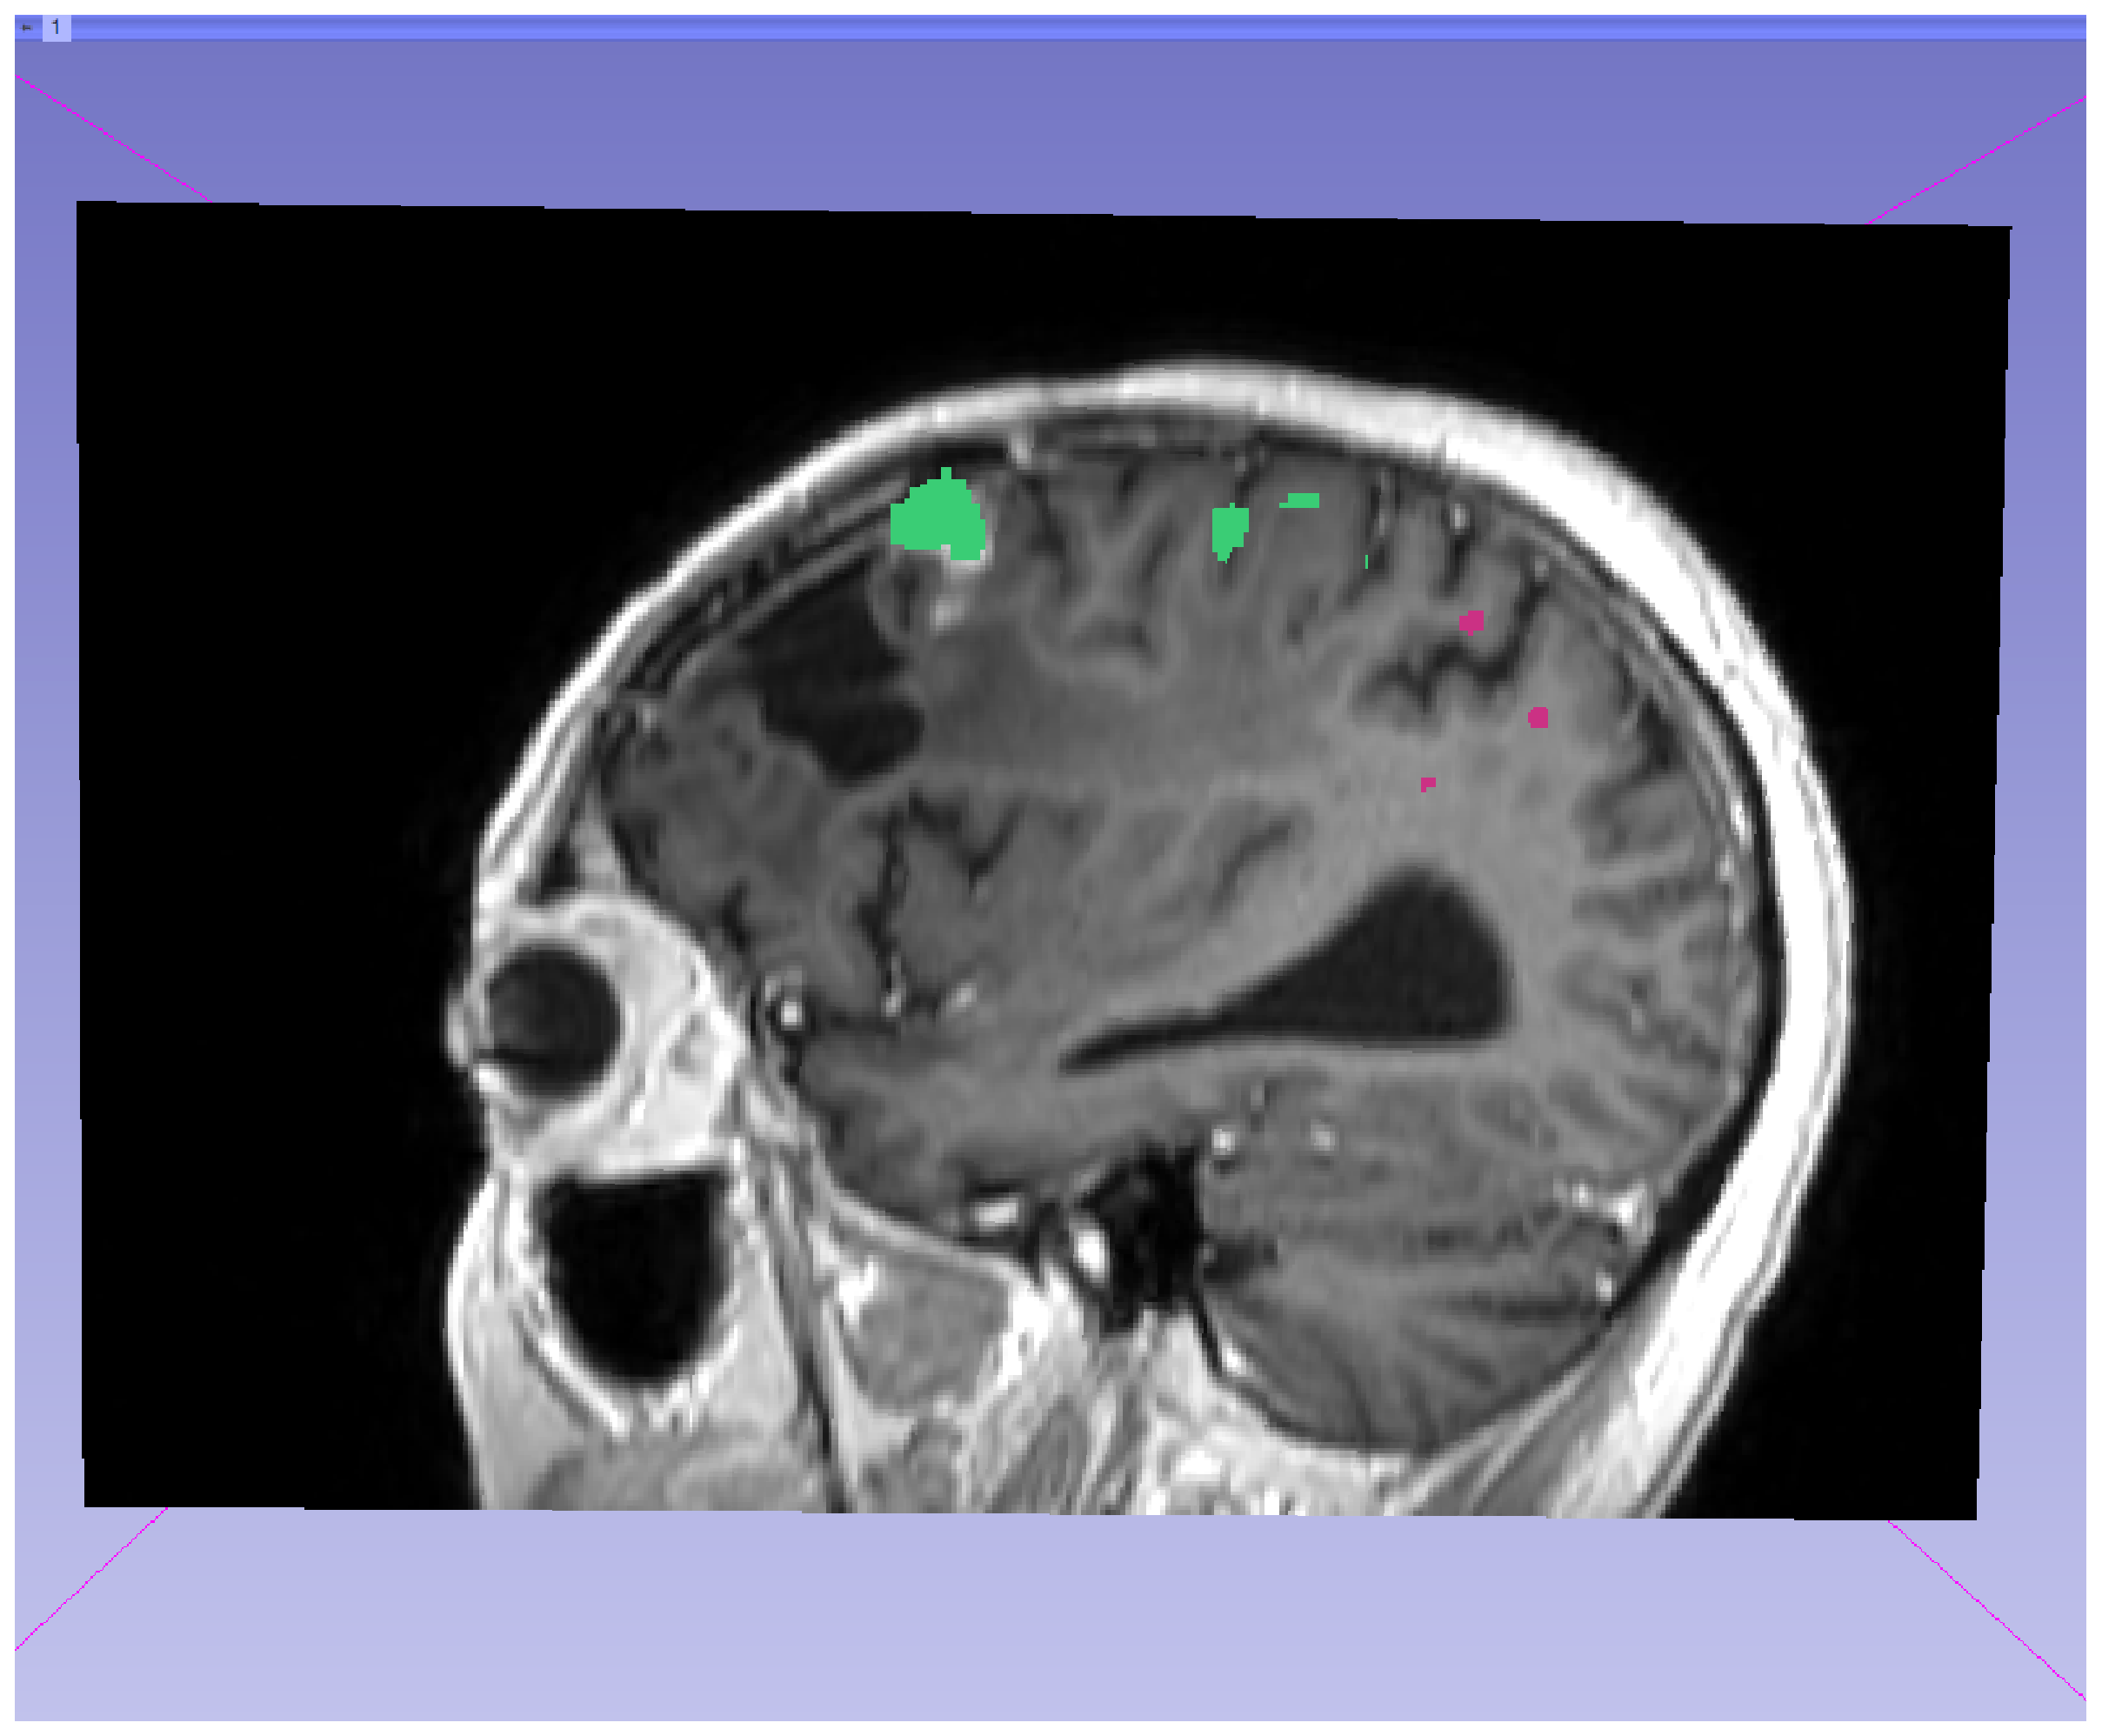
\includegraphics[scale=0.2]{/experiment_B2_P3/B2_Tensor_Sagittal.eps}
  \caption{Tensor-based method. Patient 3: Sagittal plane}
  \label{B2_TSagittal}
\end{figure}
     \chapter{Applications}

\section{Raili's study}

\section{other projects}
     \chapter{Conclusions}

The goal of detecting and locating small differences between images
and volumes presents a very interesting problem, not only limited to
the medical field. It is still a big challenge today for which a
complete solution is required.\\

Even though in our specific case we deal with patients that have
received mild trauma, it can still mean a lot for the quality of life
of a person if he or she receives help when needed, and if the
physician is able to locate the exact area affected by the injury.\\

The applications presented in this project were created as modules of
a bigger and already existent application called \textit{3D Slicer},
which contains many other functionalities for medical image analysis
and manipulation.

In this way, the applications are not only given an interface that is
easy to use, but also allow the user to utilize any of the
other modules already present within \textit{3D Slicer}.\\

The applications attempt to solve the problem for MRI volumes with two
different techniques, both obtained from analysis of previous research
done in the area.

The results obtained with the voxel-based method are quite good, even
when the artificial differences added where too small to be found with
the naked eye. During this research, this method was successfully used
in a medical study with real patients performed by the Uppsala
University Hospital.

The tensor-based method also produced useful results for differences
of large and medium size. Even though the results were not as expected
for smaller differences, the method could be the start for a very
interesting future development possibly using the \textit{Jacobian
  matrix}.\\

Finally, it is important to highlight that the results of both methods
as they are now, are just a suggestion of the size and location of the
differences between the volumes; as a consequence, the procedure can
not be completely automatic, since the applications still need the
help of a medical practitioner in order to define the differences more
exactly and possibly rule out errors.


\section{Future works}

The tensor-based method needs to be improved in order to obtain more
exact results, and for it to be able to detect smaller differences.

The first thing that should be done is either find a better way of
figuring out which range of values of the \textit{Jacobian
  determinant} are actually useful to detect differences, or directly
using the \textit{Jacobian matrix} to calculate the changes in volume
between the MRIs.

Manipulating the \textit{Jacobian matrix} is harder than using the
\textit{Jacobian determinant} since, according to my research, there
is no \textit{ITK} function or library already implemented to use
it. Some theoretical pointers on how to use the matrix can be found in
\cite{ashburner}.\\

The voxel-based method seems to work quite well in our experiments
with both real and artificial differences between volumes. However, it
would be very interesting to be able to compare its results against
another tool with the same goals.\\

We would like the modules to be available for all the users of
\textit{3D Slicer} and for the public in general. To achieve this
goal, a few specific conditions must be fulfilled in order for the
module to be accepted as part of the \textit{3D Slicer} code.

This would probably produce some criticism from the \textit{3D Slicer}
developer community, which could contain useful comments on the
current implementation of the modules and how to improve it.\\





\backmatter
    \nocite{*} % Remove this for your own citations
    \bibliographystyle{plain}
    \bibliography{References}

\end{document}